\documentclass[newpage,numbers,handout]{ximera}
%% handout
%% nohints
%% newpage

\usepackage{microtype}
\usepackage{tikz}
\usepackage{tkz-euclide}
\usetkzobj{all}
\tikzstyle geometryDiagrams=[ultra thick,color=blue!50!black]

\renewcommand{\epsilon}{\varepsilon}



\let\masterdocument\document
\let\endmasterdocument\enddocument

\begin{masterdocument}
\begin{titlepage}
    \vspace*{1in}
    \begin{center}
      {\Huge \bfseries Workbook of two-dimensional geometries}\\[0.5cm]
      {\Large C.\ Herbert Clemens}\\[0.4cm]
      This document was typeset on \today.
    \end{center}
    %\vspace*{\fill}
  \end{titlepage}

\tableofcontents

\renewcommand{\documentclass}{\setbox0\vbox}
\renewcommand{\preambleinput}{\setbox0\vbox}
\renewenvironment{document}{}{}

\documentclass{ximera}
\usepackage{microtype}
\usepackage{tikz}
\usepackage{tkz-euclide}
\usetkzobj{all}
\tikzstyle geometryDiagrams=[ultra thick,color=blue!50!black]

\renewcommand{\epsilon}{\varepsilon}



\title{Introduction}

\begin{document}
\begin{abstract}
Seeing different geometries as a variation on a theme.
\end{abstract}
\maketitle

As a young mathematician I was introduced to the classic \textit{Le\c{c}ons
sur la G\'{e}om\'{e}trie des Espaces de Riemann}, written by the great French
geometer \'{E}lie Cartan. Early in his treatise on geometries in all
dimensions, the author presents the case of two-dimensional geometries, in
particular, those two-dimensional geometries that look the same at all points
and in all directions. (For example, a cylinder looks the same at each of its
points but not in all directions emanating from any one of its points, whereas
a sphere looks the same at all points and in all directions.) It turns out
that there is one and only one such geometry for each real number $K$, called
the \textit{curvature} of the geometry. The case $K=0$ is the (flat) Euclidean
geometry that you learned in high school.

These twenty-five pages of Cartan's book (Chapter VI, \S i-v) so captivated me
that I have returned to them regularly throughout my career and have adapted
and taught them many times at the advanced undergraduate level. They form the
basis for this little book. To me they tell one of the most beautiful and
satisying stories in all of geometry, one which exemplifies a fundamental
principle of all great mathematics, namely that, using the tools at hand but
in a slightly novel way, the clouds part and one sees that objects and
relationships that seemed so different are in fact parts of a single elegant story!

When $K>0$ it turns out that the $K$-geometry is the geometry of the sphere of
radius $R=1/K^{1/2}$ that we can see as a subset of Euclidean three-space
$\mathbb{R}^{3}$. But the geometries with $K<$ $0$ are not so easy to
visualize. They are the so-called `hyperbolic' geometries. In fact it took
mathematicians a couple thousand years to realize that the existed at all! It
turns out that the secret to understanding all the two-dimensional geometries,
including the ones with $K<0$, in a unified way is to simply rescale the third
coordinate in $\mathbb{R}^{3}$ and, in these `unusual' coordinates $\left(
x,y,z\right)  $, to look at each two-dimensional geometry as the solution set
to the equation%
\[
K\left(  x^{2}+y^{2}\right)  +z^{2}=1.
\]
However the idea of changing coordinates without changing the underlying
geometry described by those coordinates is a challenging one that did not come
into mathematics until a couple of centuries ago. It will require that, before
we get into the beautiful uniform study of all two-dimensional geometries, we
practice the coordinate change we are going to use, namely the rescaling of
the third coordinate in Euclidean $3$-space. That practice, together with a
review of some concepts from several variable calculus and linear algebra,
will comprise much of this book.

It has often been said that ``mathematics is not a spectator sport.''
This truism is very much in evidence in the writing of this book. It
is written so as to guide you through the entire story, yet permit
you, when possible, to construct the mathematical story for yourself,
that is, to do some mathematics yourself rather than just observe it
done by others. This `doing mathematics oneself' takes the form of
Exercises with enough help (Hints) provided so that the `doing' is not
so onerous as to get in the way of the story itself.

Strong evidence has been provided by students of mathematics over many
centuries that such guided `doing' is indispensible for understanding and
retention. In fact the very form of this book, as a loose-leaf or electronic
notebook, is intended to encourage you to write out (in correctable form)
solutions to the problems that can be inserted at the appropriate places into
the text.

This book supposes familiarity with several variable calculus and the linear
algebra of matrices. In particular you will need to remember and apply the
chain rule for differentiable functions of several variables, written in
matrix notation. That is:

\begin{theorem}
\textbf{(Chain Rule)} Given differentiable mappings%
\begin{align*}
&  \left(  y_{1}\left(  x_{1},\ldots,x_{m}\right)  ,\ldots,y_{n}\left(
x_{1},\ldots,x_{m}\right)  \right) \\
&  \left(  z_{1}\left(  y_{1},\ldots,y_{n}\right)  ,\ldots,z_{p}\left(
y_{1},\ldots,y_{n}\right)  \right)
\end{align*}
then%
\[
\left(  \frac{\partial z_{k}}{\partial x_{i}}\right)  =\left(  \frac{\partial
z_{k}}{\partial y_{j}}\right)  \cdot\left(  \frac{\partial y_{j}}{\partial
x_{i}}\right)  .
\]

\end{theorem}

As a help, at some points in the text and in some of the Exercises, a more
complete treatment of a particular topic can be found in one of the following
two texts:

[MJG]: Greenberg, Marvin Jay. \textit{Euclidean and Non-Euclidean Geometry:
Development and History.} W.H. Freeman \& Co. 3rd Ed., 1994.

[DS]: Davis, H. and Snider, A.D. \textit{Introduction to Vector Analysis.} Wm.
C. Brown Publishers, 7th Ed. 1994.

The corresponding topics in these texts are referenced. For example, [MJG,311]
refers to page 311 in the Greenberg book and [DS,59ff] refers to page 59 and
those pages just following page 59 in the Davis-Snider book.

Some final remarks about notation in this book. The letters `\textbf{EG}' will
always mean Euclidean (usually plane but occasionally $3$-dimensional)
Geometry, the letters `\textbf{SG}' will always mean Spherical Geometry, and
the letters `\textbf{HG}' will always mean Hyperbolic Geometry. One further
kind of geometry, which we call Neutral Geometry, will be explained in the
book and denoted by `\textbf{NG}.'

Also, it will often be useful to consider a vector, for example
$V=\left(a,b,c\right)$, as a $1\times3$ matrix
\[
V=
\begin{bmatrix}
a & b & c
\end{bmatrix}
\]
with
\[
V^\transpose  =
\begin{bmatrix}
a\\
b\\
c
\end{bmatrix}.
\]
This will allow us to write the scalar product of two vectors%
\begin{align*}
V\bullet W  &  =\left(  a,b,c\right)  \bullet\left(d,e,f\right) \\
&  =ad+be+cf%
\end{align*}
as a product of matrices%
\[
V\cdot W^\transpose=
\begin{bmatrix}
a & b & c
\end{bmatrix} 
\cdot
\begin{bmatrix}
d\\
e\\
f
\end{bmatrix}.
\]


It is my hope and intention in writing this little book that you engage with
and enjoy this uniform way of understanding all two-dimensional geometries as
much as I did!

\begin{remark}
Special message to current or future teachers of high school geometry:
Many parts of this book are especially relevant to your teaching of
the subject. Look especially closely at the treatment of congruence
(rigid motion), similarity (dilation), circles, expressing geometric
properties with equations, and geometric measurement and dimension,
and compare them with the high school geometry sections of the Common
Core State Standards in Mathematics. The latter can be found at:
\end{remark}

\begin{center}
http://www.corestandards.org/Math/Content/HSG/introduction.
\end{center}

A useful companion course to one based on this book, one that might be
called \textit{Geometry for Teaching}, would explicitly make the
connections between the material covered as in this book and what you
do (or will do) in your high school geometry classroom. The idea is
\textit{not} that the material we will cover will tell you how to
teach that material but rather that the treatment given here will give
you the depth and breadth of geometric understanding that will allow
you to design what you teach and bring it into your classroom in ways
that those who lack that understanding cannot.

\begin{remark}
This book can also be used as a bridge to a first course in Riemannian
geometry. It treats the case of two-dimensional geometries that are
homogeneous, that is, that look the same at all their points. But to treat
these geometries efficiently, we introduce the notion of changing coordinates
for the geometry without changing the geometry itself. It is that notion that
allowed geometers to treat surfaces and higher-dimensional smooth spaces that
look different at different points, ones that can often not be treated at all
their points using a single set of coordinates.
\end{remark}
\end{document}

\documentclass{ximera}

\preambleinput{../preamble.tex}

\prerequisites{rigidMotions,geometry}
\outcomes{neutralGeometry}

\title{Euclid's postulates for plane geometry} % the title of the activity
\begin{document}
\begin{abstract}
In this activity we explore neutral geometries.
\end{abstract}
\maketitle



\subsection*{Neutral geometry}

%% We first turn our attention to plane (or `flat') two-dimensional
%% geometry.

In Western civilization, the primary source of our understanding of
this geometry comes from Euclid's \textit{Elements}. The treatise is
of transcendant importance well beyond geometry itself, because it is
among the first, and perhaps the most influential single example of
organized, formal logical deductive reasoning. Certain fundamentals,
that are called \textit{axioms}, are postulated or `given,' providing
the platform on which a `geometry' is built, that is, a mathematical
entity modeling a physical `reality'. Its properties are arrived at by
applying the laws of logic to the given fundamentals. Euclid gives
five axioms for plane geometry, the first four of which seem to be
`obvious' reflections of physical reality. In paraphrased form, they
are:

\begin{axiom}
(E1) Through any point $P$ and any other point $Q$, there lies a
unique line.
\end{axiom}

\begin{axiom}
(E2) Given any two segments $\overline{AB}$ and $\overline{CD}$, there
is a segment $\overline{AE}$ such that $B$ lies on $\overline{AE}$ and
$\left\vert CD\right\vert =\left\vert BE\right\vert $

(NB: In plane geometry we often use the notation $\left\vert
CD\right\vert $ to denote the distance between two points $A$ and $B$
rather than the notation $d\left( A,B\right) $ used previously.
\end{axiom}

\begin{axiom}
(E3) Given and point $P$ and any positive real number $r$, there
exists a (unique) circle of radius $r$ and center $P$. (Said another
way, if you move away from $P$ along a line in any direction, you will
encounter a unique point at distance $r$ from $P$.)
\end{axiom}

\begin{axiom}
(E4) All right angles are congruent. (A right angle is defined as
follows. Let $C$ be the midpoint on the segment $\overline{AB}$. Let
$E$ be any point not equal to $C$. The angle $\angle ACE$ is called a
right angle if $\angle ACE$ is congruent to $\angle BCE$.) [MJG,17-18]
\end{axiom}

\begin{definition}
If we are only given axioms E1--E4, we will call our
geometry \textbf{neutral geometry} (\textbf{NG}).
\end{definition}

\begin{definition}
In \textbf{NG}, two distinct lines are called parallel if and only if they
don't intersect.
\end{definition}

One implicit assumption of two-dimensional neutral (and Euclidean)
geometry is the existence of (a group of) rigid motions or
congruences. That is, it is assumed that given any point $\hat{A}$ and
any tangent vector $\hat{V}$ emanating from $\hat{A}$ and given any
second point $\hat{B}$ in the geometry and any tangent vector
$\hat{W}$ emanating from $\hat{B}$, then there is a transformation
$\hat{M}$ of the geometry such that
\begin{enumerate}
\item $\hat{M}$ takes $\hat{A}$ to $\hat{B}$,
\item $\hat{M}$ takes $\hat{V}$ and to a positive scalar multiple times $\hat{W}$ to $\hat{M}\left( \hat{V}\right) $,
\item for all points $\hat{A}^{\prime},\hat{A}^{\prime\prime}$ in the
geometry, $\hat{M}$ leaves the distance between them unchanged, that
is,
\[
\left\vert \hat{M}\left(  \hat{A}^{\prime}\right)  \hat{M}\left(  \hat
{A}^{\prime\prime}\right) \right\vert =\left\vert \hat{A}^{\prime}\hat
{A}^{\prime\prime}\right\vert ,
\]
\item for any two tangent vectors $\hat{V}^{\prime}$ and
$\hat{V}^{\prime\prime}$ emanating from $\hat{A}$, the angle between
$\hat{M}\left( \hat{V}^{\prime }\right) $ and
$\hat{M}\left( \hat{V}^{\prime\prime}\right) $ is the same as the
angle between $\hat{V}^{\prime}$ and $\hat{V}^{\prime\prime}$.
\end{enumerate}


\begin{exercise}
Using a sketch on grid paper \textbf{and} an algebraic formulation in
the Euclidean plane, give a concrete example of a rigid motion that
takes $\left( 1,2\right) $ to $\left( 3,5\right) $ and the tangent
vector $\left( 1,0\right) $ emanating from $\left( 1,2\right) $ to a
positive multiple of the tangent vector $\left( 0,2\right) $ emanating
from $\left( 3,5\right)$. Where is the point $(0,0)$ mapped to by this
rigid motion?
\end{exercise}

\begin{exploration}
Think back to high school days and write the congruence rules SSS,
SAS, and ASA. Be very careful with your wording---it had better be
that triangles can be \textbf{moved onto each other by a rigid motion}
if and only if they satisfy any one (and hence all) of the three
properties (SSS, SAS, ASA).
\end{exploration}

\begin{question}
Give a counterexample to show that there is no universal SSA law.  Can
you find a restriction that will allow for an ``SSA-type'' law?
\end{question}

Although it is a bit tedious to show (and we will not ask you to do it
here), using only E1--E4 you can derive the usual rules for congruent
triangles (SSS, SAS, ASA). Thus these laws hold in any neutral
geometry, that is, in any geometry satisfying E1--E4.

\begin{question}
\label{18} Suppose, in the diagram below that $\left\vert
BD\right\vert =\left\vert CD\right\vert $ and $\left\vert
AD\right\vert =\left\vert ED\right\vert $.
\begin{image}
\begin{tikzpicture}[geometryDiagrams]
\coordinate (A) at (0,2);
\coordinate (B) at (2,5);
\coordinate (C) at (6.5,.5);
\coordinate (E) at (8,4);
\coordinate (D) at (4,3);
\draw (A)--(B)--(C)--(E)--(D)--cycle;
\tkzMarkSegments[mark=|](B,D D,C)
\tkzMarkSegments[mark=||](A,D D,E)
\tkzLabelPoints[above](B,D,E)
\tkzLabelPoints[below](A,C)
%\draw[step=.5cm] (0,0) grid (10,5);
\end{tikzpicture}
\end{image}
Show that triangle $\triangle BDA$ and triangle $\triangle CDE$ are
congruent. [MJG,138]
\begin{solution}
\begin{hint}
First you should explain why $\angle BDA = \angle CDE$.
\end{hint}
\begin{hint}
Next you should use one of the congruence properties above. 
\end{hint}
\answer[free-response]{To start, we claim that $\angle BDA = \angle CDE$. Labeling our diagram above, 
\begin{image}
\begin{tikzpicture}[geometryDiagrams]
\coordinate (A) at (0,2);
\coordinate (B) at (2,5);
\coordinate (C) at (6.5,.5);
\coordinate (E) at (8,4);
\coordinate (D) at (4,3);
\draw (A)--(B)--(C)--(E)--(D)--cycle;

\tkzMarkAngle[size=0.7cm,thin](B,D,A)
\tkzLabelAngle[pos = -0.4](B,D,A){$\alpha$}

\tkzMarkAngle[arc=ll,size=0.5cm,thin](E,D,B)
\tkzLabelAngle[pos = 0.25](E,D,B){$\beta$}

\tkzMarkAngle[size=0.7cm,thin](C,D,E)
\tkzLabelAngle[pos = 0.4](C,D,E){$\gamma$}

\tkzMarkAngle[arc=ll,size=0.5cm,thin](A,D,C)
\tkzLabelAngle[pos = 0.25](A,D,C){$\delta$}

%\draw[step=.5cm] (0,0) grid (10,5);
\end{tikzpicture}
\end{image}
we see that 
\begin{align*}
\alpha+\beta &= 180^\circ\\
\beta + \gamma &= 180^\circ.
\end{align*}
Subtracting the equations above we find that $\alpha=\gamma = 0$.
This means that $\alpha = \gamma$ and hence $\angle BDA = \angle
CDE$. Since we know that $\left\vert BD\right\vert =\left\vert
CD\right\vert $ and $\left\vert AD\right\vert =\left\vert
ED\right\vert $ we may now apply SAS to prove that triangle $\triangle
BDA$ and triangle $\triangle CDE$ are congruent.}
\end{solution}
\end{question}

\begin{question}
\label{118} 
\begin{enumerate}
\item\label{Exp:ExtAngle} Show in neutral geometry that, for $\triangle ABC$
\begin{image}
\begin{tikzpicture}[geometryDiagrams]
\coordinate (A) at (0,2);
\coordinate (B) at (2,5);
\coordinate (C) at (6.5,2);
\coordinate (F) at (9,2);
\draw (A)--(B)--(C)--cycle;
\draw (C)--(F);
\tkzLabelPoints[above](B)
\tkzLabelPoints[below](A,C)
\tkzMarkAngle[size=0.5cm,thin](F,C,B)
\tkzLabelAngle[pos = 0.25](F,C,B){$\epsilon$}

\tkzMarkAngle[size=0.6cm,thin](A,B,C)
\tkzLabelAngle[pos = 0.35](A,B,C){$\beta$}

\tkzMarkAngle[size=0.6cm,thin](C,A,B)
\tkzLabelAngle[pos = 0.35](C,A,B){$\alpha$}

%\draw[step=.5cm] (0,0) grid (10,5);
\end{tikzpicture}
\end{image}
the exterior angle $\epsilon$ of the triangle at $C$ is greater than either remote interior angle $\alpha$ or $\beta$. [MJG,119]
\item Use \ref{Exp:ExtAngle} to show that the sum of any two angles of a triangle is less than $180^{\circ}$.
\end{enumerate}
\end{question}

\begin{exploration}
Show in \textbf{NG} that, if two lines cut by a transversal line have
a pair of congruent alternate interior angles, then they are
parallel. [MJG,117]

Hint: Suppose the assertion is false for some pair of lines. Find a
triangle that violates the conclusion of Exercise \ref{118}
part \ref{Exp:ExtAngle}.
\end{exploration}












\subsection*{Sum of angles in a triangle in NG}


For many centuries, mathematicians attempted to prove that the sum of
the angles in a triangle was $180^{\circ}$ using only E1--E4. However,
the discovery of \textit{hyperbolic geometry} about two centuries ago,
proved this to be a futile pursuite. The thing that separates
hyperbolic geometry from Euclidean (plane) geometry is the sum of
the angles in a triangle. (If you had a good geometry course in high
school, you may remember that you had to use Euclid's fifth axiom in
order to show that the sum of the angles in a triagle was
$180^{\circ}.$ But more on that later.)

There is one important fact about the sum of the angles in a triangle that you
\textit{can} prove in \textbf{NG}, that is, without invoking Euclid's fifth
axiom. We will in fact accomplish that in this section.

\begin{question}\label{20}
Show that the sum of the angles in $\triangle ACE$ is the same as the
sum of the angles in $\triangle ACB$
\begin{image}
\begin{tikzpicture}[geometryDiagrams]
\coordinate (A) at (0,2);
\coordinate (B) at (2,5);
\coordinate (C) at (6.5,.5);
\coordinate (E) at (8,4);
\coordinate (D) at (4,3);
\draw (A)--(B)--(C)--(E)--(D)--cycle;
\draw (A)--(C);
\tkzMarkSegments[mark=|](B,D D,C)
\tkzMarkSegments[mark=||](A,D D,E)
\tkzLabelPoints[above](B,D,E)
\tkzLabelPoints[below](A,C)
%\draw[step=.5cm] (0,0) grid (10,5);
\end{tikzpicture}
\end{image}
\end{question}

\begin{question}\label{22} 
Suppose that there is a triangle $\triangle ABC$ in
\textbf{NG} for which the sum of the angles in a triangle $\triangle ABC$ is
$\left( 180+x\right)^\circ$ with $x>0$. Construct a new triangle,
$\triangle ACE$ such that the sum of the angles in a triangle is still
$\left( 180+x\right)^\circ$, but one of the angles of $\triangle ACE$
is no more than half the size of $\angle BAC$.
\begin{image}
\begin{tikzpicture}[geometryDiagrams]
\coordinate (A) at (0,2);
\coordinate (B) at (2,5);
\coordinate (C) at (6.5,.5);
\coordinate (E) at (8,4);
\coordinate (D) at (4,3);

\draw (A)--(B)--(C)--cycle;
\draw[thin] (A)--(E)--(C);

\tkzLabelPoints[above](B,D,E)
\tkzLabelPoints[below](A,C)

\tkzMarkAngle[size=1cm,thin](D,A,B)
\tkzLabelAngle[pos = 0.6](D,A,B){$\alpha_1$}

\tkzMarkAngle[size=1.2cm,thin](C,A,D)
\tkzLabelAngle[pos = 0.7](C,A,D){$\alpha_2$}
%\draw[step=.5cm] (0,0) grid (10,5);
\end{tikzpicture}
\end{image}
Be sure to carefully explain how points $D$ and $E$ are constructed.
Note: Despite the diagram above, this new `smaller' angle may or may
not have vertex $A$. [MJG,125-127]
\end{question}

\begin{question}
\label{21} Suppose that there is a triangle $\triangle ABC$ in
\textbf{NG} for which the sum of the angles in a triangle $\triangle ABC$ is
$\left( 180+x\right)^\circ$ with $x>0$. Let $\alpha$ denote the
measure of $\angle BAC$. Repeat the construction in Question \ref{22}
over and over again $n$-times to construct a triangle with the sum of
its angles still equal to $\left( 180+x\right)^\circ$ but such that
one of its angles has size less than%
\[
\frac{1}{2^{n}}\alpha.
\]
\end{question}

\begin{question}
\label{121} Suppose that there is a triangle $\triangle ABC$ in
\textbf{NG} for which the sum of the angles in a triangle $\triangle ABC$ is
$\left( 180+x\right)^\circ$ with $x>0$. Show that there is a positive
integer $n$ so that, if you repeat the construction in
Question \ref{22} over and over again $n$-times, the result will be a
triangle with the sum of its angles still equal to $\left(
180+x\right)^\circ$ but with one of its angles having measure less
than $x$. [MJG,125-127]
\end{question}


On the other hand, by Question \ref{118} (b), you cannot have a
triangle with two angles summing to more than $180^\circ$. Hence, from
our work above, we can prove the following theorem:

\begin{theorem}
In \textbf{NG}, the sum of the interior angles in any triangle is no greater
than $180^\circ$.
\end{theorem}

\begin{proof}
We argue by contradiction. Start with $\triangle ABC$ as in Question \ref{22}
for which the sum of the angles in a triangle $\triangle ABC$ is $\left(
180+x\right)^\circ$ with $x>0$. Suppose the measure of the angle at $A$ is denoted by $\alpha$.
By Question \ref{22} there exists a triangle $\triangle A^{\left(  1\right)
}B^{\left(  1\right)  }C^{\left(  1\right)  }$ such that the sum of the angles
in a triangle $\triangle A^{\left(  1\right)  }B^{\left(  1\right)
}C^{\left(  1\right)  }$ is $\left(  180+x\right)^\circ$ and the measure of the angle at the vertex $A^{\left(  1\right)  }$ is less
than or equal to $\frac{\alpha}{2}$. By Question \ref{21} there is a triangle
$\triangle A^{\left(  n\right)  }B^{\left(  n\right)  }C^{\left(  n\right)  }$
such that the sum of the angles in a triangle $\triangle A^{\left(  n\right)
}B^{\left(  n\right)  }C^{\left(  n\right)  }$ is $\left(  180+x\right)^\circ$ and the measure $\alpha_{n}$ of the angle at the vertex $A^{\left(
n\right)  }$ is less than or equal to $\frac{\alpha}{2^{n}}$. If $n$ is
sufficiently big,%
\[
\frac{\alpha}{2^{n}}<x.
\]
So, for that value of $n$, if $\beta_{n}$ is the measure of the angle of
$\triangle A^{\left(  n\right)  }B^{\left(  n\right)  }C^{\left(  n\right)  }$
at the vertex $B^{\left(  n\right)  }$ and $\gamma_{n}$ is the measure of the
angle of $\triangle A^{\left(  n\right)  }B^{\left(  n\right)  }C^{\left(
n\right)  }$ at the vertex $C^{\left(  n\right)  }$, then we have the two
relations%
\begin{gather*}
\alpha_{n}<\frac{\alpha}{2^{n}}<x\\
\alpha_{n}+\beta_{n}+\gamma_{n}=180+x.
\end{gather*}
So%
\[
\beta_{n}+\gamma_{n}=180+\left(  x-\alpha_{n}\right)  >180.
\]
But this is impossible by Question \ref{118} (b).
\end{proof}

\begin{question}
Show the following:
\begin{enumerate}
\item The sum of the interior angles in any quadrilateral is no greater than $360^\circ$.
\item The sum of the interior angles of an $n$-gon is no greater than
$\left( n-2\right)\cdot180^\circ$.
\end{enumerate}
\end{question}
\end{document}

\documentclass{ximera}

\usepackage{microtype}
\usepackage{tikz}
\usepackage{tkz-euclide}
\usetkzobj{all}
\tikzstyle geometryDiagrams=[ultra thick,color=blue!50!black]

\renewcommand{\epsilon}{\varepsilon}



%% \prerequisites{geometry}
%% \outcome{euclideanGeometry,parallelPostulate}

\title{Rectangles and cartesian coordinates}
\begin{document}
\begin{abstract}
In this activity, we explore some consequences of Euclid's fifth
axiom.
\end{abstract}
\maketitle



\section*{Euclid's fifth axiom, the parallel postulate}

We are finally ready to introduce Euclid's fifth and final axiom, the
so-called \textit{Parallel Postulate}.

\begin{axiom}[E5]
Through a point not on a line there passes a unique parallel line.
\end{axiom}

\textbf{NG} together with E5 is called euclidean geometry
(\textbf{EG}). As mentioned above, we will see later that there is
another geometry called \textit{hyperbolic geometry} (\textbf{HG})
that satisfies all the postulates of \textbf{NG} but not E5. In it,
the sum of the interior angles of a triangle will \textit{always} be
less than $180^\circ$! [MJG,134]

\begin{problem}
\label{24} Show that if two parallel lines are cut by a
transversal line, then alternate interior angles are equal.

\begin{hint}
Draw a picture and seek a contradiction.
\end{hint}
\begin{freeResponse}
Seeking a contradiction, suppose that we have two parallel lines cut
by a transversal line where the alternate interior angles are not
equal:
\begin{image}
\begin{tikzpicture}[geometryDiagrams]
\coordinate (A) at (0,4.5);
\coordinate (B) at (10,4.5);
\coordinate (C) at (0,1.5);
\coordinate (D) at (10,1.5);
\coordinate (E) at (1.5,0);
\coordinate (F) at (3.5,6);
\coordinate (G) at (2,1.5);
\coordinate (H) at (3,4.5);
\draw (A)--(B);
\draw (C)--(D);
\draw[thin] (E)--(F);

\tkzMarkAngle[size=0.6cm,thin](D,G,H)
\tkzLabelAngle[pos = 0.4](D,G,H){$\alpha$}

\tkzMarkAngle[size=0.5cm,thin](A,H,G)
\tkzLabelAngle[pos = -0.3](A,H,G){$\epsilon$}


%\draw[thin,step=.5cm] (0,0) grid (10,5);
\end{tikzpicture}
\end{image}
Without loss of generality, we may assume that $\epsilon<
\alpha$. From the vertex of the angle with measure $\epsilon$, add a
new line that crosses the tranversal line with angle $\alpha$. By E5,
this new line must cross the lower of the parallel lines:
\begin{image}
\begin{tikzpicture}[geometryDiagrams]
\coordinate (A) at (0,4.5);
\coordinate (B) at (10,4.5);
\coordinate (C) at (0,1.5);
\coordinate (D) at (10,1.5);
\coordinate (E) at (1.5,0);
\coordinate (F) at (3.5,6);
\coordinate (G) at (2,1.5);
\coordinate (H) at (3,4.5);
\coordinate (I) at (0,5.79);
\draw (A)--(B);
\draw (C)--(D);
\draw[thin] (E)--(F);
\draw[thin,dashed] (I)--(D);

\tkzMarkAngle[size=0.6cm,thin](D,G,H)
\tkzLabelAngle[pos = 0.4](D,G,H){$\alpha$}

\tkzMarkAngle[size=0.5cm,thin](I,H,G)
\tkzLabelAngle[pos = -0.3](I,H,G){$\alpha$}

\tkzMarkAngle[size=0.5cm,thin](G,H,D)
\tkzLabelAngle[pos = 0.3](G,H,D){$\beta$}
\end{tikzpicture}
\end{image}
Now we have constructed a triangle where two angle sum to $180^\circ$,
as we have seen, this is impossible. Hence if two parallel lines are
cut by a transversal line, then alternate interior angles are equal.
\end{freeResponse}

\end{problem}

\begin{definition} 
We will call the set of points on a line which lie on one side of a
given point a \textbf{ray}.  We call the given point the
\textbf{origin} of the ray.
\end{definition}

\begin{definition}
We call two rays in the plane \textbf{parallel} if they lie on
parallel lines and they both lie on the same side of the transversal
line passing through their origins.
\end{definition}

\begin{definition} An \textbf{angle} in the plane is the union of two ordered
rays with common origin and choice of one of the two connected regions
into which the union of the rays divides the plane. We often denote
angles by $\angle BAC$ where $A$ is the common origin and $B$ a point
along one of the rays, called the initial ray, and $C$ is a point
along the other ray, called the final ray.
\end{definition}


The choice of the region is either clear from the context or
explicitly given.

\begin{problem}
Given an angle $\angle BAC$ show by drawings the two regions into
which it divides the plane. Show how the (signed) measure of the angle
depends on:
\begin{enumerate}
\item Which region you pick as the interior/exterior. 
\item Which ray is the initial ray and which is the final ray of the
  angle.
\end{enumerate}
\begin{freeResponse}
We present a summary in the table below:
\begin{center}
\begin{tabular}{|c|c|}\hline
%\begin{image}
\begin{tikzpicture}[geometryDiagrams]
\coordinate (A) at (0,0);
\coordinate (B) at (2,2);
\coordinate (C) at (2.83,0);
\tkzDrawVector (A,B)
\tkzDrawVector (A,C)

\tkzLabelPoints[below](A,C)
\tkzLabelPoints[above](B)

\coordinate (initRay) at (1.42,0);
\node[below] at (initRay) {initial ray};

\coordinate (int) at (1.6,1);
\node[below] at (int) {interior};

\tkzMarkAngle[size=0.6cm,thin](C,A,B)
\end{tikzpicture}
%\end{image}
&
%\begin{image}
\begin{tikzpicture}[geometryDiagrams]
\coordinate (A) at (0,0);
\coordinate (B) at (2,2);
\coordinate (C) at (2.83,0);
\tkzDrawVector (A,B)
\tkzDrawVector (A,C)

\tkzLabelPoints[below](A,C)
\tkzLabelPoints[above](B)

\coordinate (initRay) at (1,1);
\node[above,rotate=45] at (initRay) {initial ray};

\coordinate (int) at (1.6,1);
\node[below] at (int) {interior};

\tkzMarkAngle[size=0.6cm,thin](C,A,B)
\end{tikzpicture}
%\end{image} 
\\

$\angle BAC$ is positive & $\angle BAC$ is negative\\\hline

%\begin{image}
\begin{tikzpicture}[geometryDiagrams]
\coordinate (A) at (0,0);
\coordinate (B) at (2,2);
\coordinate (C) at (2.83,0);
\tkzDrawVector (A,B)
\tkzDrawVector (A,C)

\tkzLabelPoints[below](A,C)
\tkzLabelPoints[above](B)

\coordinate (initRay) at (1,1);
\node[above,rotate=45] at (initRay) {initial ray};

\coordinate (ext) at (1.6,1);
\node[below] at (ext) {exterior};

\tkzMarkAngle[size=0.6cm,thin](B,A,C)
\end{tikzpicture}
%\end{image}
&
%\begin{image}
\begin{tikzpicture}[geometryDiagrams]
\coordinate (A) at (0,0);
\coordinate (B) at (2,2);
\coordinate (C) at (2.83,0);
\tkzDrawVector (A,B)
\tkzDrawVector (A,C)

\tkzLabelPoints[below](A,C)
\tkzLabelPoints[above](B)

\coordinate (initRay) at (1.42,0);
\node[below] at (initRay) {initial ray};

\coordinate (ext) at (1.6,1);
\node[below] at (ext) {exterior};

\tkzMarkAngle[size=0.6cm,thin](B,A,C)
\end{tikzpicture}\\
$\angle BAC$ is positive & $\angle BAC$ is negative\\ \hline

%\end{image}
\end{tabular}
\end{center}
\end{freeResponse}

\end{problem}

\begin{problem}
Show that angles $\angle BAC$ and $\angle B'A'C'$ in the
  euclidean plane are equal (have the same measure) if corresponding
  rays are parallel. Hence if $\angle B'A'C'$ can be rotated around
  $A'$ to obtain an angle $\angle B''A'C''$ with corresponding rays
  parallel to those of $\angle BAC$, then $\angle BAC$ and $\angle
  B'A'C'$ are equal.

\begin{hint}
Draw your angles and extend their legs so that you have two sets of
parallel sides.
\end{hint}
\begin{freeResponse}
Start with the given angles and extend their legs so that we now have two sets of parallel lines:
\begin{image}
\begin{tikzpicture}[geometryDiagrams]
\coordinate (A) at (2,3.5);
\coordinate (B) at (4,5.5);
\coordinate (C) at (4.83,3.5);
\tkzDrawVector (A,B)
\tkzDrawVector (A,C)

\coordinate (D) at (4.5,1.5);
\coordinate (E) at (6.5,3.5);
\coordinate (F) at (7.33,1.5);
\tkzDrawVector (D,E)
\tkzDrawVector (D,F)

\coordinate (G) at (8,3.5);
\coordinate (H) at (8,5);

\tkzLabelPoints[below](A,C)
\tkzLabelPoints[above](B)

\node[below,black] at (D) {$A'$};
\node[above,black] at (E) {$B'$};
\node[below,black] at (F) {$C'$}; 

\draw[thin] (-1,3.5)--(G);
\draw[thin] (-1,1.5)--(8,1.5);
\draw[thin] (3,0)--(H);
\draw[thin] (-1,.5)--(B);

\tkzLabelAngle[pos=0.4](C,A,B){$\alpha$}
\tkzMarkAngle[size=0.6cm,thin](C,A,B)

\tkzMarkAngle[size=0.7cm,thin](F,D,E)
\tkzLabelAngle[pos=0.5](E,D,F){$\alpha'$}

\tkzMarkAngle[size=0.8cm,thin](A,E,D)
\tkzLabelAngle[pos=-0.5](A,E,D){$\alpha''$}
%\draw[thin,step=.5cm] (0,0) grid (10,5);
\end{tikzpicture}
\end{image}
By our previous work with alternate interior angles,
\[
\alpha = \alpha'' \qquad\text{and}\qquad \alpha'' = \alpha',
\]
hence $\alpha = \alpha'$.
\end{freeResponse}
\end{problem}

\begin{problem}
Use the `uniqueness' assertion in E5 together with what we have
established about neutral geometry to show that in \textbf{EG} the sum
of the interior angles of any triangle is $180^\circ$.

\begin{hint}
Make two parallel lines, the first being the base of a given triangle
and the second being the unique parallel line that passes through the
vertex opposite to the base.
\end{hint}
\begin{freeResponse}
Start by drawing two parallel lines, the first containing the base of a
given triangle and the second passing through the vertex opposite to
the base:
\begin{image}
\begin{tikzpicture}[geometryDiagrams]
\coordinate (A) at (0,2);
\coordinate (B) at (2,5);
\coordinate (C) at (6.5,2);
\coordinate (F) at (9,2);
\coordinate (G) at (-1,2);
\coordinate (H) at (9,5);
\coordinate (I) at (-1,5);

\draw (A)--(B)--(C)--cycle;
\draw[thin] (G)--(F);
\draw[thin] (H)--(I);

\tkzLabelPoints[above](B)
\tkzLabelPoints[below](A,C)

\tkzMarkAngle[size=0.6cm,thin](A,B,C)
\tkzLabelAngle[pos = 0.35](A,B,C){$\beta$}

\tkzMarkAngle[size=0.6cm,thin](C,A,B)
\tkzLabelAngle[pos = 0.35](C,A,B){$\alpha$}

\tkzMarkAngle[size=0.9cm,thin](B,C,A)
\tkzLabelAngle[pos = 0.7](B,C,A){$\gamma$}

%\draw[step=.5cm] (0,0) grid (10,5);
\end{tikzpicture}
\end{image}
As we have seen, using E5 we can assert that alternate interior angles
are equal, hence we may further decorate our diagram as follows: 
\begin{image}
\begin{tikzpicture}[geometryDiagrams]
\coordinate (A) at (0,2);
\coordinate (B) at (2,5);
\coordinate (C) at (6.5,2);
\coordinate (F) at (9,2);
\coordinate (G) at (-1,2);
\coordinate (H) at (9,5);
\coordinate (I) at (-1,5);

\draw (A)--(B)--(C)--cycle;
\draw[thin] (G)--(F);
\draw[thin] (H)--(I);

\tkzLabelPoints[above](B)
\tkzLabelPoints[below](A,C)

\tkzMarkAngle[size=0.7cm,thin](A,B,C)
\tkzLabelAngle[pos = 0.35](A,B,C){$\beta$}

\tkzMarkAngle[size=0.6cm,thin](C,A,B)
\tkzLabelAngle[pos = 0.35](C,A,B){$\alpha$}

\tkzMarkAngle[size=0.7cm,thin](I,B,A)
\tkzLabelAngle[pos = -0.35](I,B,A){$\alpha$}

\tkzMarkAngle[size=0.9cm,thin](B,C,A)
\tkzLabelAngle[pos = 0.7](B,C,A){$\gamma$}

\tkzMarkAngle[size=0.7cm,thin](C,B,H)
\tkzLabelAngle[pos = 0.5](C,B,H){$\gamma$}
\end{tikzpicture}
\end{image}
Hence we see $\alpha + \beta+ \gamma = 180^\circ$.
\end{freeResponse}
\end{problem}


\begin{problem}
Show that in \textbf{EG} the sum of the interior angles of a
quadrilateral is $360^\circ$.
\begin{freeResponse}
As we did before, we note that given any quadrilateral, even a
nonconvex quadrilateral, we can break it into two triangles by
connecting appropriate opposite vertices:
\begin{image}
\begin{tikzpicture}[geometryDiagrams]
\coordinate (A) at (2,5);
\coordinate (B) at (.5,0);
\coordinate (C) at (2.5,2.5);
\coordinate (D) at (6,2);
\draw (A)--(B)--(C)--(D)--cycle;
\draw[thin,dashed] (A)--(C);
%\draw[step=.5cm,thin] (0,0) grid (10,5);
\end{tikzpicture}
\end{image}
Labeling angles, we see:
\begin{image}
\begin{tikzpicture}[geometryDiagrams]
\coordinate (A) at (2,5);
\coordinate (B) at (.5,0);
\coordinate (C) at (2.5,2.5);
\coordinate (D) at (6,2);
\draw (A)--(B)--(C)--(D)--cycle;
\draw[thin,dashed] (A)--(C);

\tkzMarkAngle[size=1.1cm,thin](B,A,C)
\tkzLabelAngle[pos = 0.8](B,A,C){$\alpha$}

\tkzMarkAngle[size=1.2cm,thin](C,B,A)
\tkzLabelAngle[pos = 0.8](C,B,A){$\beta$}

\tkzMarkAngle[size=.5cm,thin](A,C,B)
\tkzLabelAngle[pos = -0.3](A,C,B){$\gamma$}

\tkzMarkAngle[size=1.2cm,thin](C,A,D)
\tkzLabelAngle[pos = 0.8](C,A,D){$\alpha'$}

\tkzMarkAngle[size=1.3cm,thin](A,D,C)
\tkzLabelAngle[pos = 1](A,D,C){$\beta'$}

\tkzMarkAngle[size=.6cm,thin](D,C,A)
\tkzLabelAngle[pos = 0.3](D,C,A){$\gamma'$}
%\draw[step=.5cm,thin] (0,0) grid (10,5);
\end{tikzpicture}
\end{image}
Now we have that the sum of the interior angles of this quadrilateral
is
\begin{align*}
\alpha + \beta + \gamma + \alpha'+\beta' + \gamma' &= 180^\circ + 180^\circ\\
&= 360^\circ. 
\end{align*}
\end{freeResponse}
\end{problem}

\begin{problem}\label{112} 
Now we will show in \textbf{EG} that given any positive real numbers
$a$ and $b$, there exist rectangles with adjacent side of lengths $a$
and $b$. Your task is to fill-in the details of the proof below.

Start by constructing lines $\l_1$ and $\l_2$ with $\l_1$
perpendicular to $\l_2$ at point $A$. On $\l_1$ add point $B$ so that
$|AB|=a$. Next construct $\l_3$ perpendicular to $\l_1$ through
$B$. On $\l_3$ add point $C$ such that $|BC|=b$. Finally add $\l_4$
through $C$ so that $\l_4$ is perpendicular to $\l_3$. 
\begin{image}
\begin{tikzpicture}[geometryDiagrams]
\coordinate (A) at (2,1);
\coordinate (B) at (8,1);
\coordinate (C) at (8,4);
\coordinate (D) at (2,4);
\coordinate (E) at (0,1);
\coordinate (F) at (10,1);
\coordinate (G) at (2,0);
\coordinate (H) at (2,5);
\coordinate (I) at (8,0);
\coordinate (J) at (8,5);
\coordinate (K) at (0,4);
\coordinate (L) at (10,4);

\draw (E)--(F);
\draw (G)--(H);
\draw (I)--(J);
\draw (5,4)--(L);
\draw[dashed] (5,4)--(K);

\node[left] at (E) {$\l_1$};
\node[below] at (G) {$\l_2$};
\node[below] at (I) {$\l_3$};
\node[left] at (K) {$\l_4$};

\node[below] at (5,1) {$a$};
\node[right] at (8,2.5) {$b$};
%\node[above] at (5,4) {$a'$};
%\node[left] at (2,2.5) {$b'$};

\tkzMarkRightAngle(B,A,D)
\tkzMarkRightAngle(C,B,A)
\tkzMarkRightAngle(D,C,B)

\tkzLabelPoints[below left](A)
\tkzLabelPoints[below right](B)
\tkzLabelPoints[above right](C)
%\tkzLabelPoints[above left](D)

%\draw[step=.5cm,thin] (0,0) grid (10,5);
\end{tikzpicture}
\end{image}


Explain why $\l_3$ is parallel to $\l_2$.

\begin{freeResponse}
Since alternate interior angles are equal
\begin{image}
\begin{tikzpicture}[geometryDiagrams]
\coordinate (A) at (2,1);
\coordinate (B) at (8,1);
\coordinate (C) at (8,4);
\coordinate (D) at (2,4);
\coordinate (E) at (0,1);
\coordinate (F) at (10,1);
\coordinate (G) at (2,0);
\coordinate (H) at (2,5);
\coordinate (I) at (8,0);
\coordinate (J) at (8,5);
\coordinate (K) at (0,4);
\coordinate (L) at (10,4);

\draw (E)--(F);
\draw (G)--(H);
\draw (I)--(J);
\draw[thin] (5,4)--(L);
\draw[thin,dashed] (5,4)--(K);


\node[left] at (E) {$\l_1$};
\node[below] at (G) {$\l_2$};
\node[below] at (I) {$\l_3$};
\node[left] at (K) {$\l_4$};

\node[below] at (5,1) {$a$};
\node[right] at (8,2.5) {$b$};
%\node[above] at (5,4) {$a'$};
%\node[left] at (2,2.5) {$b'$};

\tkzMarkRightAngle(B,A,D)
\tkzMarkRightAngle[thin](C,B,A)
\tkzMarkRightAngle[thin](D,C,B)
\tkzMarkRightAngle(I,B,F)
%\tkzMarkRightAngle[thin](A,D,C)

\tkzLabelPoints[below left](A)
\tkzLabelPoints[below right](B)
\tkzLabelPoints[above right](C)
%\tkzLabelPoints[above left](D)

%draw[step=.5cm,thin] (0,0) grid (10,5);
\end{tikzpicture}
\end{image}
we see that $\l_3$ is parallel to $\l_2$. 
\end{freeResponse}


Explain why $\l_4$ intersects $\l_2$.

\begin{freeResponse}
  Seeking a contradiction, suppse that $\l_4$ does not intersect
  $\l_2$. This would mean that $\l_4$ is parallel to $\l_2$. However,
  both $\l_4$ and $\l_3$ pass through point $C$ and now both are
  parallel to $\l_2$, this violates E5.
\end{freeResponse}


Call the intersection of $\l_2$ and $\l_4$ point $D$ and label the two
remaining sides $a'$ and $b'$. Explain why $\angle ADC = 90^\circ$.

\begin{freeResponse}
Since the sum of the interior angles of any quadrilateral is
$360^\circ$ and our quadrilateral has three angles of measure
$90^\circ$, we see that the fourth angle must also have a measure of
$90^\circ$.
\end{freeResponse}



Explain why $\l_1$ is parallel to $\l_4$.

\begin{freeResponse}
Since alternate interior angles are equal
\begin{image}
\begin{tikzpicture}[geometryDiagrams]
\coordinate (A) at (2,1);
\coordinate (B) at (8,1);
\coordinate (C) at (8,4);
\coordinate (D) at (2,4);
\coordinate (E) at (0,1);
\coordinate (F) at (10,1);
\coordinate (G) at (2,0);
\coordinate (H) at (2,5);
\coordinate (I) at (8,0);
\coordinate (J) at (8,5);
\coordinate (K) at (0,4);
\coordinate (L) at (10,4);

\draw (E)--(F);
\draw[thin] (G)--(H);
\draw (I)--(J);
\draw (K)--(L);

\node[left] at (E) {$\l_1$};
\node[below] at (G) {$\l_2$};
\node[below] at (I) {$\l_3$};
\node[left] at (K) {$\l_4$};

\node[below] at (5,1) {$a$};
\node[right] at (8,2.5) {$b$};
\node[above] at (5,4) {$a'$};
\node[left] at (2,2.5) {$b'$};

\tkzMarkRightAngle[thin](B,A,D)
\tkzMarkRightAngle(C,B,A)
\tkzMarkRightAngle[thin](D,C,B)
\tkzMarkRightAngle(B,C,L)
\tkzMarkRightAngle[thin](A,D,C)

\tkzLabelPoints[below left](A)
\tkzLabelPoints[below right](B)
\tkzLabelPoints[above right](C)
\tkzLabelPoints[above left](D)

%draw[step=.5cm,thin] (0,0) grid (10,5);
\end{tikzpicture}
\end{image}
we see that $\l_1$ is parallel to $\l_4$. 
\end{freeResponse}



Finally, add a segment to our figure and use a triangle congruence
theorem to explain why $a=a'$ and $b = b'$.

\begin{freeResponse}
Add segment $\bar{AC}$ to our figure:
\begin{image}
\begin{tikzpicture}[geometryDiagrams]
\coordinate (A) at (2,1);
\coordinate (B) at (8,1);
\coordinate (C) at (8,4);
\coordinate (D) at (2,4);
\coordinate (E) at (0,1);
\coordinate (F) at (10,1);
\coordinate (G) at (2,0);
\coordinate (H) at (2,5);
\coordinate (I) at (8,0);
\coordinate (J) at (8,5);
\coordinate (K) at (0,4);
\coordinate (L) at (10,4);

\draw (E)--(F);
\draw (G)--(H);
\draw (I)--(J);
\draw (K)--(L);
\draw (A)--(C);

\node[left] at (E) {$\l_1$};
\node[below] at (G) {$\l_2$};
\node[below] at (I) {$\l_3$};
\node[left] at (K) {$\l_4$};

\node[below] at (5,1) {$a$};
\node[right] at (8,2.5) {$b$};
\node[above] at (5,4) {$a'$};
\node[left] at (2,2.5) {$b'$};

\tkzMarkRightAngle(A,D,C)
\tkzMarkRightAngle(C,B,A)

\tkzLabelPoints[below left](A)
\tkzLabelPoints[below right](B)
\tkzLabelPoints[above right](C)
\tkzLabelPoints[above left](D)

\tkzMarkAngle[size=.4cm,thin](C,A,D)
\tkzMarkAngle[size=.4cm,thin](A,C,B)
\tkzMarkAngle[arc=ll,size=.6cm,thin](B,A,C)
\tkzMarkAngle[arc=ll,size=.6cm,thin](D,C,A)

%draw[step=.5cm,thin] (0,0) grid (10,5);
\end{tikzpicture}
\end{image}
Since alternate interior angles are equal, we have that
\[
\angle ACB \cong \angle CAD\qquad\text{and}\qquad \angle CAB \cong \angle DCA.
\]
Now by ASA
\[
\triangle ACB \cong \triangle CAD.
\]
Hence we see that $a = a'$ and $b = b'$. This completes the proof that
$ABCD$ is a rectangle.
\end{freeResponse}
\end{problem}



\begin{problem}
Show that there is a cartesian coordinate system on \textbf{EG}. This
means you must show that there is a bijection between the points in
\textbf{EG} and elements of $\R^2$, the set of pairs of real numbers.

\begin{freeResponse}
Pick any point of \textbf{EG}, call it $A$. Our map will take this
point to $(0,0)$. By our previous problem, we can construct an
$a\times b$ rectangle $ABCD$ in \textbf{EG}.
\begin{image}
\begin{tikzpicture}[geometryDiagrams]
\coordinate (A) at (2,1);
\coordinate (B) at (8,1);
\coordinate (C) at (8,4);
\coordinate (D) at (2,4);
\coordinate (E) at (0,1);
\coordinate (F) at (10,1);
\coordinate (G) at (2,0);
\coordinate (H) at (2,5);
\coordinate (I) at (8,0);
\coordinate (J) at (8,5);
\coordinate (K) at (0,4);
\coordinate (L) at (10,4);

\draw (E)--(F);
\draw (G)--(H);
\draw (I)--(J);
\draw (K)--(L);

\node[below] at (5,1) {$a$};
\node[right] at (8,2.5) {$b$};
\node[above] at (5,4) {$a$};
\node[left] at (2,2.5) {$b$};

\tkzMarkRightAngle(B,A,D)
\tkzMarkRightAngle(C,B,A)
\tkzMarkRightAngle(D,C,B)
\tkzMarkRightAngle(A,D,C)

\tkzLabelPoints[below left](A)
\tkzLabelPoints[below right](B)
\tkzLabelPoints[above right](C)
\tkzLabelPoints[above left](D)

%draw[step=.5cm,thin] (0,0) grid (10,5);
\end{tikzpicture}
\end{image}
Our map will take the the point $C$ to $(a,b)$. On the other hand, if
$B$ was placed to the left of $A$, our map takes $C$ to the point
$(-a,b)$. If $D$ was placed below $A$, then our map takes $C$ to
$(a,-b)$. Finally if $B$ was placed to the left of $A$ and $D$ was
placed below $A$, then our map takes $C$ to $(-a,-b)$.  By
construction, this map is one-to-one and onto and hence shows that we
have a cartesian coordinate system in \textbf{EG}.
\end{freeResponse}

\end{problem}


\section*{The distance formula in \textbf{EG}}

It is the existence of a cartesian coordinate system in \textbf{EG} that
allows us to define distance between points%
\[
d\left( (a_{1},b_{1}), (a_{2},b_{2}) \right)
=\sqrt{(a_{2}-a_{1})^{2}+(b_{2}-b_{1})^{2}}
\]
and so gives rigorous mathematical meaning to a concept that the
ancient Greeks were never able to describe precisely, namely the
similarity of figures in \textbf{EG}. For that we will require the
notion of a \textit{dilation} or \textit{magnification} in
\textbf{EG}. We need a cartesian coordinate system to describe
dilation precisely, a reality backed up by the fact that similarities
do not exist in \textbf{HG} or \textbf{SG}. (Try drawing two triangles
that are similar but not congruent on a perfectly spherical balloon!)

\begin{problem}
State and prove the Pythagorean theorem in \textbf{EG}.

\begin{hint}
In the cartesian plane, construct a square with vertices
\[
\left(0,0\right),\qquad \left(a+b,0\right),\qquad \left(0,a+b\right), \qquad \left( a+b,a+b\right).
\] 
Inside that square, construct the square with vertices 
\[
\left(a,0\right),\qquad \left(a+b,a\right),\qquad \left(b,a+b\right), \qquad \left(0,b\right).
\]
\end{hint}
\begin{freeResponse}
Consider the square in the cartesian plane with vertices
\[
\left(0,0\right),\qquad \left(a+b,0\right),\qquad \left(0,a+b\right),
\qquad \left( a+b,a+b\right)
\]
with a second quadrilateral with vertices
\[
\left(a,0\right),\qquad \left(a+b,a\right),\qquad \left(b,a+b\right), \qquad \left(0,b\right).
\]
\begin{image}
\begin{tikzpicture}[geometryDiagrams]
\coordinate (A) at (0,0);
\coordinate (B) at (0,4);
\coordinate (C) at (4,4);
\coordinate (D) at (4,0);
\coordinate (E) at (1,0);
\coordinate (F) at (0,3);
\coordinate (G) at (3,4);
\coordinate (H) at (4,1);

\draw (A)--(B)--(C)--(D)--cycle;
\draw (E)--(F)--(G)--(H)--cycle;

\node[below left] at (A) {$(0,0)$};
\node[above left] at (B) {$(0,a+b)$};
\node[above right] at (C) {$(a+b,a+b)$};
\node[below right] at (D) {$(a+b,0)$};

\node[below] at (E) {$(a,0)$};
\node[left] at (F) {$(0,b)$};
\node[above] at (G) {$(b,a+b)$};
\node[right] at (H) {$(a+b,a)$};

%draw[step=.5cm,thin] (0,0) grid (10,5);
\end{tikzpicture}
\end{image}
We should explain why the smaller quadrilateral is in fact a
square. First note that each side has the same length, as by SAS the
sides are made of congruent triangles. Second note that each of the
interior angles are equal to each other, and since the sum of the
interior angles of a quadrilateral is $360^\circ$, each interior angle
must be $90^\circ$.

Now rearrange the figure above as follows:
\begin{image}
\begin{tikzpicture}[geometryDiagrams]
\coordinate (A) at (0,0);
\coordinate (B) at (0,4);
\coordinate (C) at (4,4);
\coordinate (D) at (4,0);
\coordinate (E) at (1,0);
\coordinate (F) at (0,3);
\coordinate (G) at (1,4);
\coordinate (H) at (4,3);
\coordinate (I) at (1,3);

\draw (A)--(B)--(C)--(D)--cycle;
\draw (E)--(F);
\draw (I)--(C);
\draw (E)--(G);
\draw (F)--(H);

\node[below left] at (A) {$(0,0)$};
\node[above left] at (B) {$(0,a+b)$};
\node[above right] at (C) {$(a+b,a+b)$};
\node[below right] at (D) {$(a+b,0)$};

\node[below] at (E) {$(a,0)$};
\node[left] at (F) {$(0,b)$};
\node[above] at (G) {$(b,a+b)$};
\node[right] at (H) {$(a+b,a)$};

%draw[step=.5cm,thin] (0,0) grid (10,5);
\end{tikzpicture}
\end{image}
Comparing both figures and labeling the ``long side'' $c$, we see:
\begin{image}
\begin{tikzpicture}[geometryDiagrams]
%% First square
\coordinate (A) at (0,0);
\coordinate (B) at (0,4);
\coordinate (C) at (4,4);
\coordinate (D) at (4,0);
\coordinate (E) at (1,0);
\coordinate (F) at (0,3);
\coordinate (G) at (3,4);
\coordinate (H) at (4,1);

\draw (A)--(B)--(C)--(D)--cycle;
\draw (E)--(F)--(G)--(H)--cycle;

\node[right] at (.5,1.5) {$c$};
\node[above] at (2.5,.5) {$c$};
\node[left] at (3.5,2.5) {$c$};
\node[below] at (1.5,3.5) {$c$};

%% Second square
\coordinate (AA) at (6,0);
\coordinate (BB) at (6,4);
\coordinate (CC) at (10,4);
\coordinate (DD) at (10,0);
\coordinate (EE) at (7,0);
\coordinate (FF) at (6,3);
\coordinate (GG) at (7,4);
\coordinate (HH) at (10,3);
\coordinate (II) at (7,3);

\draw (AA)--(BB)--(CC)--(DD)--cycle;
\draw (EE)--(FF);
\draw (II)--(CC);
\draw (EE)--(GG);
\draw (FF)--(HH);

\node[below] at (6.5,3) {$a$};
\node[right] at (7,3.5) {$a$};
\node[left] at (6,3.5) {$a$};
\node[above] at (6.5,4) {$a$};

\node[below] at (8.5,3) {$b$};
\node[left] at (10,1.5) {$b$};
\node[right] at (7,1.5) {$b$};
\node[above] at (8.5,0) {$b$};
\end{tikzpicture}
\end{image}
Since both figures have the same area, they will have the same area
when all of the triangles are removed:
\begin{image}
\begin{tikzpicture}[geometryDiagrams]
%% First square
\coordinate (E) at (1,0);
\coordinate (F) at (0,3);
\coordinate (G) at (3,4);
\coordinate (H) at (4,1);

\draw (E)--(F)--(G)--(H)--cycle;

\node[right] at (.5,1.5) {$c$};
\node[above] at (2.5,.5) {$c$};
\node[left] at (3.5,2.5) {$c$};
\node[below] at (1.5,3.5) {$c$};

%% Second square
\coordinate (BB) at (6,4);
\coordinate (DD) at (10,0);
\coordinate (EE) at (7,0);
\coordinate (FF) at (6,3);
\coordinate (GG) at (7,4);
\coordinate (HH) at (10,3);
\coordinate (II) at (7,3);

\draw (EE)--(GG)--(BB)--(FF)--(HH)--(DD)--cycle;

\node[below] at (6.5,3) {$a$};
\node[right] at (7,3.5) {$a$};
\node[left] at (6,3.5) {$a$};
\node[above] at (6.5,4) {$a$};

\node[below] at (8.5,3) {$b$};
\node[left] at (10,1.5) {$b$};
\node[right] at (7,1.5) {$b$};
\node[above] at (8.5,0) {$b$};
\end{tikzpicture}
\end{image}
Hence we see that given a right triangle, 
\begin{image}
\begin{tikzpicture}[geometryDiagrams]
\coordinate (A) at (0,2);
\coordinate (B) at (0,5);
\coordinate (C) at (6.5,2);
\tkzMarkRightAngle(C,A,B)
\tkzDefMidPoint(A,B) \tkzGetPoint{a}
\tkzDefMidPoint(A,C) \tkzGetPoint{b}
\tkzDefMidPoint(B,C) \tkzGetPoint{c}
\draw (A)--(B)--(C)--cycle;
\tkzLabelPoints[above](c)
\tkzLabelPoints[below](b)
\tkzLabelPoints[left](a)
\end{tikzpicture}
\end{image}
we have that $a^2 + b^2 = c^2.$
\end{freeResponse}

\end{problem}

\begin{problem}
Use the Pythagorean theorem to justify the euclidean distance formula,
\[
d\left( (a_{1},b_{1}), (a_{2},b_{2}) \right)
=\sqrt{(a_{2}-a_{1})^{2}+(b_{2}-b_{1})^{2}}.
\]

\begin{freeResponse}
Plot the points $(a_1,b_1)$ and $(a_2,b_2)$.
\begin{image}
\begin{tikzpicture}[geometryDiagrams]
	\begin{axis}[
            xmin=0, xmax=5,ymin=0,ymax=5,
            axis lines =left, xlabel=$x$, ylabel=$y$,
            every axis y label/.style={at=(current axis.above origin),anchor=south},
            every axis x label/.style={at=(current axis.right of origin),anchor=west},
            xtick={1,3}, xticklabels={$a_1$,$a_2$},
            ytick={2,3}, yticklabels={$b_1$,$b_2$},
            axis on top,
          ]       
          \addplot[penColor,dashed] plot coordinates {(1,0) (1,2)};
          \addplot[penColor,dashed] plot coordinates {(0,2) (1,2)};
          \addplot[penColor,dashed] plot coordinates {(3,0) (3,3)};
          \addplot[penColor,dashed] plot coordinates {(0,3) (3,3)};
          \addplot[penColor,only marks,mark=*] coordinates{(1,2)};  %% closed hole          
          \addplot[penColor,only marks,mark=*] coordinates{(3,3)};  %% closed hole          
        \end{axis}
\end{tikzpicture}
\end{image}
We may now construct a right triangle with sides of length $(a_2-a_1)$
and $(b_2-b_1)$ whose hypotenuse is the shortest path between the two points. 
\begin{image}
\begin{tikzpicture}[geometryDiagrams]
	\begin{axis}[
            xmin=0, xmax=5,ymin=0,ymax=5,
            axis lines =left, xlabel=$x$, ylabel=$y$,
            every axis y label/.style={at=(current axis.above origin),anchor=south},
            every axis x label/.style={at=(current axis.right of origin),anchor=west},
            xtick={1,3}, xticklabels={$a_1$,$a_2$},
            ytick={2,3}, yticklabels={$b_1$,$b_2$},
            axis on top,
          ]       
          \node at (axis cs:2,1.75) {$(a_2-a_1)$}; 
          \node at (axis cs:3.5,2.5) {$(b_2-b_1)$}; 
          \addplot[dashed] plot coordinates {(1,2) (3,3)};
          \addplot[penColor] plot coordinates {(1,2) (3,2)};
          \addplot[penColor] plot coordinates {(3,2) (3,3)};
          \addplot[penColor,only marks,mark=*] coordinates{(1,2)};  %% closed hole          
          \addplot[penColor,only marks,mark=*] coordinates{(3,3)};  %% closed hole          
        \end{axis}
\end{tikzpicture}
\end{image}
By the Pythagorean theorem, the length of this path is given by 
\[
\sqrt{(a_{2}-a_{1})^{2}+(b_{2}-b_{1})^{2}}.
\]
\end{freeResponse}

\end{problem}

\begin{problem}
Summarize the results from this section. In particular, indicate which
results follow from the others.
\begin{freeResponse}
\end{freeResponse}
\end{problem}


\end{document}
 
\documentclass{ximera}

\usepackage{microtype}
\usepackage{tikz}
\usepackage{tkz-euclide}
\usetkzobj{all}
\tikzstyle geometryDiagrams=[ultra thick,color=blue!50!black]

\renewcommand{\epsilon}{\varepsilon}



%% \prerequisites{euclideanGeometry}
%% \outcome{circles}

\title{Properties of circles in \textbf{EG}}

\begin{document}
\begin{abstract}
In this activity, we study circles in euclidean geometry.
\end{abstract}
\maketitle


The next topic in euclidean geometry is circles. We include this
partly for its own interest, and partly because the properties we
visit here will be useful later on. Again we explore the topic through
a sequence of problems. We begin with perhaps the most basic fact of
all about circles in \textbf{EG}.

\begin{problem}
The circle of radius $1$ has (interior) area $\pi$. Use this to reason
to the fact that the circle of radius $1$ has circumference $2\pi$.%
\begin{image}
\begin{tikzpicture}[geometryDiagrams]
\draw (0,0) circle (2cm);
\foreach \coeff in {0,10,20,...,350}
         {
           \draw[thin] (0,0)--({2*cos(\coeff)},{2*sin(\coeff)});
         }
\end{tikzpicture}
\end{image}

\begin{hint}
Approximate a rectangle by rearranging the slices in the picture.
Compute the area of the ``rectangle.''
\end{hint}
\begin{freeResponse}
Slice up the circle as indicated and rearrange into the following
``rectangle.'' 
\begin{image}
\begin{tikzpicture}[geometryDiagrams] % r= 2cm
\foreach \coeff in {0,1,2,...,17}
         {
           \draw[thin] ({2*\coeff *sin(5)},0)--({(2*\coeff+ 2)* sin(5)},{2*cos(5)});
           \draw[thin] ({(2*\coeff + 2)*sin(5)},{2*cos(5)})--({(2+2*\coeff)*sin(5)},0); %one too many!
         }
         \draw[thin] ({2*18 *sin(5)},0)--({(2*18+ 2)* sin(5)},{2*cos(5)});
         \draw (0,0)--({2*18 *sin(5)},0);
         \draw ({2*sin(5)},2)--({2*19 *sin(5)},2);
\end{tikzpicture}
\end{image}
Note, while this is not truly a rectangle, as the slices become finer,
and finer, the shape will more, and more, closely approximate a
rectangle. This rectangle has area $\pi$, with the (short) side length
being $1$. Hence the length of the top and bottom are both $\pi$. From
this we see that the circumference of the circle is $2\pi$.
\end{freeResponse}
\end{problem}


Before we turn to some facts about chords in circles and angles
inscribed in circles, we need the following prelimary fact.

\begin{problem}
Prove that given an isoceles triangle, angles opposite the conrguent
sides are also congruent.
\begin{hint}
Use a congruence theorem.
\end{hint}
\begin{freeResponse}
Consider an isoceles triangle and construct a median to the
``nonequal'' side.
\begin{image}
\begin{tikzpicture}[geometryDiagrams]
\coordinate (A) at (0,0);
\coordinate (B) at (2,0);
\coordinate (C) at (1,3);
\coordinate (D) at (1,0);
\draw (A)--(B)--(C)--cycle;
\draw[thin] (C)--(D);
\tkzMarkSegments[mark=|](A,C B,C)
\tkzMarkSegments[mark=||](A,D B,D)
\tkzLabelPoints[above](C)
\tkzLabelPoints[below](A,D,B)
%\draw[step=.5cm] (0,0) grid (10,5);
\end{tikzpicture}
\end{image}
By SSS, we see that triangle $\triangle ADC \cong \triangle
BDC$. Hence $\angle DAC \cong \angle DBC$.
\end{freeResponse}
\end{problem}

\begin{problem}
On the circle with center $O$ below,
\begin{image}
\begin{tikzpicture}[geometryDiagrams]
\coordinate (O) at (0,0);
\coordinate (A) at ({2*cos(40)},{2*sin(40)});
\coordinate (B) at ({2*cos(350)},{2*sin(350)});
\coordinate (X) at ({2*cos(170)},{2*sin(170)});

\draw[thin] (A)--(O);
\draw[thin] (A)--(X);
\draw[thin] (X)--(B);
\draw (0,0) circle (2cm);

\tkzLabelPoints[above](O)
\tkzLabelPoints[left](X)
\tkzLabelPoints[right](A,B)

\end{tikzpicture}
\end{image}
show that%
\[
\angle BXA=(1/2)(\angle BOA).
\]
\begin{hint}
$\triangle OAX$ is isosceles.
\end{hint}
\begin{freeResponse}
Since all radii of a circle are equal in length, we have the following
diagram with an isoceles triangle. 
\begin{image}
\begin{tikzpicture}[geometryDiagrams]
\coordinate (O) at (0,0);
\coordinate (A) at ({2*cos(40)},{2*sin(40)});
\coordinate (B) at ({2*cos(350)},{2*sin(350)});
\coordinate (X) at ({2*cos(170)},{2*sin(170)});

\draw[thin] (A)--(O);
\draw[thin] (A)--(X);
\draw[thin] (X)--(B);
\draw (0,0) circle (2cm);

\tkzLabelPoints[above](O)
\tkzLabelPoints[left](X)
\tkzLabelPoints[right](A,B)
\tkzMarkSegments[mark=|](X,O O,A)
\end{tikzpicture}
\end{image}
Hence by our previous result, $\angle OXA \cong \angle OAX$. From this we see that 
\begin{align*}
\angle OXA + \angle OAX + \angle XOA &= \angle BOA + \angle XOA,\\
2\cdot \angle OXA &= \angle BOA.
\end{align*}
Since $\angle OXA = \angle BXA$, we have shown $\angle BXA = (1/2)\angle BOA$.
\end{freeResponse}
\end{problem}



\begin{problem}
On the circle with center $O$ below,
\begin{image}
\begin{tikzpicture}[geometryDiagrams]
\coordinate (O) at (0,0);
\coordinate (A) at ({2*cos(40)},{2*sin(40)});
\coordinate (B) at ({2*cos(290)},{2*sin(290)});
\coordinate (X) at ({2*cos(170)},{2*sin(170)});

\draw[thin] (A)--(O);
\draw[thin] (A)--(X);
\draw[thin] (X)--(B);
\draw[thin] (O)--(B);
\draw (0,0) circle (2cm);

\tkzLabelPoints[above](O)
\tkzLabelPoints[left](X)
\tkzLabelPoints[right](A)
\tkzLabelPoints[below](B)

\end{tikzpicture}
\end{image}
show that%
\[
\angle BXA=(1/2)(\angle BOA).
\]

\begin{hint}
Draw the diameter through $O$ and $X$ and add.
\end{hint}

\begin{freeResponse}
\begin{image}
\begin{tikzpicture}[geometryDiagrams]
\coordinate (O) at (0,0);
\coordinate (A) at ({2*cos(40)},{2*sin(40)});
\coordinate (B) at ({2*cos(290)},{2*sin(290)});
\coordinate (X) at ({2*cos(170)},{2*sin(170)});
\coordinate (Y) at ({2*cos(350)},{2*sin(350)});

\draw[thin] (A)--(O);
\draw[thin] (A)--(X);
\draw[thin] (X)--(B);
\draw[thin] (O)--(B);
\draw[thin] (X)--(Y);
\draw (0,0) circle (2cm);

\tkzLabelPoints[above](O)
\tkzLabelPoints[left](X)
\tkzLabelPoints[right](Y)
\tkzLabelPoints[right](A)
\tkzLabelPoints[below](B)

\tkzMarkSegments[mark=|](X,O O,A O,B)


\end{tikzpicture}
\end{image}
\end{freeResponse}
\end{problem}



\begin{problem}
On the circle with center $O$ below,
\begin{image}
\begin{tikzpicture}[geometryDiagrams]
\coordinate (O) at (0,0);
\coordinate (A) at ({2*cos(60)},{2*sin(60)});
\coordinate (B) at ({2*cos(20)},{2*sin(20)});
\coordinate (X) at ({2*cos(170)},{2*sin(170)});

\draw[thin] (A)--(O);
\draw[thin] (A)--(X);
\draw[thin] (X)--(B);
\draw[thin] (O)--(B);
\draw (0,0) circle (2cm);

\tkzLabelPoints[below](O)
\tkzLabelPoints[left](X)
\tkzLabelPoints[above](A)
\tkzLabelPoints[right](B)

\end{tikzpicture}
\end{image}
show that
\[
\angle BXA=(1/2)(\angle BOA).
\]

\begin{hint}
Draw the diameter through $O$ and $X$ and subtract.
\end{hint}
\begin{freeResponse}
\begin{image}
\begin{tikzpicture}[geometryDiagrams]
\coordinate (O) at (0,0);
\coordinate (A) at ({2*cos(60)},{2*sin(60)});
\coordinate (B) at ({2*cos(20)},{2*sin(20)});
\coordinate (X) at ({2*cos(170)},{2*sin(170)});

\draw[thin] (A)--(O);
\draw[thin] (A)--(X);
\draw[thin] (X)--(B);
\draw[thin] (O)--(B);
\draw (0,0) circle (2cm);

\tkzLabelPoints[below](O)
\tkzLabelPoints[left](X)
\tkzLabelPoints[above](A)
\tkzLabelPoints[right](B)

\end{tikzpicture}
\end{image}
\end{freeResponse}

\end{problem}



We can summarize the results of the last three problems into the following theorem.

\begin{theorem}
\label{43}The measure of any angle inscribed in a circle is one-half of the
measure of the corresponding central angle.
\end{theorem}

\begin{problem}
Use similar triangles and the previous problems to show that
\[
\left\vert AX\right\vert \cdot \left\vert
XB\right\vert =\left\vert A'X\right\vert\cdot \left\vert
XB'\right\vert
\]
in the figure below.%
\begin{image}
\begin{tikzpicture}[geometryDiagrams]
\coordinate (X) at (-.02,1.02);
\coordinate (B') at ({2*cos(60)},{2*sin(60)});
\coordinate (B) at ({2*cos(20)},{2*sin(20)});
\coordinate (A) at ({2*cos(140)},{2*sin(140)});
\coordinate (A') at ({2*cos(190)},{2*sin(190)});

\draw[thin] (A)--(B);
\draw[thin] (A')--(B');
\draw (0,0) circle (2cm);

\tkzLabelPoints[left](A,A')
\tkzLabelPoints[right](B)
\tkzLabelPoints[above](B')
\tkzLabelPoints[above](X)

\end{tikzpicture}
\end{image}
\begin{hint}
Draw $\overline{AB'}$ and $\overline{A'B}$.
\end{hint}
\end{problem}


\begin{problem}
Use similar triangles and the previous problems to show that
\[
\left\vert AX\right\vert\cdot\left\vert XB\right\vert
=\left\vert A'X\right\vert \cdot \left\vert XB'\right\vert
\]
in the figure below.%
\begin{image}
\begin{tikzpicture}[geometryDiagrams]
\coordinate (X) at (4.51,.22);
\coordinate (B') at ({2*cos(0)},{2*sin(0)});
\coordinate (B) at ({2*cos(20)},{2*sin(20)});
\coordinate (A) at ({2*cos(140)},{2*sin(140)});
\coordinate (A') at ({2*cos(190)},{2*sin(190)});

\draw[thin] (A)--(X);
\draw[thin] (A')--(X);
\draw (0,0) circle (2cm);

\tkzLabelPoints[left](A,A')
\tkzLabelPoints[above right](B)
\tkzLabelPoints[below right](B')
\tkzLabelPoints[right](X)

\end{tikzpicture}
\end{image}

\begin{hint}
Draw $\overline{AB^{\prime}}$ and $\overline{A^{\prime}B}$.
\end{hint}
\end{problem}




\begin{problem}
Show that, given any three non-collinear points in the Euclidean
plane, there is a unique circle passing through the three points.

\begin{hint}
Show that the center of the circle must be the intersection of
the perpendicular bisectors of any two of the sides of the triangle
whose vertices are the three given points.
\end{hint}
\end{problem}

But how about four points in the plane, no three of which are
collinear?

\begin{problem}
\begin{enumerate}\hfil
\item Draw four points in the Euclidean plane, no $3$ of which are collinear, that cannot lie on a single circle.
\item Draw four points in the Euclidean plane that do lie on a single
circle.
\end{enumerate}
\end{problem}



\end{document}

\documentclass{ximera}

\usepackage{microtype}
\usepackage{tikz}
\usepackage{tkz-euclide}
\usetkzobj{all}
\tikzstyle geometryDiagrams=[ultra thick,color=blue!50!black]

\renewcommand{\epsilon}{\varepsilon}



\title{Surface area and volume of the $R$-sphere in euclidean $3$-space}
\begin{document}
\begin{abstract}
In this activity we begin to explore spherical geometry.
\end{abstract}
\maketitle


We are now going to study the geometry of the $R$-sphere in euclidean
$3$-space. This is the sphere of radius $R$ in normal $3$-space. We
will use the coordinates $(\hat{x},\hat{y},\hat{z})$ to denote this
space. We will show why there is a factor of $1/3$ in many formulas
for volumes in $3$-dimensional euclidean geometry, just like there is
a factor of $1/2$ in many formulas for areas in $2$-dimensional
euclidean geometry.



\section{Circumference and area of circles}

We begin with perhaps the most basic fact of all about circles in
\textbf{EG}. We will use calculus to compute the perimeter of a unit
circle.


\begin{problem}
Consider a unit circle with $n$ inscribed triangles (with one vertex
at the center of the circle), here we have shown the $n$th triangle:
\begin{image}
\begin{tikzpicture}[geometryDiagrams]
\draw [domain=-20:65] plot ({4*cos(\x)}, {4*sin(\x)});
\coordinate (A) at (4,0);
\coordinate (O) at (0,0);
\coordinate (C) at (2.83,2.83);
\draw[thin] (A)--(O)--(C)--(A);
\node[left] at (3.41,1.41) {$b_n$};
\node[right] at (4,0) {$(1,0)$};
\node[left] at (0,0) {$(0,0)$};
\node[above] at (C) {$P$};
\tkzMarkAngle[size=0.7cm,thin](A,O,C)
\tkzLabelAngle[pos = 0.5](A,O,C){$\theta$}
\end{tikzpicture}
\end{image}
Find $P$ and $\theta$, and $b_n$.
\end{problem}


\begin{problem}
Explain what the limit
\[
\lim_{n\to\infty} n\cdot b_n
\]
computes and compute the limit.
\begin{hint}
You might want to use a half-angle formula
\[
\sin(\alpha/2) = \sqrt{\frac{1-\cos(\alpha)}{2}}.
\]
\end{hint}
\end{problem}



\begin{problem}
The circle of radius $1$ has circumference $2\pi$. Use this to reason
that the circle of radius $1$ has area $\pi$.
\begin{image}
\begin{tikzpicture}[geometryDiagrams]
\draw (0,0) circle (2cm);
\foreach \coeff in {0,10,20,...,350}
         {
           \draw[thin] (0,0)--({2*cos(\coeff)},{2*sin(\coeff)});
         }
\end{tikzpicture}
\end{image}

\begin{hint}
Approximate a rectangle by rearranging the slices in the picture.
Compute the area of the ``rectangle.''
\end{hint}
\begin{freeResponse}
Slice up the circle as indicated and rearrange into the following
``rectangle.'' 
\begin{image}
\begin{tikzpicture}[geometryDiagrams] % r= 2cm
  \foreach \coeff in {0,1,2,...,17}
   {
     \draw[thin] ({2*\coeff *sin(5)},0)--({(2*\coeff+ 2)* sin(5)},{2*cos(5)});
     \draw[thin] ({(2*\coeff + 2)*sin(5)},{2*cos(5)})--({(2+2*\coeff)*sin(5)},0); %one too many!
   }
   \draw[thin] ({2*18 *sin(5)},0)--({(2*18+ 2)* sin(5)},{2*cos(5)});
   \draw (0,0)--({2*18 *sin(5)},0);
   \draw ({2*sin(5)},2)--({2*19 *sin(5)},2);
\end{tikzpicture}
\end{image}
Note, while this is not truly a rectangle, as the slices become finer,
and finer, the shape will more, and more, closely approximate a
rectangle. This rectangle has perimeter $2+2\pi$, and hence is a
$1\times \pi$ rectangle. Thus the area of the rectangle is $\pi$ as is
the area of the initial circle.
\end{freeResponse}
\end{problem}


Not content to give just one explanation, let's give another. The
techniques we use in this explanation will be used in later problems.

\begin{problem}
Again, consider the circle of radius $1$ with circumference $2\pi$.
Suppose we inscribe $n$ triangles (with one vertex at the center of
the circle), here we have shown the $n$th triangle:
\begin{image}
\begin{tikzpicture}[geometryDiagrams]
\draw [domain=-20:65] plot ({4*cos(\x)}, {4*sin(\x)});
\coordinate (A) at (4,0);
\coordinate (B) at (3.41,1.41);
\coordinate (O) at (0,0);
\coordinate (C) at (2.83,2.83);
\draw[thin] (A)--(O)--(C)--(A);
\draw[thin] (B)--(O);
\node at (2,1.1) {$h_n$};
\node[below] at (3.1,2) {$b_n$};

\tkzMarkRightAngle[thin](A,B,O)

\end{tikzpicture}
\end{image}
In each triangle, label $b_n$ and $h_n$, where $b_n$ is conceptualized
as a ``base'' and $h_n$ is a ``height.'' Compute
\[
\lim_{n\to \infty} h_n
\]
and explain your reasoning.
\begin{freeResponse}
As $n$ goes to infinity, $h_n$ goes to the radius length of the radius
of the circle. Hence
\[
\lim_{n\to \infty} h_n = 1.
\]
\end{freeResponse}
\end{problem}

\begin{problem}
Now compute 
\[
\lim_{n\to \infty} n\cdot b_n
\]
and explain your reasoning.
\begin{freeResponse}
As $n$ goes to infinity, $n\cdot b_n$ goes to the circumference of the circle. Hence 
\[
\lim_{n\to \infty} n\cdot b_n = 2\pi.
\]
\end{freeResponse}
\end{problem}

\begin{problem}
Consider the limit
\[
\lim_{n\to\infty} \frac{n\cdot b_n\cdot h_n}{2}.
\]
Explain what this limit is computing, and compute this limit.
\begin{freeResponse}
This limit is computing the sum of the areas of the triangles as $n$
goes to infinity. This will be the area of the circle of radius
$1$. From using substitution from our work above, we see
\begin{align*}
\lim_{n\to\infty} \frac{n\cdot b_n\cdot h_n}{2} &= \frac{1\cdot 2\pi}{2}\\
&=\pi.
\end{align*}
\end{freeResponse}
\end{problem}


\section{Surface area of spheres}

To compute the surface area of the sphere of radius $R$ in $3$-dimensional
euclidean space, we will show that its surface area is equal to the surface
area of something we can lay out flat. The argument for this goes way back to
the great physicist and mathematician, Archimedes of Alexandria, in the $2$nd
century B.C. To follow his argument, we have to begin by computing the area of
a `lamp shade' or `collar.' We think of a circular collar as in the figure
below%
\begin{image}
\begin{tikzpicture}
    \draw (-1,0) arc (180:360:1cm and 0.5cm);
    \draw (-1,0) arc (180:0:1cm and 0.5cm);
    \draw (-2,-3) arc (180:370:2cm and 1cm);
    \draw[dashed] (-2,-3) arc (180:10:2cm and 1cm);
    \draw(-2,-2.9)  -- (-1,0);
    \draw(2,-2.9)   -- (1,0);
    \node [left] at (2,-1) {$s$};
    \shade[left color=blue!5!white,right color=blue!60!white,opacity=0.3] (-1,0) arc (180:360:1cm and 0.5cm) -- (2,-3) arc (360:180:2cm and 1cm) -- cycle;
    \shade[left color=blue!5!white,right color=blue!60!white,opacity=0.3] (0,0) circle (1cm and 0.5cm);
\end{tikzpicture}
\end{image}
as approximated by an arrangement of trapezoids. To achieve this, we
approximate the bottom circle of the collar by an inscribed regular $n$-gon
whose vertices are the points of intersection with the slant lines in the
figure. Similarly approximate the top circle by an inscribed regular $n$-gon
positioned directly above the bottom one, again with vertices given by the
points of intersection with the slant lines. Complete a side of the bottom
$n$-gon and the side of the top $n$-gon directly above it to a trapezoid by
adjoining the two slant lines in the figure that connect endpoints. Let
\begin{itemize}
\item $b_{n}$ denote the length of a side of the bottom regular
  $n$-gon and let 
\item $t_{n}$ denote the length of a side of the top $n$-gon. 
\end{itemize}
Then the trapezoid has area
\[
\left(  \frac{b_{n}+t_{n}}{2}\right)  \cdot h_{n}%
\]
where $h_{n}$ is the vertical height of the trapezoid. The collar is
approximated by the union of these $n$ trapezoids, so the area of the collar
is approximated by the sum of the areas of the $n$ congruent trapezoids,
namely%
\[
n\cdot \left(  \frac{b_{n}+t_{n}}{2}\right)
\cdot h_{n}=\left(  \frac{n\cdot %
b_{n}+n\cdot t_{n}}{2}\right) \cdot h_{n}.
\]
As $n$ goes to infinity, the area of the approximation approaches the area of
the collar. But if 
\begin{itemize}
\item $c_{b}$ is the circumference of the bottom circle and 
\item $c_{t}$ is the circumference of the top circle and 
\item $s$ is the slant height of the collar as shown in the above
  figure,
\end{itemize}
then
\begin{align*}
\lim_{n\to \infty} n\cdot b_{n}  &  =c_{b}\\
\lim_{n\to \infty} n \cdot t_{n}  &  =c_{t}\\
\lim_{n\to \infty} h_{n}  &  =s.
\end{align*}


\begin{problem}
Let
\begin{itemize}
\item $r_b$ be the radius of the circle defining the base of the collar,
\item $r_t$ be the radius of the circle defining the top of the collar,
\item $r_a$ be the average of $r_b$ and $r_t$,
\item $s$ be the slant height of the collar.
\end{itemize}
Explain why the area of the collar is%
\[
\pi \cdot \left( r_{b}+r_{t}\right)\cdot s =2\pi\cdot r_{a}\cdot s
\]
\end{problem}


\begin{theorem}
 The surface area of the sphere of radius $R$ is the same as the
surface area of the label of the smallest can into which the sphere will fit.%
\pgfdeclareradialshading{ballshading}{\pgfpoint{-10bp}{10bp}}
 {color(0bp)=(gray!40!white); 
 color(9bp)=(gray!75!white);
 color(18bp)=(gray!70!blue); 
 color(25bp)=(gray!50!blue); 
 color(50bp)=(black)}
\begin{image}
\begin{pgfpicture}
\pgfellipse[]{\pgfxy(0,-2)}{\pgfxy(0,.7)}{\pgfxy(2,0)}
\pgfstroke
  \pgfpathcircle{\pgfpoint{0cm}{0cm}}{2cm}
  \pgfshadepath{ballshading}{20}
  \pgfusepath{}
 \pgfxyline(2,2)(2,-2)
 \pgfxyline(-2,2)(-2,-2)
\pgfellipse[]{\pgfxy(0,2)}{\pgfxy(0,.7)}{\pgfxy(2,0)}
\pgfstroke
\end{pgfpicture}
\end{image}
Namely the surface area of the sphere of radius $R$ is
\[
2\pi R\cdot 2R=4\pi R^{2}.
\]

\end{theorem}

\begin{problem}
Show why the above theorem is true.

\begin{hint}
Slice the picture above into $n$ horizontal slices. Approximate the
piece of the surface of the sphere between the $i$th pair of
successive slices by a collar $C_{i}$. Let $a\left( C_{i}\right) $
denote the area of $C_{i}$, let $r_{i}$ denote its average radius and
Explain why the surface area of the sphere is
\[
\lim_{n\to \infty}\sum_{i=1}^{n} a(C_i).
\]
Explain further how we can conclude that the area of the sphere is
given by
\[%
\lim_{n\to \infty}\sum_{i=1}^{n} 2\pi\cdot r_{i}\cdot s_{i}.
\]

\end{hint}
\begin{hint}
Let $h_{i}$ denote the vertical height of the label on the can between
the $i$th pair of successive slices. Explain why the area of the label is exactly%
\[%
\sum_{i=1}^{n} 2\pi\cdot h_{i}.
\]
\end{hint}
\begin{hint}
Explain why the relationship between each $r_{i}$, $s_{i}$ and $h_{i}$
is given by the picture below.
\begin{image}
\begin{tikzpicture}[geometryDiagrams]
\coordinate (A) at (0,1);
\coordinate (B) at (4,1);
\coordinate (C) at (4,-1);
\coordinate (D) at (.5,2);
\coordinate (E) at (-.5,0);
\coordinate (F) at (-.5,2);
\draw (A)--(B)--(C)--cycle;
\draw (D)--(E)--(F)--cycle;
\node[above] at (2,1) {$r_i$};
\node[above] at (2,0) {$R$};
\node[left] at (-.5,1) {$h_i$};
\node[left,above] at (-.2,1) {$s_i$};
\end{tikzpicture}
\end{image}
Now use facts about similar triangles to explain why
\[
r_{i}\cdot s_{i}=h_{i}\cdot R.
\]
\end{hint}
\end{problem}




\section{Volumes of pyramids and spheres}

We will start by looking at the volumes of pyramids.

\begin{problem} Show that an $r\times r\times r$ cube can be constructed
from three equal pyramids with an $r\times r$ square base. Conclude
that the volume of each pyramid is $1/3$ the volume of the cube,
namely
\[
\frac{r^{3}}{3}.
\]

\begin{hint}
Suppose the cube had a hollow interior and infinitely thin
faces. Put your (infinitely tiny) eye at one vertex of the cube and
look inside. How many faces of the cube can you see?
\end{hint}

\begin{freeResponse}
\begin{image}
\begin{tikzpicture}
\coordinate (A) at (0,0,0);
\coordinate (B) at (4,0,0);
\coordinate (C) at (4,4,0);
\coordinate (D) at (0,4,0);
\coordinate (A') at (0,0,4);
\coordinate (B') at (4,0,4);
\coordinate (C') at (4,4,4);
\coordinate (D') at (0,4,4);



\draw[fill=red,opacity=0.3] (A)--(B)--(C)--(D)--cycle; % base
\draw[fill=blue,opacity=0.3] (A')--(B')--(C')--(D')--cycle; % base
%% \draw[fill=orange,opacity=0.3] (B1)--(B2)--(peak);
%% \draw[fill=yellow,opacity=0.3] (B2)--(B3)--(peak);
%% \draw[fill=green,opacity=0.3] (B3)--(B4)--(peak);
%% \draw[fill=blue,opacity=0.3] (B4)--(B5)--(peak);
%% \draw[fill=purple,opacity=0.3] (B5)--(B1)--(peak);


\draw (A)--(B)--(C)--(D)--cycle;
\draw (A)--(A');
\draw (B)--(B');
\draw (C)--(C');
\draw (D)--(D');
\draw (A')--(B')--(C')--(D')--cycle;

\draw[ultra thick] (A)--(A')--(B')--(B)--cycle;
\draw[ultra thick] (A')--(D);
\draw[ultra thick] (B)--(D);
\draw[ultra thick, red] (B')--(D);
\draw[ultra thick, red] (A)--(D);
\end{tikzpicture}
\end{image}
\end{freeResponse}
\end{problem}

We next want to show why all pyramids with an $r\times r$ square base
and vertical altitude $r$ have the same volume. That is, if we put the
vertex of the pyramid anywhere in a plane parallel to the base and at
distance $r$, the volume is unchanged.

This fact is an example of \textit{Cavalieri's Principle}: Shearing a
figure parallel to a fixed direction does not change the
$n$-dimensional measure of an object in euclidean $n$-space. Think of
a stack of (very thin) books.

\begin{problem}
Show that Cavalieri's Principle is true for the pyramid using several
variable calculus.

\begin{hint}
Put the base of the pyramid $P$ so that its vertices are $\left(
0,0\right) $, $\left( r,0\right) $, $\left( 0,r\right) $ and $\left(
r,r\right) $ in $3$-dimensional euclidean space. Consider the
transformation%
\[
\left(  \underline{\hat{x}},\underline{\hat{y}},\underline{\hat{z}}\right)
=
\begin{bmatrix}  \hat{x} & \hat{y} & \hat{z}\end{bmatrix}
\begin{bmatrix}
1 & 0 & 0\\
0 & 1 & 0\\
a & b & 1
\end{bmatrix}
\]
now use calculus.
\end{hint}

\begin{hint}
Recall that if $P$ is a region in $3$-space, 
\[
\int_{\underline{P}} f(\hat{x},\hat{y},\hat{z})  \d \hat{x}d\hat{y}d\hat{z} = 
\int_{P} f(\underline{\hat{x}},\underline{\hat{y}},\underline{\hat{z}})) \left|\det J(\underline{\hat{x}},\underline{\hat{y}},\underline{\hat{z}})\right| \d \hat{x}d\hat{y}d\hat{z},
\]
where
\[
J(\underline{\hat{x}},\underline{\hat{y}},\underline{\hat{z}}) =
{\renewcommand\arraystretch{2}
\begin{bmatrix}
\pp[\underline{\hat{x}}]{\hat{x}} & \pp[\underline{\hat{x}}]{\hat{y}} & \pp[\underline{\hat{x}}]{\hat{z}} \\
\pp[\underline{\hat{y}}]{\hat{x}} & \pp[\underline{\hat{y}}]{\hat{y}} & \pp[\underline{\hat{y}}]{\hat{z}} \\
\pp[\underline{\hat{z}}]{\hat{x}} & \pp[\underline{\hat{z}}]{\hat{y}} & \pp[\underline{\hat{z}}]{\hat{z}} 
\end{bmatrix}}.
\]
\end{hint}



\end{problem}

\section{Magnification principle}

\textit{Magnification principle:} If an object in euclidean $n$-space is
magnified by factors of $r_{1},\ldots,r_{n}$, its $n$-dimensional
measure is multiplied by $r_{1}\cdots r_{n}$.

\begin{problem}
Use this magnification principle to justify the volume formula%
\[
(1/3)B\cdot h
\]
for any pyramid with rectangular base of area $B$ and vertical altitude $h$.
\end{problem}

\begin{problem}
Prove the magnification principle using several variable calculus.

\begin{hint}
Consider the transformation%
\[
\left(  \underline{\hat{x}_{1}},\dots,\underline{\hat{x}_{n}}\right)
=
\begin{bmatrix}
\hat{x}_{1} & \dots & \hat{x}_{n}
\end{bmatrix}  
\begin{bmatrix}
r_{1} & 0   & 0 & \dots & 0 & 0\\
0     & r_2 & 0 & \dots & 0 & 0\\
\hdotsfor{6}\\
0     & 0   & 0 & \dots & 0 & r_{n}%
\end{bmatrix}
\]
and use calculus.
\end{hint}
\end{problem}

Now suppose we have any pyramid%
\begin{image}
\begin{tikzpicture}
%\draw[thick,-stealth] (0,0,0)--(0,0,6); 
%\draw[thick,-stealth] (0,0,0)--(0,6,0);
%\draw[-stealth] (0,0,0)--(6,0,0);
\coordinate (B1) at (0,0,0);
\coordinate (B2) at (0,0,2);
\coordinate (B3) at (2,0,1);
\coordinate (B4) at (4,0,2);
\coordinate (B5) at (3,0,0);
\coordinate (peak) at (1,3,1);

\draw[fill=red,opacity=0.3] (B1)--(B2)--(B3)--(B4)--(B5)--cycle; % base
\draw[fill=orange,opacity=0.3] (B1)--(B2)--(peak);
\draw[fill=yellow,opacity=0.3] (B2)--(B3)--(peak);
\draw[fill=green,opacity=0.3] (B3)--(B4)--(peak);
\draw[fill=blue,opacity=0.3] (B4)--(B5)--(peak);
\draw[fill=purple,opacity=0.3] (B5)--(B1)--(peak);

\draw[ultra thick] (B2)--(B3)--(B4)--(B5)--(peak)--(B4)--(B3)--(peak)--(B2);
\end{tikzpicture}
\end{image}
with any shaped base of area $B$ and any vertical altitude $h$. Approximate
the base as close as you want (i.e.\ $\varepsilon$-close) by tiling its interior
with rectangles. Let $t$ denote the sum of the areas of these rectangles.
Approximate the base as close as you want (i.e.\ $\varepsilon$-close) by
covering it entirely with rectangles. Let $T$ denote the sum of the areas of
these rectangles. Why is the area $B$ of the base of the pyramid caught
between $B-\varepsilon$ and $B+\varepsilon$?

\begin{problem}
Show that the volume $V$ of the pyramid is caught between $\left(
1/3\right) \cdot t\cdot h$ and $\left( 1/3\right) \cdot T\cdot
h$. Argue that, given any positive real number $\varepsilon$, however
small, the volume $V$ of the pyramid is caught between $\left(
1/3\right) \cdot \left( B-\varepsilon\right)\cdot h$ and $\left(
1/3\right) \cdot \left( B+\varepsilon\right) \cdot h$. Finally, show that
\[
V=\left(  1/3\right)  \cdot B\cdot h.
\]
\end{problem}

\section{Relation between volume and surface area of a sphere}

Think of a disco-ball. Its surface is approximately a sphere, but that
surface is made up of tiny flat mirrors.

\begin{problem}\hfil
\begin{enumerate}
\item Explain why you can think of the disco-ball as being made up of
  pyramids, with each pyramid having base one of the tiny mirrors and
  vertex at the interior point $O$ at the center of the disco-ball.
\item Argue that the volume of the disco-ball is $\left( 1/3\right) $
  times the distance $h$ from a mirror to $O$ times the sum of the
  areas of all the mirrors.
\end{enumerate}
\end{problem}

\begin{problem}
Argue that, as the mirrors are made to be smaller and smaller,
\begin{enumerate}
\item the sum of the areas of the mirrors approaches the surface area of a sphere,
\item the distance $h$ approaches the radius $R$ of that sphere,
\item the volume of the disco-ball approaches the volume of the sphere.
\end{enumerate}
Conclude that, for a sphere of radius $R$ in euclidean $3$-space, the relation
between the volume $V$ of the sphere and the surface area $S$ of the sphere is
given by the formula%
\[
V=\frac{R\cdot S}{3}.
\]
\end{problem}

\begin{problem}
Use the work above to deduce a formula for the volume of a sphere.
\end{problem}




\begin{problem}
Summarize the results from this section. In particular, indicate which
results follow from the others.
\begin{freeResponse}
\end{freeResponse}
\end{problem}


\end{document}

\documentclass{ximera}

\preambleinput{../preamble.tex}

\title{Areas on spheres in euclidean $3$-space}
\begin{document}
\begin{abstract}
In this activity we explore the areas of lunes and triangles on the sphere.
\end{abstract}
\maketitle




\subsection*{Lunes}

In the picture we have shaded in an `$\alpha$-lune' on the $R$-sphere in
euclidean $3$-space.%
\begin{image}
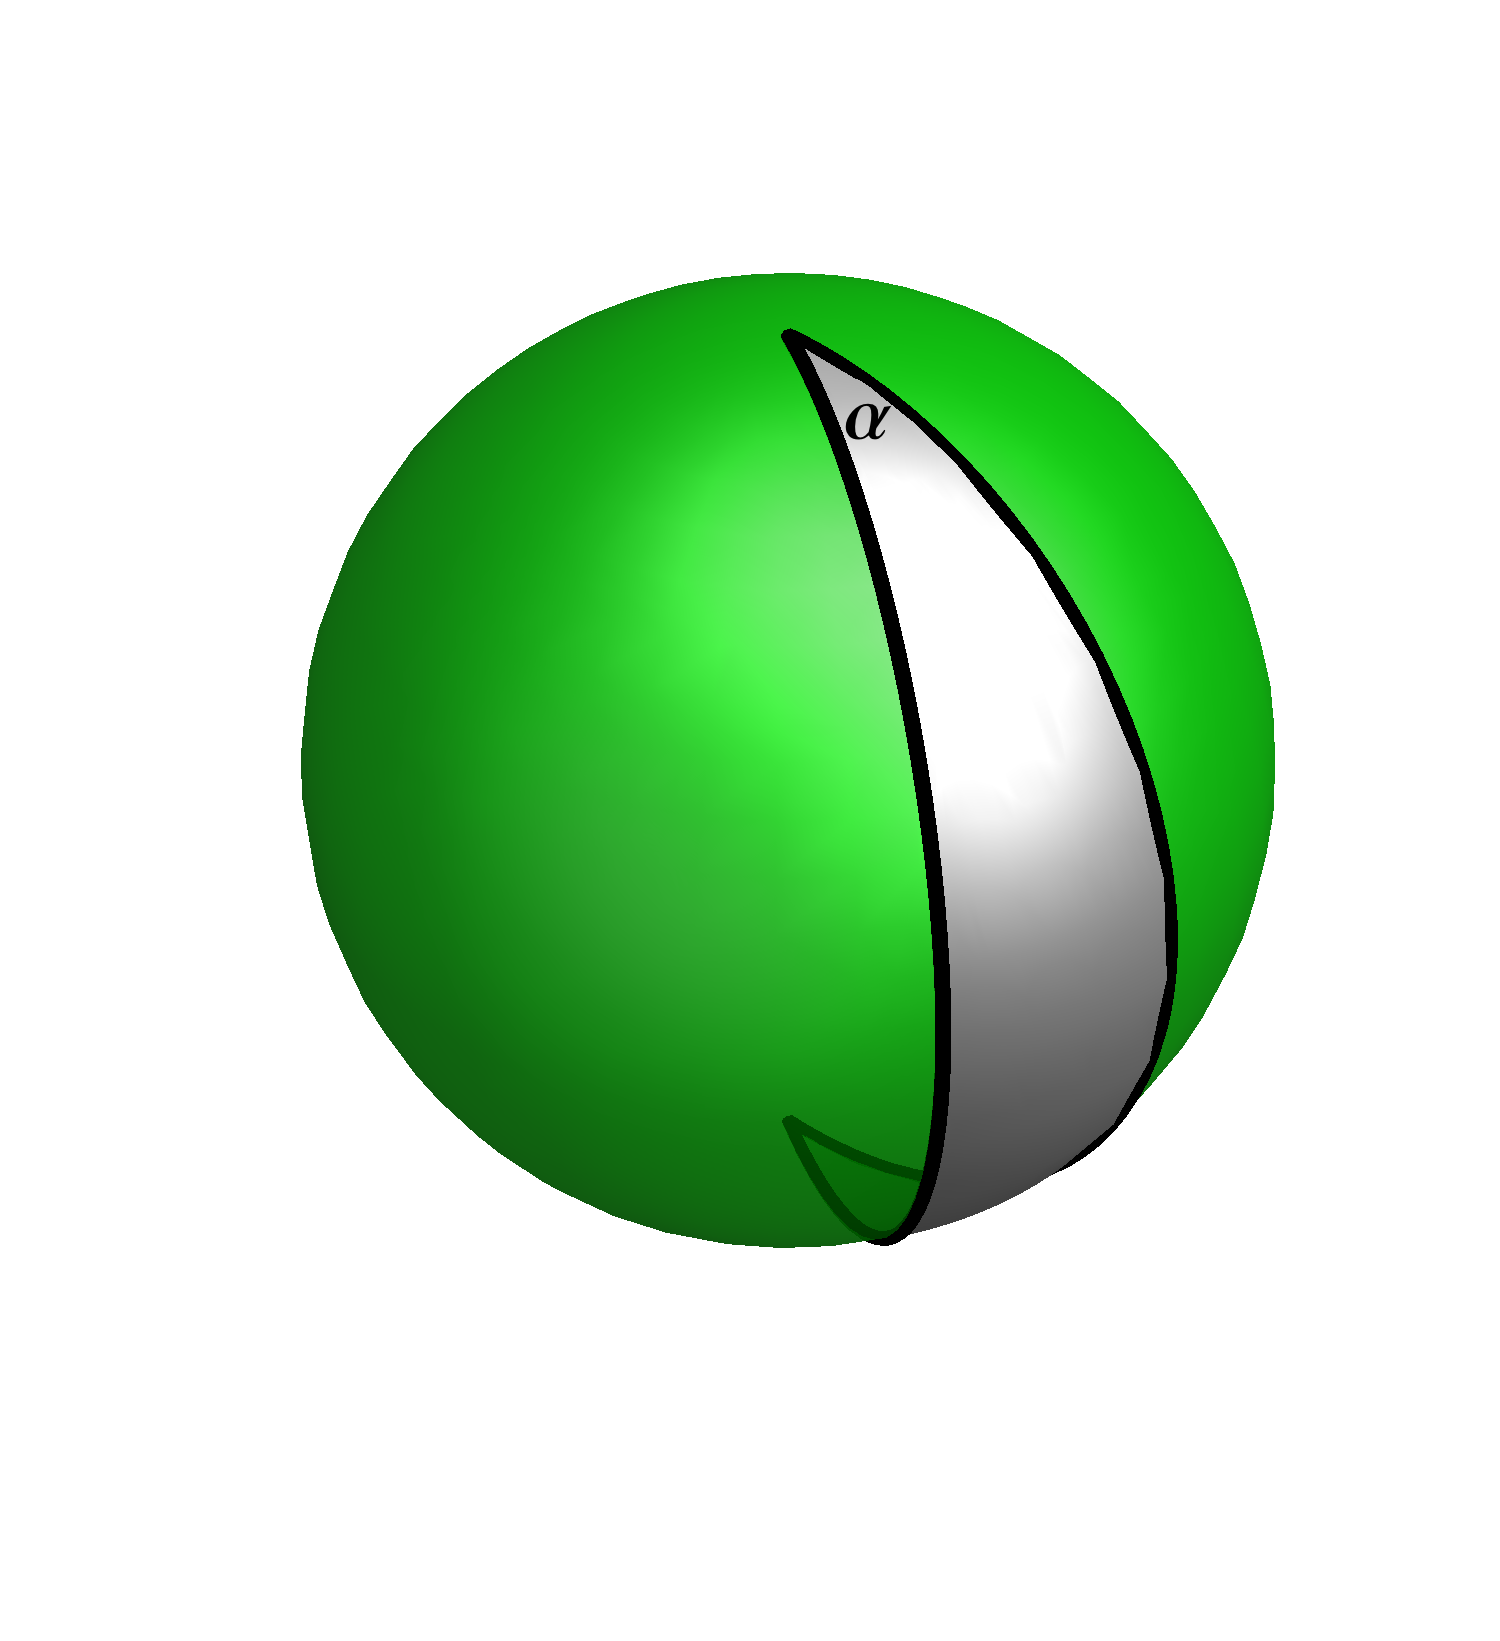
\includegraphics[width=3in]{W13_3.png}%
\end{image}


The lune has two vertices. They are at opposite (antipodal) points on the
$R$-sphere, that is, the line in Eucludean $3$-space that joins the two
vertices runs through the center of the sphere. The angle at a vertex of the
lune is $\alpha$ radians.

\begin{exercise}
\label{67} Explain why the area of the $\alpha$-lune is $2\alpha
\cdot R^{2}$.
\end{exercise}


\subsection*{Spherical triangles}

If a triangle on the sphere of radius $R$ has interior angles with radian
measures $\alpha$, $\beta$, and $\gamma$, it can be covered three times by
lunes as shown in the figure below.%
\begin{image}
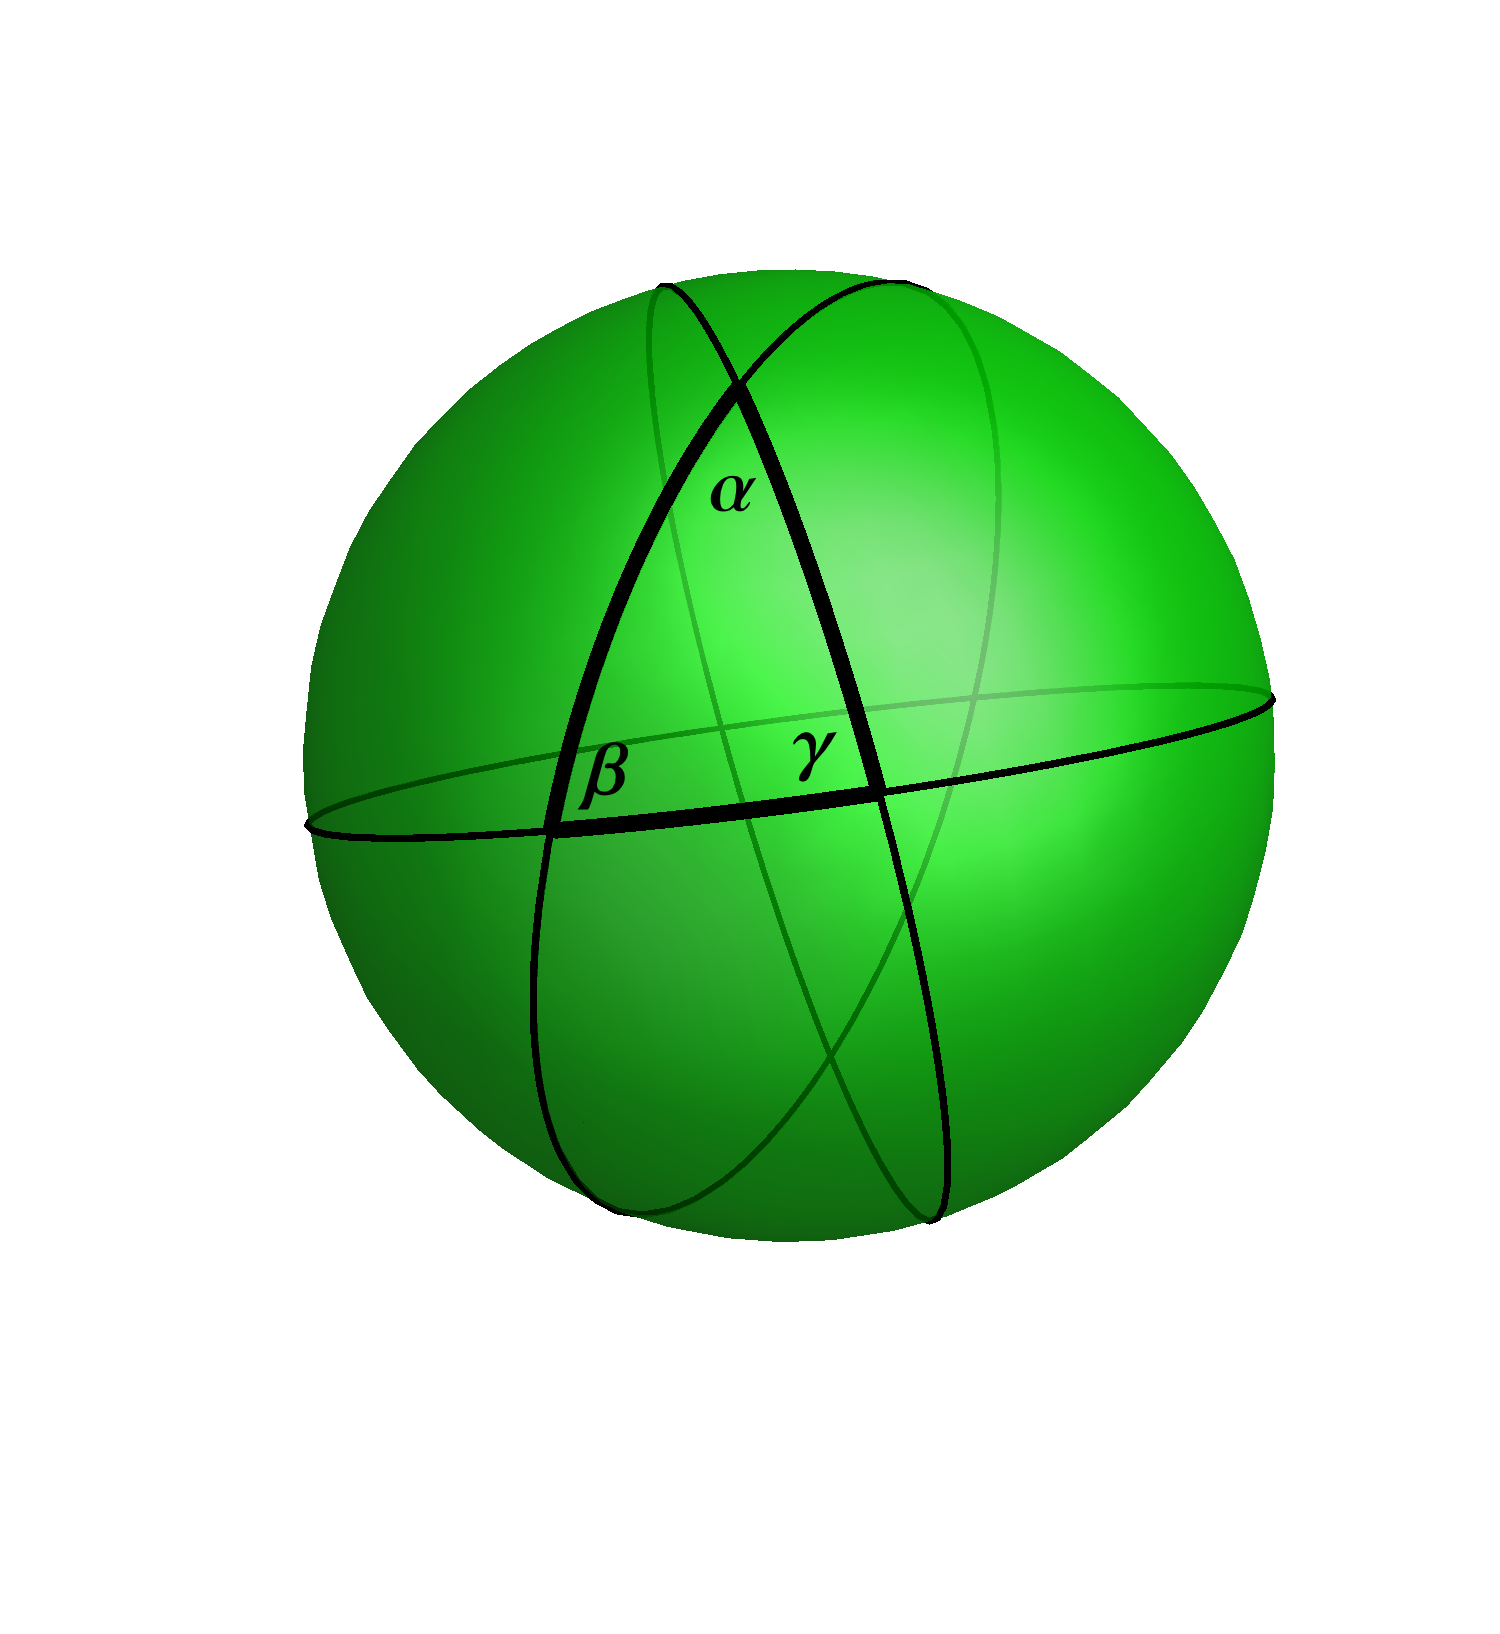
\includegraphics[width=3in]{W13_4.png}%
\end{image}
Notice that each lune has one vertex at a vertex of the triangle and angle
equal to that interior angle of the triangle. The other vertices of each lune
are vertices of an `opposite' triangle that has the same area as the given one
since it is just the image of the given one under the rigid motion%
\[
\left(  \underline{\hat{x}},\underline{\hat{y}},\underline{\hat{z}}\right)
=\left(  \hat{x},\hat{y},\hat{z}\right)  \cdot\left(
\begin{array}
[c]{ccc}%
-1 & 0 & 0\\
0 & -1 & 0\\
0 & 0 & -1
\end{array}
\right)  .
\]
The three lunes cover the triangle three times. The three opposite
lunes cover the opposite triangle three times. If you take all six
lunes together, they cover each of the two triangles three times and
everything else exactly once.

\begin{exercise}\hfil
\begin{enumerate}
\item Show that the area of the spherical triangle is given by the
formula%
\[
R^{2}\left(  \left(  \alpha+\beta+\gamma\right)  -\pi\right).
\]
Hint: Use Exercise \ref{67} to turn the sentence just preceding the Exercise
into an equation.

\item Give a formula for the area of any spherical $n$-gon.

Hint: Divide the spherical $n$-gon into spherical triangles.
\end{enumerate}
\end{exercise}
\end{document}

\documentclass{ximera}

\usepackage{microtype}
\usepackage{tikz}
\usepackage{tkz-euclide}
\usetkzobj{all}
\tikzstyle geometryDiagrams=[ultra thick,color=blue!50!black]

\renewcommand{\epsilon}{\varepsilon}



\title{Euclidean three-space as a metric space}

\begin{document}
\begin{abstract}
In this activity we will work in three dimensional space and see the
importance of the dot product to geometry.
\end{abstract}
\maketitle

\subsection*{Points and vectors in euclidean 3-space}

In this book, we will study all the \textit{two}-dimensional
geometries (spheres, the plane and hyperbolic spaces). Each one of
these geometries looks the same at each of its points and it also
looks the same in every direction emanating from any of its
points. But to study them all at the same time and in a uniform way we
will need to visualize them all as different surfaces lying in some
common \textit{three}-dimensional space. Let's examine this
``ambient'' space.


For those we begin with three-dimensional euclidean space%
\[
\mathbb{R}^{3}=\left\{  \left(  \hat{x},\hat{y},\hat{z}\right)  :\hat{x}%
,\hat{y},\hat{z}\in\mathbb{R}\right\}.
\]
We will want to reserve the notation $\left( x,y,z\right) $ for some
new coordinates that we will put on the `same' objects in the next
section. In euclidean space, there is a standard way to measure distance between two points%
\begin{align*}
\hat{X}_{1}  &  =\left(  \hat{x}_{1},\hat{y}_{1},\hat{z}_{1}\right) \\
\hat{X}_{2}  &  =\left(  \hat{x}_{2},\hat{y}_{2},\hat{z}_{2}\right)  ,
\end{align*}
namely%
\begin{equation}
d\left(  \hat{X}_{1},\hat{X}_{2}\right)  =\sqrt{\left(  \hat{x}_{2}-\hat
{x}_{1}\right)  ^{2}+\left(  \hat{y}_{2}-\hat{y}_{1}\right)  ^{2}+\left(
\hat{z}_{2}-\hat{z}_{1}\right)  ^{2}}. \label{0}%
\end{equation}

When you see $\left( \hat{x},\hat{y},\hat{z}\right)$ in what follows,
that means that distance between points is measured by the formula
above. One more thing, in euclidean three-space it
will be important throughout to make the distinction between
\textbf{points} and \textbf{vectors}: Although each will be
represented by a triple of real numbers we will use%
\[
\hat{X}=\left(  \hat{x},\hat{y},\hat{z}\right)
\]
to denote \textbf{points}, that is, \textbf{position} in euclidean $3$-space,
and%
\[
\hat{V}=\left(  \hat{a},\hat{b},\hat{c}\right)
\]
to denote \textbf{vectors}, that is, \textbf{displacement} by which we mean
the amount and direction a given point is being moved. So vectors always
indicate \textit{motion} from an explicit (or implicit) \textit{point} of
reference. 

\subsection*{The dot product determines length, angle, and area}

There are various operations we can perform on one or more vectors when we
think of them as emanating from the same point in euclidean $3$-space. The
first is the dot product of two vectors.

\begin{definition}
The dot product of two vectors%
\begin{align*}
\hat{V}_{1}  &  =\left(  \hat{a}_{1},\hat{b}_{1},\hat{c}_{1}\right) \\
\hat{V}_{2}  &  =\left(  \hat{a}_{2},\hat{b}_{2},\hat{c}_{2}\right)
\end{align*}
emanating from the same point in 3-dimensional euclidean space is
defined as the real number given by the formula%
\[
\hat{a}_{1}\hat{a}_{2}+\hat{b}_{1}\hat{b}_{2}+\hat{c}_{1}\hat{c}_{2}%
\]
or in matrix notation as%
\[
\begin{bmatrix}
\hat{a}_{1} & \hat{b}_{1} & \hat{c}_{1}%
\end{bmatrix}
\begin{bmatrix}
\hat{a}_{2}\\
\hat{b}_{2}\\
\hat{c}_{2}%
\end{bmatrix}.
\]
It is also denoted as%
\[
\hat{V}_{1}\bullet\hat{V}_{2}%
\]
or in matrix notation as%
\[
\hat{V}_{1}\cdot \hat{V}_{2}^\transpose.
\]

\end{definition}

\begin{problem}
Give the formula for the length $\left\vert \hat{V}\right\vert $ of a vector
$\hat{V}=\left(  \hat{a},\hat{b},\hat{c}\right)  $ in 3-dimensional euclidean
space in terms of dot product.
\end{problem}


\begin{lemma}[Law of Cosines]
\label{110} The (smaller) angle $\theta$ between two
vectors $\hat{V}_{1}$ and $\hat{V}_{2}$ emanating from $O=\left(
0,0,0\right)  $ satisfies the relation%
\[
\left\vert \hat{V}_{2}-\hat{V}_{1}\right\vert ^{2}=\left\vert \hat{V}%
_{1}\right\vert ^{2}+\left\vert \hat{V}_{2}\right\vert ^{2}-2\left\vert
\hat{V}_{1}\right\vert \cdot\left\vert \hat{V}_{2}\right\vert \cdot
\cos\theta.
\]
\end{lemma}

Now we will prove this lemma. Your task is to fill-in the details of
the proof below.

\begin{problem}
Start by noting that without loss of generality we can assume that
$\left\vert \hat{V}% _{1}\right\vert \leq\left\vert
\hat{V}_{2}\right\vert$. Consider the triangle with one side given by
the segment from $O=\left( 0,0,0\right) $ to the endpoint $P_{1}$ of
$\hat{V}_{1}$, with a second side $S_{2}$ given by the segment from
$O$ to the endpoint $P_{2}$ of $\hat{V}_{2}$ and with the third side
given by the segment joining $P_{1}$ and $P_{2}$. Let $P$ be the
point on $S_{2}$ so that the segment between $P_{1}$ and $P$ is
perpendicular to $S_{2}$.
\begin{itemize}
\item Illustrate the diagram described above. 
\end{itemize}

By the Pythagorean theorem%
\begin{align*}
|P_{1}P_{2}|^{2} - |P_{2}P|^{2} &= |PP_{1}|^{2}\\
&= |OP_{1}|^{2} - |OP|^{2}\\
\end{align*}
\begin{itemize}
\item Explain the lines above.
\end{itemize}
\begin{align*}
|P_{1}P_{2}|^{2} &= |OP_{1}|^{2}+\left(|P_{2}P|^{2}-|OP|^{2}\right) \\
&=|OP_{1}|^{2}+\left(|P_{2}P|+|OP|\right)\left(|P_{2}P|-|OP| \right)
\end{align*}
\begin{itemize}
\item Explain the lines above.
\end{itemize}
\begin{align*}
&=|OP_{1}|^{2}+|OP_{2}| \left(|P_{2}P|-|OP|\right)\\
&=|OP_{1}|^{2}+|OP_{2}| \left(|OP_{2}| -2| OP| \right)
\end{align*}
\begin{itemize}
\item Explain the lines above.
\end{itemize}
But%
\[
|OP| =|OP_{1}| \cdot\cos\theta.
\]
\begin{itemize}
\item Explain how this completes the proof.
\end{itemize}
\end{problem}



%% \begin{problem}
%% What can you say about the cosine of the larger of the two angles between two
%% vectors $\hat{V}_{1}$ and $\hat{V}_{2}$, that is about $\left(  360^{\circ
%% }-\theta\right)  $?
%% \end{problem}

\begin{theorem}
\label{111}The angle $\theta$ between two vectors $\hat{V}_{1}$ and
$\hat{V}_{2}$ emanating from the same point in euclidean $3$-space satisfies
the relation
\begin{equation}
\hat{V}_{1}\bullet\hat{V}_{2}=\left\vert \hat{V}_{1}\right\vert \cdot
\left\vert \hat{V}_{2}\right\vert \cdot\cos\theta. \label{2}%
\end{equation}
[DS,30ff]
\end{theorem}

Now we will prove this theorem. Your task is to fill-in the details of
the proof below.

\begin{problem}
Multiplying out using the definition and algebraic properties of dot product,%
\begin{align*}
\left\vert \hat{V}_{2}-\hat{V}_{1}\right\vert ^{2}  &  =\left(  \hat{V}%
_{2}-\hat{V}_{1}\right)  \bullet\left(  \hat{V}_{2}-\hat{V}_{1}\right) \\
&  =\left\vert \hat{V}_{1}\right\vert ^{2}+\left\vert \hat{V}_{2}\right\vert
^{2}-2\left(  \hat{V}_{1}\bullet\hat{V}_{2}\right)  .
\end{align*}
Now apply the previous lemma.

Explain how this proves the theorem. 
\end{problem}

The significance of the theorem above is that the measure of angles between
vectors depends only on the definition of the dot product.

\begin{corollary}
The formula for the angle $\theta$ between two vectors $\hat{V}_{1}=\left(
\hat{a}_{1},\hat{b}_{1},\hat{c}_{1}\right)  $ and $\hat{V}_{2}=\left(  \hat
{a}_{2},\hat{b}_{2},\hat{c}_{2}\right)  $ in $3$-dimensional euclidean space
depends only on the dot products of the two vectors with themselves and with
each other. Namely%
\[
\theta=\arccos\left(  \frac{\hat{V}_{1}\bullet\hat{V}_{2}%
}{\left\vert \hat{V}_{1}\right\vert \cdot\left\vert \hat{V}_{2}\right\vert
}\right)  .
\]

\end{corollary}

In fact it is also true that the formula for the area of the parallelogram
determined by two vectors $\hat{V}_{1}$ and $\hat{V}_{2}$ depends only on the
dot products of the two vectors with themselves and with each other. You will
see this by answering the following problems.

\begin{problem}
Show that the area of the parallelogram determined by $\hat{V}_{1}$ and
$\hat{V}_{2}$ emanating from the same point in euclidean $3$-space is given by%
\[
|\hat{V}_{1}|\cdot|\hat{V}_{2}|\cdot\sin\theta.
\]
\end{problem}

\begin{problem}
\label{9}Show that the area of the parallelogram determined by $\hat{V}_{1}$
and $\hat{V}_{2}$ emanating from the same point in euclidean $3$-space is also
given by%
\[
\sqrt{\det
\begin{bmatrix}
\hat{V}_{1}\bullet\hat{V}_{1} & \hat{V}_{2}\bullet\hat{V}_{1}\\
\hat{V}_{1}\bullet\hat{V}_{2} & \hat{V}_{2}\bullet\hat{V}_{2}%
\end{bmatrix}}.
\]

\begin{hint}
Start from the square of
$|\hat{V}_{1}|\cdot|\hat{V}_{2}|\cdot\sin\theta$, substitute $\left(
1-\cos^{2}\theta\right)$ for $\sin^{2}\theta$, and use the theorem
above. Alternatively start from
$|\hat{V}_{1}|\cdot|\hat{V}_{2}|\cdot\sin\theta$ and show that%
\[
\sin\left(  \arccos\left(  \frac{\hat{V}_{1}\bullet\hat{V}%
_{2}}{\left\vert \hat{V}_{1}\right\vert \cdot\left\vert \hat{V}_{2}\right\vert
}\right)  \right)  
=\frac{\sqrt{\det
    \begin{bmatrix}
      \hat{V}_{1}\bullet\hat{V}_{1} & \hat{V}_{2}\bullet\hat{V}_{1}\\
      \hat{V}_{1}\bullet\hat{V}_{2} & \hat{V}_{2}\bullet\hat{V}_{2}
    \end{bmatrix}
  }
}{\left\vert\hat{V}_{1}\right\vert \cdot\left\vert
  \hat{V}_{2}\right\vert }.
\]
\end{hint}

\end{problem}

\begin{problem}
Show that we have the following equality of matrices%
\[
\begin{bmatrix}
\hat{V}_{1}\bullet\hat{V}_{1} & \hat{V}_{2}\bullet\hat{V}_{1}\\
\hat{V}_{1}\bullet\hat{V}_{2} & \hat{V}_{2}\bullet\hat{V}_{2}%
\end{bmatrix}
=
\begin{bmatrix}
\hat{V}_{1} \\
\hat{V}_{2}
\end{bmatrix}
\cdot
\begin{bmatrix}
\hat{V}_{1}^\transpose  & \hat{V}_{2}^\transpose 
\end{bmatrix}.
\]

\end{problem}

Again, the significance of the previous problems is that, to compute
areas, we only need to know how to compute dot-products. Hence, it is
the definition of the dot-product of the vectors completely determines
the calculation of the area of the parallelogram they generate.  We
finish this section with one other related fact.

\begin{lemma}
The area of the parallelogram determined by two vectors $\hat{V}_{1}=\left(
\hat{a}_{1},\hat{b}_{1},\hat{c}_{1}\right)  $ and $\hat{V}_{2}=\left(  \hat
{a}_{2},\hat{b}_{2},\hat{c}_{2}\right)  $ emanating from the same point in
euclidean $3$-space is given by the length of the cross-product%
\[
\hat{V}_{1}\times\hat{V}_{2}=\left(
\det\begin{bmatrix}
\hat{b}_{1} & \hat{c}_{1}\\
\hat{b}_{2} & \hat{c}_{2}%
\end{bmatrix},
\det\begin{bmatrix}
\hat{c}_{1} & \hat{a}_{1}\\
\hat{c}_{2} & \hat{a}_{2}%
\end{bmatrix},
\det\begin{bmatrix}
\hat{a}_{1} & \hat{b}_{1}\\
\hat{a}_{2} & \hat{b}_{2}%
\end{bmatrix}
\right).
\]

\end{lemma}

Now we will prove this lemma. Your task is to fill-in the details of
the proof below.

\begin{problem}
We use some facts from linear algebra. First of all, develop the determinant%
\[
\det
\begin{bmatrix}
\hat{V}_{1} \\
\hat{V}_{2} \\
\hat{V}_{1}\times\hat{V}_{2}
\end{bmatrix}
\]
along the third row.
\begin{itemize}
\item Conclude that 
\[
\left\vert
\det
\begin{bmatrix}
\hat{V}_{1} \\
\hat{V}_{2} \\
\hat{V}_{1}\times\hat{V}_{2}
\end{bmatrix}\right\vert
=\left\vert \hat{V}_{1}\times\hat{V}_{2}\right\vert ^{2}
\]
\item On the other hand by developing the left-hand determinant along
  the third row, show that
\[
\det
\begin{bmatrix}
\hat{V}_{1} \\
\hat{V}_{2} \\
\hat{V}_{1}
\end{bmatrix}
=0
\]
\end{itemize}
Hence we conclude that $\hat{V}_{1}$ is perpendicular to
$\hat{V}_{1}\times\hat{V}_{2}$. Similarly $\hat{V}_{2}$ is
perpendicular to $\hat{V}_{1}\times\hat{V}_{2}$. Finally, the absolute
value of the determinant of a $3\times3$ matrix%
\[
\left\vert
\det
\begin{bmatrix}
\hat{V}_{1} \\
\hat{V}_{2} \\
\hat{V}_{1}\times\hat{V}_{2}
\end{bmatrix}
\right\vert
\]
is the volume of the parallelepiped determined by the row vectors of the
matrix. But that volume is%
\[
\left( \left\vert \hat{V}_{1}\right\vert \cdot\left\vert \hat{V}%
_{2}\right\vert \cdot\sin\theta\right)  \cdot\left\vert \hat{V}%
_{1}\times\hat{V}_{2}\right\vert
\]
since $\left(  \left\vert \hat{V}_{1}\right\vert \cdot\left\vert \hat{V}%
_{2}\right\vert \cdot\sin\theta\right)  $ is the area of the base
of the parallelepiped and $\hat{V}_{1}\times\hat{V}_{2}$ is perpendicular to
both $V_{1}$ and $V_{2}$. So we see
\[
\left(  \left\vert \hat{V}_{1}\right\vert \cdot\left\vert \hat{V}%
_{2}\right\vert \cdot\sin\theta\right)  \cdot\left\vert \hat{V}%
_{1}\times\hat{V}_{2}\right\vert =\left\vert
\det\begin{bmatrix}
\hat{V}_{1} \\
\hat{V}_{2} \\
\hat{V}_{1}\times\hat{V}_{2}
\end{bmatrix}
\right\vert =\left\vert \hat{V}_{1}\times\hat{V}_{2}\right\vert ^{2}.
\]
So%
\[
\left(  \left\vert \hat{V}_{1}\right\vert \cdot\left\vert \hat{V}%
_{2}\right\vert \cdot\sin\theta\right)  =\left\vert \hat{V}%
_{1}\times\hat{V}_{2}\right\vert .
\]
%[DS,42-47]
\begin{itemize}
\item Explain how this completes the proof. 
\end{itemize}
\end{problem}


\subsection*{Curves in euclidean $3$-space and vectors tangent to them}

\begin{definition}
A \textbf{smooth curve in }$\mathbf{3}$\textbf{-dimensional euclidean space}
is given by a differentiable mapping%
\begin{gather*}
\hat{X}:\left[  b,e\right]  \rightarrow\mathbb{R}^{3}\\
t\mapsto\left(  \hat{x}\left(  t\right)  ,\hat{y}\left(  t\right)  ,\hat
{z}\left(  t\right)  \right)
\end{gather*}
from an interval $\left[ b,e\right] $ on the real line. We shall
sometimes use the notation%
\[
\left(  \hat{x}\left(  t\right)  ,\hat{y}\left(  t\right)  ,\hat{z}\left(
t\right)  \right)  =\hat{X}\left(  t\right)  .
\]
The mapping $\hat{X}\left(  t\right)  $ must have the additional property that
the tangent vector
\[
\left(  \hat{a}\left(  t\right)  ,\hat{b}\left(  t\right)  ,\hat{c}\left(
t\right)  \right)  =\left(  \frac{d\hat{x}}{dt},\frac{d\hat{y}}{dt}%
,\frac{d\hat{z}}{dt}\right)  =\frac{d\hat{X}}{dt}%
\]
is not the zero vector for any $t$ in $\left[ b,e\right] $.
\end{definition}

\begin{problem}\hfil
\begin{enumerate}
\label{1}\item Give two examples of smooth curves,
\begin{align*}
\hat{X}_{1}\left(  s\right)   &  =\left(  \hat{x}_{1}\left(  s\right)
,\hat{y}_{1}\left(  s\right)  ,\hat{z}_{1}\left(  s\right)  \right) \\
\hat{X}_{2}\left(  t\right)   &  =\left(  \hat{x}_{2}\left(  t\right)
,\hat{y}_{2}\left(  t\right)  ,\hat{z}_{2}\left(  t\right)  \right)
\end{align*}
neither of which is a straight line, in $3$-dimensional euclidean space. Do
this so that the two curves pass through a common point and go in distinct
tangent directions at that point. Please choose curves so that none of the
coordinate functions of $s$ or $t$ is a constant function. [DS,71ff]

\item Compute the tangent vectors of each of the two curves at each of their points.

\item For the two curves you defined in a), what are the coordinates of the point
in euclidean $3$-space at which the two curves intersect?

\item Use the dot product formula to compute the angle $\theta$ between (the
tangent vectors to) your two example curves in a) at the point at which the
curves intersect. [DS,20-21]
\end{enumerate}
\end{problem}

Sometimes displacement is measured by showing how a given point is displaced,
as in%
\[
\hat{V}=\hat{X}_{2}-\hat{X}_{1}=\left(  \hat{x}_{2}-\hat{x}_{1},\hat{y}%
_{2}-\hat{y}_{1},\hat{z}_{2}-\hat{z}_{1}\right)  ,
\]
and sometimes displacement is expressed as the instantaneous velocity of a
point moving along a curve as in%
\[
\hat{V}=\frac{d\hat{X}\left(  t\right)  }{dt}=\left(  \frac{d\hat{x}\left(
t\right)  }{dt},\frac{d\hat{y}\left(  t\right)  }{dt},\frac{d\hat{z}\left(
t\right)  }{dt}\right)  .
\]
[DS,30ff].

In matrix notation we can think of
\[
\hat{X}_{2}-\hat{X}_{1}=\left(  \hat{x}_{2}-\hat{x}_{1},\hat{y}_{2}-\hat
{y}_{1},\hat{z}_{2}-\hat{z}_{1}\right)
\]
as a $1\times3$ matrix $\left[\hat{X}_{2}-\hat{X}_{1}\right]$. Then we can
write the formula for the distance between two points $\hat{X}_{1}$ and
$\hat{X}_{2}$ in euclidean $3$-space in terms of the dot-product%
\begin{equation}
d\left(  \hat{X}_{1},\hat{X}_{2}\right)  =\sqrt{\left(  \hat{X}_{2}-\hat
{X}_{1}\right)  \bullet\left(  \hat{X}_{2}-\hat{X}_{1}\right)  } \label{13}%
\end{equation}
or in terms of the matrix product%
\[
d\left( \hat{X}_{1},\hat{X}_{2}\right) =\sqrt{\left[
  \hat{X}_{2}-\hat{X}_{1} \right] \cdot\left[\hat{X}_{2}-\hat{X}%
  _{1}\right]^\transpose }.
\]


\subsection*{Length of a smooth curve in euclidean $3$-space}

\begin{problem}
Compute the length of the tangent vector
\[
\l(t)=\sqrt{\frac{d\hat{X}}{dt}\bullet\frac{d\hat{X}}{dt}}%
\]
to each of your two example curves in the previous problem at each of
their points.
\end{problem}

\begin{definition}
The length $L$ of the curve $\hat{X}(t)$, $t\in[b,e] $, in euclidean
$3$-space is obtained by integrating the length of the tangent vector
to the curve, that is,%
\[
L=\int_{b}^{e} \l(t)  \,dt.
\]
[DS,82] Notice that the length of any curve only depends on the definition of
the dot-product. That is, if we know the formula for the dot-product, we know
(the formula for) the length of any curve.
\end{definition}

Our first example is the path%
\begin{align*}
\left(  \hat{x}\left(  t\right)  ,\hat{y}\left(  t\right)  ,\hat{z}\left(
t\right)  \right)   &  =\left(  R\cdot \sin\left(  t\right)  ,0,R\cdot
\cos\left(  t\right)  \right) \label{6}\\
0\,  &  \leq t\leq\pi.
\end{align*}


Notice that this path lies on the sphere of radius $R$.

\begin{problem}
Write the formula for the tangent vector to the path above at each
point using
$\left(\hat{x}(t),\hat{y}(t),\hat{z}(t)\right)$-coordinates. Show that
the length of this path is $R\pi$.
\end{problem}

\begin{problem}
Compute the length of each of your two example curves in the previous
problem.
\end{problem}

\begin{remark}
In this last problem, you may easily be confronted with an integral
that you cannot compute. For example, if your curve $\hat{X}_{1}\left(
t\right) $ happens to describe an ellipse that is not circular, it was
proved in the 19th century that no formula involving only the
standard functions from calculus will give you the length of your path
from a fixed beginning point to a variable ending point on the
ellipse. If that kind of thing occurs, go back and change the
definitions of your curves in the previous problem until you get two
curves for which you can compute length of your path from a fixed
beginning point to a fixed ending point. [DS,81-82]
\end{remark}




We want to extend such ideas to objects like spheres
\[
\left\{  \left(  \hat{x},\hat{y},\hat{z}\right)  \in\mathbb{R}^{3}:\hat{x}%
^{2}+\hat{y}^{2}+\hat{z}^{2}=R^{2}\right\}
\]
of a fixed radius $R$, since these can be faithfully represented in
ordinary euclidean three-space.  However, there is one disconcerting
fact: As $R$ approaches infinity, the geometry of the $R$-sphere at
any point looks more and more like plane geometry, but on the other
hand, that `limit' plane geometry is `out at infinity.' 

To study all the two-dimensional geometries, including plane geometry
and the hyperbolic geometries, in a uniform way we will have to
\textit{change} the coordinate system we use, or, what will turn out
to be the same thing, we will have to change the distance formula
slightly for each geometry. In fact this means we will change
coordinates.  These new coordinates will be chosen to keep the north
and south poles from going to infinity as the radius $R$ of a sphere
increases without bound. This change of viewpoint will eventually let
us go non-euclidean or, in the language of Buzz Lightyear ``to
infinity and beyond.'' The idea will be like the change from
rectangular to polar coordinates for the plane that you encountered in
calculus, only easier.


\begin{problem}
Summarize the results from this section. In particular, indicate which
results follow from the others.
\begin{freeResponse}
\end{freeResponse}
\end{problem}

\end{document}

\documentclass[newpage,hints,handout]{ximera}

\usepackage{microtype}
\usepackage{tikz}
\usepackage{tkz-euclide}
\usetkzobj{all}
\tikzstyle geometryDiagrams=[ultra thick,color=blue!50!black]

\renewcommand{\epsilon}{\varepsilon}



\title{Changing coordinates}
\begin{document}
\begin{abstract}
Now we will change coordinates.
\end{abstract}
\maketitle


\section{Bringing the North Pole of the $R$-sphere to $\left(
0,0,1\right)  $}

We are now ready to change coordinates on euclidean $3$-space so that we can fill
up that space  with plane geometry and all the spherical and hyperbolic
geometries.  We have reserved the notation $(x,y,z)$ for these new coordinates
that we will put on the `same' objects we have been studying in euclidean
$(\hat{x},\hat{y},\hat{z})$-coordinates. These new coordinates will be chosen to
keep the north and south poles from going to infinity as the radius $R$ of a
sphere increases without bound. In these now $(x,y,z)$-coordinates the sphere of
radius $R$ will be given by the equation
\[
K(x^{2}+y^{2})+z^{2}=1
\]
where $K=1/R^2$. Notice that the above equation has solutions even when $K$ is negative. It is on those solution sets that hyperbolic geometries will live. So this change of
viewpoint will eventually let us go hyperbolic or, in the language of Buzz
Lightyear, will let $R$ go `to infinity and beyond.' The
idea will be like the change from rectangular to polar coordinates for the
plane that you encountered in calculus, only easier. 

We are now ready to introduce this slightly different set of coordinates for
$\mathbb{R}^{3}$, three-dimensional euclidean space. To understand a bit better why we are doing this,
suppose we are standing at the North Pole%
\[
N=(0,0,R)
\]
of the sphere%
\[
\hat{x}^{2}+\hat{y}^{2}+\hat{z}^{2}=R^{2} %\label{4}%
\]
of radius $R$. As $R$ increases, but we stay our same size, the sphere
around us becomes more and more like a flat, plane surface. However it
can never get completely flat because we are zooming out the positive
$\hat{z}$-axis and we would have to be `at infinity' for our surface
to become exactly flat. We remedy that unfortunate situation by
considering another copy of $\mathbb{R}^{3}$, that we will call
\dfn{$\boldsymbol{K}$-warped space}, whose coordinates we denote as
$\left( x,y,z\right) $.  We make the following rule in order to pass
between the two $\mathbb{R}^{3}$'s:%
\begin{align*}
\hat{x}  &  =x\\
\hat{y}  &  =y\\
\hat{z}  &  =Rz.
\end{align*}
We think of the $\left( x,y,z\right) $-coordinates as simply being a
different set of addresses for the points in euclidean space. For
example,
\[
\left(x,y,z\right)  =\left(0,0,1\right)
\]
tells me that the point in euclidean space that I'm referring to is%
\[
\left(\hat{x},\hat{y},\hat{z}\right) =\left( 0,0,R\right)= N.
\]
Continuing with this ``change of addresses'' the sphere of radius $R$
in euclidean space is given by
\begin{align*}
R^{2} & =\hat{x}^{2}+\hat{y}^{2}+\hat{z}^{2}\\ &
=x^{2}+y^{2}+R^{2}z^{2}
\end{align*}
that is, by the equation
\[
1=\frac{1}{R^{2}}\left(  x^{2}+y^{2}\right)  +z^{2}. %\label{5}%
\]
\begin{definition}
  For the surface defined by
  \[
  1=\frac{1}{R^{2}}\left(  x^{2}+y^{2}\right)  +z^{2}. %\label{5%}
  \]
The quantity $K=\frac{1}{R^{2}}$ is called the \dfn{curvature} of the
$R$-sphere.
\end{definition}

\begin{problem}
  What happens to the surface when $K$ goes to $0$?  How does this relate to the
  colloquial sense of ``curvature''?
  
\begin{freeResponse}
When K goes to zero the surface goes to $z^{2} =1$.  A large sphere is not as curvy as a smaller sphere. As the radius increases, the surface gets flatter so the curvature gets smaller and vice versa.  When the curvature goes to zero, the surface becomes two copies of the plane which makes sense because a plane has zero curvature.  
\end{freeResponse}

\end{problem}

\begin{problem}\hfil
\begin{enumerate}
\item Sketch the solution set in $\left(  x,y,z\right)  $-coordinates
representing the sphere%
\[
R^{2}=\hat{x}^{2}+\hat{y}^{2}+\hat{z}^{2}=1.
\]

\item Sketch the solution set in $\left(  x,y,z\right)  $-coordinates
representing the sphere%
\[
R^{2}=\hat{x}^{2}+\hat{y}^{2}+\hat{z}^{2}=10^{2}.
\]

\item Sketch the solution set in $\left(  x,y,z\right)  $-coordinates
representing the sphere%
\[
R^{2}=\hat{x}^{2}+\hat{y}^{2}+\hat{z}^{2}=10^{-2}.
\]
\end{enumerate}
%
%\begin{hint}
%curvatureOfRsphere Geogebra
%\end{hint}
\end{problem}

\section{Formulas for euclidean lengths, angles, and areas in terms of $(x,y,z)$-coordinates}

To prepare ourselves to do hyperbolic geometry, which (in some sense)
has no satisfactory model in euclidean space, we will `practice' by
doing spherical geometry (which \textit{does} have a completely
satisfactory model in euclidean space) using these `slightly strange'
$\left( x,y,z\right) $-coordinates. Gradually throughout this course
we will discover that the same rules that govern spherical geometry,
expressed in $\left( x,y,z\right) $-coordinates, also govern flat and
hyperbolic geometry! In all three cases, the surface in $\left(
x,y,z\right) $-coordinates that we will study is%
\[
1=K\left(x^{2}+y^{2}\right)+z^{2} .
\]
If $K>0$, the geometry we will be studying is the geometry of the the
euclidean sphere of radius%
\[
R=\frac{1}{\sqrt{K}}.
\]
If $K=0$ we will be studying flat (plane) geometry. If $K<0$, we will be
studying hyperbolic geometry. 

In short, we want to use $\left(  x,y,z\right)  $-coordinates to compute with,
but we want lengths and angles to be the usual euclidean ones in $\left(
\hat{x},\hat{y},\hat{z}\right)  $-coordinates.

\begin{problem}
  Suppose we have a curve $\hat\gamma$ in euclidean space and we think of it as a
  composition of a curve $\gamma$ in $K$-warped space with a transformation.  In
  other words, we're looking at a diagram
  \[
  \begin{tikzcd}
    t \ar[r,mapsto,"\gamma"] \ar[rr,mapsto,bend right=20,swap,"\hat\gamma"] &  (x(t),y(t),z(t))\ar[r,mapsto,"{\left[\begin{smallmatrix}
            \hat x(x,y,z)\\
            \hat y(x,y,z)\\
            \hat z(x,y,z)
          \end{smallmatrix}\right]}"
    ] & \hat\gamma(t)=(\hat x(t),\hat y(t),\hat z(t))
  \end{tikzcd}
  \]
  Use the chain rule to compute
  \[
  \dd[\hat x]{t}, \qquad \dd[\hat y]{t}, \qquad \dd[\hat z]{t},
  \]
  in terms of $\dd[x]{t}$, $\dd[y]{t}$, $\dd[z]{t}$, $\pp[\hat x]{x}$, $\pp[\hat y]{x}$, $\pp[\hat z]{x}$,
  $\pp[\hat x]{y}$, $\pp[\hat y]{y}$, $\pp[\hat z]{y}$, $\pp[\hat x]{z}$, $\pp[\hat y]{z}$, and $\pp[\hat z]{z}$. 
  \begin{hint}
    Recall that if $F$ is a differentiable function of $x$, $y$, and
    $z$; and if $x$, $y$, and $z$ are all differentiable functions of
    $t$, then the chain rule states
    \[
    \dd[F]{t} = \nabla F \cdot
    \begin{bmatrix}
      \dd[x]{t} & \dd[y]{t} & \dd[z]{t}
    \end{bmatrix}^\transpose.
    \]
  \end{hint}
  \begin{freeResponse}
    Write
    \begin{align*}
      \dd[\hat x]{t} &= \begin{bmatrix} \pp[\hat x]{x} & \pp[\hat x]{y} & \pp[\hat x]{z} \end{bmatrix} \cdot \begin{bmatrix} \dd[x]{t} & \dd[y]{t} & \dd[z]{t} \end{bmatrix}^\transpose
      = \pp[\hat x]{x}\cdot\dd[x]{t} + \pp[\hat x]{y}\cdot\dd[y]{t} + \pp[\hat x]{z}\cdot\dd[z]{t}, \\
      \dd[\hat y]{t} &= \begin{bmatrix} \pp[\hat y]{x} & \pp[\hat y]{y} & \pp[\hat y]{z} \end{bmatrix} \cdot \begin{bmatrix} \dd[x]{t} & \dd[y]{t} & \dd[z]{t} \end{bmatrix}^\transpose
      = \pp[\hat y]{x}\cdot\dd[x]{t} + \pp[\hat y]{y}\cdot\dd[y]{t} + \pp[\hat y]{z}\cdot\dd[z]{t}, \\
      \dd[\hat z]{t} &= \begin{bmatrix} \pp[\hat z]{x} & \pp[\hat z]{y} & \pp[\hat z]{z} \end{bmatrix} \cdot \begin{bmatrix} \dd[x]{t} & \dd[y]{t} & \dd[z]{t} \end{bmatrix}^\transpose
      = \pp[\hat z]{x}\cdot\dd[x]{t} + \pp[\hat z]{y}\cdot\dd[y]{t} + \pp[\hat z]{z}\cdot\dd[z]{t}.
    \end{align*}
  \end{freeResponse}
\end{problem}

\begin{problem}
  With the same setting as in the previous problem, rewrite the result
  of your computation in matrix notation to find $D_K$ such that
\[
\begin{bmatrix}
d\hat{x}/dt \\ d\hat{y}/dt \\ d\hat{z}/dt%
\end{bmatrix}
=D_K \cdot \begin{bmatrix}
dx/dt \\ dy/dt \\ dz/dt
\end{bmatrix}
\]
in terms of $\pp[\hat x]{x}$, $\pp[\hat y]{x}$, $\pp[\hat z]{x}$,
$\pp[\hat x]{y}$, $\pp[\hat y]{y}$, $\pp[\hat z]{y}$, $\pp[\hat x]{z}$,
$\pp[\hat y]{z}$, and $\pp[\hat z]{z}$.

\begin{freeResponse}
\[
\begin{bmatrix}
\frac{d\hat{x}}{dt} & \frac{d\hat{y}}{dt} & \frac{d\hat{z}}{dt}%
\end{bmatrix}
=
\begin{bmatrix}
\frac{dx}{dt} & \frac{dy}{dt} & \frac{dz}{dt}%
\end{bmatrix}\cdot
\begin{bmatrix}
\pp[\hat x]{x} & \pp[\hat y]{x} & \pp[\hat z]{x} \\
\pp[\hat x]{y} & \pp[\hat y]{y} & \pp[\hat z]{y} \\
\pp[\hat x]{z} &\pp[\hat y]{z} & \pp[\hat z]{z}
\end{bmatrix}
\]
\[
D_K = 
\begin{bmatrix}
\pp[\hat x]{x} & \pp[\hat y]{x} & \pp[\hat z]{x} \\
\pp[\hat x]{y} & \pp[\hat y]{y} & \pp[\hat z]{y} \\
\pp[\hat x]{z} &\pp[\hat y]{z} & \pp[\hat z]{z}
\end{bmatrix}
\]

\end{freeResponse}
\end{problem}


\begin{problem}
  Use the previous problems and the relationship between euclidean and
  $(x,y,z)$-coordinates to show that
  \[
  \left[\dd[\hat{\gamma}]{t}\right] =
  \begin{bmatrix}
    1 & 0 & 0\\
    0 & 1 & 0\\
    0 & 0 & R
  \end{bmatrix}\cdot \left[ \dd[\gamma]{t}\right].
  \]
  
\begin{freeResponse}
Since we have 
\begin{align*}
\hat{x}  &  =x\\
\hat{y}  &  =y\\
\hat{z}  &  =Rz
\end{align*}
then, 
\[
D_K = 
 \begin{bmatrix}
    1 & 0 & 0\\
    0 & 1 & 0\\
    0 & 0 & R
  \end{bmatrix}.
  \]
  Therefore, 
  \[
 \left[\dd[\hat{\gamma}]{t}\right] 
= \begin{bmatrix}
\frac{d\hat{x}}{dt} & \frac{d\hat{y}}{dt} & \frac{d\hat{z}}{dt}%
\end{bmatrix}
= \left[ \dd[\gamma]{t}\right] \cdot
  \begin{bmatrix}
    1 & 0 & 0\\
    0 & 1 & 0\\
    0 & 0 & R
  \end{bmatrix}.
\]
\end{freeResponse}

\end{problem}

This last computation shows that if
\[
\hat{\mathbf v}_{1}=\begin{pmatrix}\hat{a}_{1} \\ \hat{b}_{1} \\ \hat{c}_{1}\end{pmatrix}
\qquad\text{and}\qquad
\hat{\mathbf v}_{2} =\begin{pmatrix}\hat{a}_{2} \\ \hat{b}_{2} \\ \hat{c}_{2}\end{pmatrix}
\]
are vectors tangent to a curve in $(\hat{x},\hat{y},\hat{z})$-coordinates and
\[
\mathbf{v}_{1}=\begin{pmatrix}a_{1} \\ b_{1} \\ c_{1}\end{pmatrix}
\qquad\text{and}\qquad
\mathbf{v}_{2} =\begin{pmatrix}a_{2} \\ b_{2} \\ c_{2}\end{pmatrix}
\]
are their transformations into $(x,y,z)$-coordinates, then
\[
\hat{\mathbf v}_{1}=
\begin{bmatrix}
1 & 0 & 0\\
0 & 1 & 0\\
0 & 0 & R
\end{bmatrix}\mathbf{v}_{1}
\qquad\text{and}\qquad
\hat{\mathbf v}_{2}=
\begin{bmatrix}
1 & 0 & 0\\
0 & 1 & 0\\
0 & 0 & R
\end{bmatrix}\mathbf{v}_{2} 
\]
and%
\begin{align*}
\hat{\mathbf v}_{1}\bullet\hat{\mathbf v}_{2}
=\hat{\mathbf v}_{1}^\transpose \cdot \hat{\mathbf v}_{2} 
&= 
\left(\begin{bmatrix}
1 & 0 & 0\\
0 & 1 & 0\\
0 & 0 & R
\end{bmatrix}\mathbf{v}_{1}\right)^\transpose
\left(
\begin{bmatrix}
1 & 0 & 0\\
0 & 1 & 0\\
0 & 0 & R
\end{bmatrix}\mathbf{v}_{2}\right)\\
&=\mathbf{v}_{1}^\transpose
\begin{bmatrix}
1 & 0 & 0\\
0 & 1 & 0\\
0 & 0 & R
\end{bmatrix}
\begin{bmatrix}
1 & 0 & 0\\
0 & 1 & 0\\
0 & 0 & R
\end{bmatrix}
\mathbf{v}_{2}\\
&=\mathbf{v}_{1}^\transpose
\begin{bmatrix}
1 & 0 & 0\\
0 & 1 & 0\\
0 & 0 & K^{-1}%
\end{bmatrix}
\mathbf{v}_{2}.
\end{align*}
Hence:
\begin{center}
\textbf{We can compute the euclidean dot product without ever referring to euclidean coordinates!}
\end{center}
We incorporate that fact into the following definition.

\begin{definition}
The \textbf{$\boldsymbol{K}$-dot-product} of vectors:%
\begin{align*}
\mathbf{v}_{1}\bullet_{K}\mathbf{v}_{2}  &=\mathbf{v}_{1}^\transpose
\begin{bmatrix}
1 & 0 & 0\\
0 & 1 & 0\\
0 & 0 & K^{-1}%
\end{bmatrix}
\mathbf{v}_{2}\\
&=
\begin{bmatrix}
a_{1} & b_{1} & c_{1}%
\end{bmatrix}
\begin{bmatrix}
1 & 0 & 0\\
0 & 1 & 0\\
0 & 0 & K^{-1}%
\end{bmatrix}
\begin{bmatrix}
a_{2}\\
b_{2}\\
c_{2}%
\end{bmatrix}.
\end{align*}

\end{definition}

\subsection{Computing length}

\begin{problem}
  Show that if a vector is given to us in $(x,y,z)$-coordinates as%
\[
\mathbf{v}=(a,b,c)^\transpose,
\]
then the length of its image in euclidean space is given by
\[
|\mathbf{v}|_K=\sqrt{\mathbf{v} \bullet_K \mathbf{v}}.
\]

\begin{freeResponse}
$\hat{\mathbf v} = \left(a,b,Rc \right)$ is the image of $V$ in euclidean space. Then,
\begin{align*}
|V|_K = |\hat{\mathbf v}| = \sqrt{\hat{\mathbf v}\bullet\hat{\mathbf v}} 
&= \sqrt{a^{2} + b^{2} + R^{2}c^{2}} \\
&= \begin{bmatrix}
a & b & c%
\end{bmatrix}
\begin{bmatrix}
1 & 0 & 0\\
0 & 1 & 0\\
0 & 0 & K^{-1}%
\end{bmatrix}
\begin{bmatrix}
a\\
b\\
c%
\end{bmatrix} \\
&= \sqrt{V\bullet_K V}
\end{align*}
\end{freeResponse} 
\end{problem}

\begin{problem}
  Consider all vectors in $K$-warped space with their tips on the surface
  \[
  1=K(x^2+y^2)+z^2
  \]
  and their tails at the origin. What can you say about the length of these
  vectors? What does this tell you about the surface for all values of $K>0$?
  
\begin{freeResponse}
Let $V = \left(x,y,z\right)$ be a vector with its tail at the origin and tip on the surface above. Now write the equation of the surface as,
\begin{align*}
\frac{1}{K} &= x^{2} + y^{2} + \frac{1}{K} \cdot z^{2} \\
&= \begin{bmatrix}
	x & y & z
	\end{bmatrix}
\begin{bmatrix}
	1 & 0 & 0 \\
	0 & 1 & 0 \\
	0 & 0 & K^{-1}
	\end{bmatrix}
\begin{bmatrix}
	x \\
	y \\
	z
	\end{bmatrix}\\
&= V \bullet_{K} V
\end{align*}
Then $|V|_{K} = \sqrt{V \bullet_{K} V} = \frac{1}{\sqrt{K}} = |R|$. This tells us that for all values of $K$, except $K=0$, the surface is a sphere. 
\end{freeResponse}

\end{problem}

%% So, suppose we have a curve on the $R$-sphere in euclidean space
%% but it is given to us in $X(t)=(x(t),y(t),z(t))$-coordinates. Then the
%% length of that curve in euclidean space is
%% \[
%% \int_{b}^{e}\sqrt{\frac{dX}{dt}\bullet_{K}\frac{dX}{dt}}\,dt.
%% \]


\subsection{Computing angles}

\begin{problem}
  Show that when $K>0$ if two vectors are given to us in $(x,y,z)$-coordinates as
  \[
  \mathbf{v}_{1}=\begin{pmatrix}a_{1} \\ b_{1} \\ c_{1}\end{pmatrix}
  \qquad\text{and}\qquad
  \mathbf{v}_{2} =\begin{pmatrix}a_{2} \\ b_{2} \\ c_{2}\end{pmatrix}
  \]
  then the angle between their image in euclidean space is given by
  \[
  \theta = \arccos\left(\frac{\mathbf{v}_1\bullet_K \mathbf{v}_2}{|\mathbf{v}_1|_K \cdot|\mathbf{v}_2|_K }\right).
  \]

%angleBetweenVectorsKDotProduct Geogebra%

\begin{freeResponse} Using the previous problems,
\[
\arccos\left(\frac{\mathbf{v}_1\bullet_K \mathbf{v}_2}{\left| \mathbf{v}_1\right|_K \cdot\left|\mathbf{v}_2\right|_K }\right) = \arccos\left(\frac{\hat{\mathbf v}_{1}\bullet \hat{\mathbf v}_{2}}{\left| \hat{\mathbf v}_{1}\right| \cdot\left|\hat{\mathbf v}_{2}\right| }\right) = \theta.
\]
\end{freeResponse}
\end{problem}




\subsection{Computing area}

\begin{problem}
%% Show that, if we have any two vectors in euclidean three-space that
  %% are tangent to the $R$-sphere at some point on it, but the
  
  Show that if two vectors are given to us in $(x,y,z)$-coordinates as
  \[
  \mathbf{v}_{1}=\begin{pmatrix}a_{1} \\ b_{1} \\ c_{1}\end{pmatrix}
  \qquad\text{and}\qquad
  \mathbf{v}_{2} =\begin{pmatrix}a_{2} \\ b_{2} \\ c_{2}\end{pmatrix}
  \]
  then the area of the parallelogram spanned by the image of those two vectors in
  euclidean space is%
  \[
  \sqrt{\det
    \begin{bmatrix}
      \mathbf{v}_{1}\bullet_{K}\mathbf{v}_{1} & \mathbf{v}_{2}\bullet_{K}\mathbf{v}_{1}\\
      \mathbf{v}_{1}\bullet_{K}\mathbf{v}_{2} & \mathbf{v}_{2}\bullet_{K}\mathbf{v}_{2}%
    \end{bmatrix}}
  =\sqrt{\det\left( 
      \begin{bmatrix}
        \mathbf{v}_{1} \\
        \mathbf{v}_{2}
      \end{bmatrix}
      \begin{bmatrix}
        1 & 0 & 0\\
        0 & 1 & 0\\
        0 & 0 & K^{-1}%
      \end{bmatrix}
      \begin{bmatrix}
        \mathbf{v}_{1}^\transpose & \mathbf{v}_{2}^\transpose%
      \end{bmatrix}
    \right) }.
\]

%kCrossProductParallelogram Geogebra%

\begin{freeResponse} In the previous problems it was shown that the K-dot product agrees with the euclidean dot product so, 
\[
\sqrt{\det
\begin{bmatrix}
\mathbf{v}_{1}\bullet_{K}\mathbf{v}_{1} & \mathbf{v}_{2}\bullet_{K}\mathbf{v}_{1}\\
\mathbf{v}_{1}\bullet_{K}\mathbf{v}_{2} & \mathbf{v}_{2}\bullet_{K}\mathbf{v}_{2}%
\end{bmatrix}}
=
\sqrt{\det
\begin{bmatrix}
\hat{\mathbf v}_{1}\bullet \hat{\mathbf v}_{1} & \hat{\mathbf v}_{2}\bullet \hat{\mathbf v}_{1}\\
\hat{\mathbf v}_{1}\bullet \hat{\mathbf v}_{2} & \hat{\mathbf v}_{2}\bullet \hat{\mathbf v}_{2}%
\end{bmatrix}}.
\]
Which was previously shown to be the area of the parallelogram spanned by the image of $\mathbf{v}_1$ and $\mathbf{v}_2$ in euclidean space. To show the equality write,

\begin{align*}
\sqrt{\det
\begin{bmatrix}
\mathbf{v}_{1}\bullet_{K}\mathbf{v}_{1} & \mathbf{v}_{2}\bullet_{K}\mathbf{v}_{1}\\
\mathbf{v}_{1}\bullet_{K}\mathbf{v}_{2} & \mathbf{v}_{2}\bullet_{K}\mathbf{v}_{2}%
\end{bmatrix}}
&=\sqrt{\det
\begin{bmatrix}
a^2_1 + b^2_1 + c^2_1K^{-1} & a_1a_2 + b_1b_2 + c_1c_2K^{-1}\\
a_1a_2 + b_1b_2 + c_1c_2K^{-1} & a^2_2 + b^2_2 + c^2_2K^{-1}%
\end{bmatrix}} \\
&= \sqrt{\det
\begin{bmatrix}
a_{1} & b_{1} & c_{1}\\
a_{2} & b_{2} & c_{2}
\end{bmatrix}
\begin{bmatrix}
1 & 0 & 0\\
0 & 1 & 0\\
0 & 0 & K^{-1}
\end{bmatrix}
\begin{bmatrix}
a_{1} & a_{1}  \\
b_{1} & b_{2}  \\
c_{1} &  c_{2}
\end{bmatrix}} \\
&= \sqrt{\det\left( 
\begin{bmatrix}
\mathbf{v}_{1} \\
\mathbf{v}_{2}
\end{bmatrix}
\begin{bmatrix}
1 & 0 & 0\\
0 & 1 & 0\\
0 & 0 & K^{-1}%
\end{bmatrix}
\begin{bmatrix}
\mathbf{v}_{1}^\transpose & \mathbf{v}_{2}^\transpose%
\end{bmatrix}
\right) }
\end{align*}
\end{freeResponse}

\end{problem}

\textit{Moral of the story:} The dot-product rules! That is, if you
know the dot-product you know everything there is to know about a
geometry, lengths, areas, angles, everything. And the set
\[
1=K\left(x^{2}+y^{2}\right)+z^{2} 
\]
continues to make sense even when $K$ is
negative. And as we will see later on, the definition of the $K$-dot
product also makes sense for tangent vectors to that set when $K$ is
negative. The geometry we get when the constant $K$ is chosen to be
negative is called a hyperbolic geometry. The geometry we get, when
the constant $K$ is just chosen to be non-zero is called a
non-euclidean geometry.  In fact all the non-euclidean $2$-dimensional
geometries are either spherical or hyperbolic.

%% \textit{Coming attractions:} In hyperbolic geometry, when $K^{-1}$ in
%% \[
%% \mathbf{v}_{1}\bullet_{K}\mathbf{v}_{2}  =\mathbf{v}_{1} 
%% \begin{bmatrix}
%% 1 & 0 & 0\\
%% 0 & 1 & 0\\
%% 0 & 0 & K^{-1}%
%% \end{bmatrix}
%% \mathbf{v}_{2}^\transpose
%% \]
%% becomes negative, so that the third coordinate of velocity, that is,
%% the $c$-direction, actually \textit{contracts} lengths. It was the
%% understanding of this mysterious fact that allowed Einstein to
%% discover (special) relativity.


\begin{problem}
Summarize the results from this section. In particular, indicate which
results follow from the others.
\begin{freeResponse}
In this section we started working in $K$-warped space, denoted by $(x, y, z)$-coordinates. We used the following rule to transition between euclidean and  $(x, y, z)$-coordinates:
\begin{align*}
\hat{x}  &  =x\\
\hat{y}  &  =y\\
\hat{z}  &  =Rz.
\end{align*}
In $K$-warped space the following surface,
\[
K\left(x^{2}+y^{2}\right)+z^{2}=1,
\]
 generates the hyperbolic plane when $K<0$, the euclidean plane when $K=0$, and the sphere of radius $R$ when $K> 0$. Using a computation involving the euclidean dot product we defined the $K$-dot-product in $(x, y, z)$-coordinates such that,
\[
\mathbf{v}_{1}\bullet_{K}\mathbf{v}_{2}  = \mathbf{v}_{1} 
\begin{bmatrix}
1 & 0 & 0\\
0 & 1 & 0\\
0 & 0 & K^{-1}%
\end{bmatrix}
\mathbf{v}_{2}^\transpose.
\]
Lastly we calculated formulas for length, area, and the angle between vectors in $(x,y,z)$-coordinates in terms of the $K$-dot-product.
\end{freeResponse}
\end{problem}


\end{document}

\documentclass{ximera}

\usepackage{microtype}
\usepackage{tikz}
\usepackage{tkz-euclide}
\usetkzobj{all}
\tikzstyle geometryDiagrams=[ultra thick,color=blue!50!black]

\renewcommand{\epsilon}{\varepsilon}



\title{Congruences, that is, rigid motions}
\begin{document}
\begin{abstract}
We explore rigid motions as matrix multiplication.
\end{abstract}
\maketitle

\subsection*{Transformations of euclidean space}

Consider the following mapping of euclidean space to itself:%
\[
\begin{bmatrix}
\underline{\hat{x}} & \underline{\hat{y}} & \underline{\hat{z}}%
\end{bmatrix}
=
\begin{bmatrix} \hat{x} & \hat{y} & \hat{z}%
\end{bmatrix}
\cdot\hat{M}
\]
where $\hat{M}$ is an invertible $3\times3$ matrix. Since the matrix
is invertible, this mapping is one-to-one and onto.

\begin{definition}
  A mapping of euclidean space to itself given by
  \[
\begin{bmatrix}
\underline{\hat{x}} & \underline{\hat{y}} & \underline{\hat{z}}%
\end{bmatrix}
=
\begin{bmatrix} \hat{x} & \hat{y} & \hat{z}%
\end{bmatrix}
\cdot\hat{M}
  \]
  is called a \dfn{rigid motion} if the distance between any two
points in euclidean space is left unchanged by the mapping, that is, for
any two points, $\hat{X}_{1}$ and $\hat{X}_{2}$ in euclidean space%
\[
d\left( \hat{X}_{1}  \cdot\hat{M},\hat{X}_{2}
\cdot\hat{M}\right)  =d\left(  \hat{X}_{1},\hat{X}_{2}\right).
\]
\end{definition}

It turns out that there is a special class of matrices that give rise
to rigid motions.

\begin{definition}
  A matrix $\hat{M}$ satisfying
  \[
  \hat{M}\cdot\hat{M}^\transpose=I=\begin{bmatrix}
  1 & 0 & 0\\
  0 & 1 & 0\\
  0 & 0 & 1
  \end{bmatrix}.
  \]
  is called an \dfn{orthogonal} matrix.
\end{definition}

\begin{problem}
  Prove that a matrix $\hat{M}$ defines a rigid motion (a congruence)
  via
  \[
\begin{bmatrix}
\underline{\hat{x}} & \underline{\hat{y}} & \underline{\hat{z}}%
\end{bmatrix}
=
\begin{bmatrix} \hat{x} & \hat{y} & \hat{z}%
\end{bmatrix}
\cdot\hat{M}
  \]
  if and only if it is orthogonal.

  \begin{hint}
    Note that the square of the distance between $\hat{X}_{1}$ and
    $\hat{X}_{2}$ is just the dot-product of the vector%
    \[
    \hat{V}=\hat{X}_{2}-\hat{X}_{1}%
    \]
    with itself. 
  \end{hint}
  \begin{hint}
    If $\hat{M}$ is orthogonal, write
    \[
    \left(  \hat{V}  \cdot\hat{M} \right) \bullet\left(
    \hat{V}  \cdot\hat{M}\right)
    \]
    and deduce that this equals $\hat{V}\bullet\hat{V}$. 
  \end{hint}
  \begin{hint}
  Now suppose that $\hat{M}$ is a rigid motion. Explain why this means that:
  \[
  \left(  \hat{V}  \cdot\hat{M} \right) \bullet\left(
  \hat{V}  \cdot\hat{M}\right)  =\hat{V}\bullet\hat{V}
  \]
  Now rewrite as:
  \[
  \hat{V}\cdot\hat{V}^\transpose= \left(  \hat{V}  \cdot\hat{M} \right) \cdot\left(
    \hat{V}  \cdot\hat{M}\right)^\transpose 
  \]
  \end{hint}
  \begin{hint} Set
    \[
    \hat{V} =
    \begin{bmatrix}
      a & b & c
    \end{bmatrix}
    \]
    and
    \[
    \hat{M} =
    \begin{bmatrix}
      m_{11} & m_{12} & m_{13}\\
      m_{21} & m_{22} & m_{23}\\
      m_{31} & m_{32} & m_{33}
    \end{bmatrix}
    \]
    and view the equation 
    \[
    \hat{V}\cdot\hat{V}^\transpose= \left(  \hat{V}  \cdot\hat{M} \right) \cdot\left(
    \hat{V}  \cdot\hat{M}\right)^\transpose 
    \]
    as an equation of polynomials in the variables $a$, $b$, and $c$. 
  \end{hint}
  \begin{hint}
    Polynomials are equal if and only if their coefficients are equal. 
  \end{hint}
  
  
\begin{freeResponse}
For the first direction we assume that $\hat{M}$ is orthogonal and we want to show that for any two points,  $\hat{X}_{1}$ and $\hat{X}_{2}$,%
\[
   d\left( \hat{X}_{1}  \cdot\hat{M},\hat{X}_{2}
   \cdot\hat{M}\right)  =d\left(  \hat{X}_{1},\hat{X}_{2}\right).
\]
Let $ \hat{V}=\hat{X}_{2}-\hat{X}_{1}$.

\begin{align*}
   d\left( \hat{X}_{1}  \cdot\hat{M},\hat{X}_{2}
   \cdot\hat{M}\right) &= \sqrt{\left(\hat{X}_{2}  \cdot\hat{M}-\hat{X}_{1}  \cdot\hat{M}\right) \bullet \left(\hat{X}_{2}  	\cdot\hat{M}-\hat{X}_{1}  \cdot\hat{M}\right)} \\
   & = \sqrt{\left( \left( \hat{X}_{2}-\hat{X}_{1} \right) \cdot\hat{M}\right) \bullet \left( \left( \hat{X}_{2}-\hat{X}_{1} 		\right) \cdot\hat{M}\right)} \\
   & = \sqrt{ \left(\hat{V}\cdot\hat{M} \right) \bullet \left(\hat{V}\cdot\hat{M} \right)}\\
   & = \sqrt{
       \begin{bmatrix}
          \hat{V}\cdot\hat{M}
       \end{bmatrix} \cdot
       \begin{bmatrix}
          \hat{V}\cdot\hat{M}
       \end{bmatrix}^\transpose}\\
   & = \sqrt{ \hat{V}\cdot\hat{M} \cdot \hat{M}^\transpose \cdot \hat{V}^\transpose} \\
   & = \sqrt{ \hat{V} \cdot \hat{V}^\transpose} \\
   & = \sqrt{\hat{V} \bullet \hat{V}} = \sqrt{d\left(  \hat{X}_{1},\hat{X}_{2}\right)^2} = d\left( \hat{X}_{1},\hat{X}_{2}\right)
\end{align*}

For the other direction we suppose $\hat{M}$ is a rigid motion, so
\[
 d\left( \hat{X}_{1}  \cdot\hat{M},\hat{X}_{2}
   \cdot\hat{M}\right) = d\left(  \hat{X}_{1},\hat{X}_{2}\right).
\]
Therefore, 
\[
	\left(  \hat{V}  \cdot\hat{M} \right) \bullet\left(
    \hat{V}  \cdot\hat{M}\right)  =\hat{V}\bullet\hat{V}.
 \]
Following the hint, write,
\[
\hat{V}\cdot\hat{V}^\transpose= \left(  \hat{V}  \cdot\hat{M} \right) \cdot\left(
    \hat{V}  \cdot\hat{M}\right)^\transpose  = \hat{V} \cdot\hat{M} \cdot \hat{M}^\transpose \cdot \hat{V}^\transpose .
\]
Then, 
\begin{align*}
a^2 + b^2 +c^2
=
\begin{bmatrix}
      a & b & c
    \end{bmatrix}
\begin{bmatrix}
	m_{11} & m_{12} & m_{13}\\
	m_{21} & m_{22} & m_{23}\\
	m_{31} & m_{32} & m_{33}
\end{bmatrix}
\begin{bmatrix}
	m_{11} & m_{21} & m_{31}\\
	m_{12} & m_{22} & m_{32}\\
	m_{13} & m_{23} & m_{33}
\end{bmatrix}
\begin{bmatrix}
      a \\
      b \\
      c
    \end{bmatrix}. \\
 \end{align*}
 Let $\hat{W} = \hat{M} \cdot \hat{M}^\transpose$ then,
 \begin{align*}
 w_{11} &= m_{11}^2 + m_{12}^2 +  m_{13}^2 \\
 w_{12} &= m_{11}m_{21} + m_{12}m_{22} +m_{13}m_{23}\\
 w_{13} &= m_{11}m_{31} + m_{12}m_{32} +m_{13}m_{33}\\
 w_{21} &= m_{21}m_{11} + m_{22}m_{12} +m_{23}m_{13} \\
 w_{22} &= m_{21}^2 + m_{22}^2 +  m_{23}^2 \\
 w_{23} &=  m_{21}m_{31} + m_{22}m_{32} +m_{23}m_{33} \\
 w_{31} &= m_{31}m_{11} + m_{32}m_{12} +m_{33}m_{13} \\
 w_{32} &= m_{31}m_{11} + m_{32}m_{12} +m_{33}m_{13}\\
 w_{33} &= m_{31}^2 + m_{32}^2 +  m_{33}^2.
 \end{align*}    
   
 Since $w_{12} =  w_{21}$, $w_{13} =  w_{31}$, and $w_{23} =  w_{32}$, then 
\[
 a^2 + b^2 +c^2 =  
 \begin{bmatrix}
      a & b & c
    \end{bmatrix} \cdot \hat{W} \cdot \begin{bmatrix}
      a \\
      b \\
      c
    \end{bmatrix} =
a^2 w_{11} + 2abw_{21} + b^2 w_{22} + 2ac w_{13} + c^2 w_{33} + 2bc w_{23}.
\]
Therefore,  $w_{21} =  w_{12} =w_{13} =  w_{31} = w_{23} =  w_{32}=0$, and $w_{11} =  w_{22} =  w_{33}=1$ so $\hat{M}$ is orthogonal. 
 
\end{freeResponse}

\end{problem}


\begin{problem}
  Show that, if $\hat{M}$ is orthogonal, then the transformation
  \[
  \begin{bmatrix}
    \underline{\hat{x}} & \underline{\hat{y}} & \underline{\hat{z}}
  \end{bmatrix}
  =
  \begin{bmatrix}
    \hat{x} & \hat{y} & \hat{z}
  \end{bmatrix}
  \cdot \hat{M}.
  \]
  takes the set of points $\left(\hat{x},\hat{y},\hat{z}\right)$ such
  that
\[
\hat{x}^2 + \hat{y}^2 + \hat{z}^2 = R^2
\]
to the set of points
$\left(\underline{\hat{x}},\underline{\hat{y}},\underline{\hat{z}}\right)$
such that
\[
\underline{\hat{x}}^2 + \underline{\hat{y}}^{2} + \underline{\hat{z}}^{2}=R^2.
\]
That is, $\hat{M}$ gives a one-to-one and onto mapping of the $R$-sphere to
itself.
\begin{hint}
  Write the equation
  \[
  \underline{\hat{x}}^2 + \underline{\hat{y}}^{2} + \underline{\hat{z}}^{2}=R^2
  \]
  as
  \[
  \begin{bmatrix}
    \underline{\hat{x}} & \underline{\hat{y}} & \underline{\hat{z}}%
  \end{bmatrix}  
  \cdot
  \begin{bmatrix}
    \underline{\hat{x}}\\
    \underline{\hat{y}}\\
    \underline{\hat{z}}
  \end{bmatrix}  =R^2.
  \]
\end{hint}

\begin{freeResponse}
\begin{align*}
R^2 = \underline{\hat{x}}^2 + \underline{\hat{y}}^2 +\underline{\hat{z}}^2 
	&= \begin{bmatrix} 
	 \underline{\hat{x}} & \underline{\hat{y}} & \underline{\hat{z}}
  	\end{bmatrix}  
  		\cdot
  	\begin{bmatrix}
    		\underline{\hat{x}}\\
    		\underline{\hat{y}}\\
    		\underline{\hat{z}}
  	\end{bmatrix}\\
	&= \begin{bmatrix} 
		 \underline{\hat{x}} & \underline{\hat{y}} & \underline{\hat{z}}
  		\end{bmatrix}  
  		\cdot
		\begin{bmatrix} 
		 \underline{\hat{x}} & \underline{\hat{y}} & \underline{\hat{z}}
  		\end{bmatrix}^\transpose \\
	&= \begin{bmatrix}
   		 \hat{x} & \hat{y} & \hat{z}
 	        \end{bmatrix}
	       \cdot \hat{M} \cdot \hat{M}^\transpose \cdot 
	      \begin{bmatrix}
	      	{\hat{x}}\\
    		{\hat{y}}\\
    		{\hat{z}}
		\end{bmatrix}\\
	&= \begin{bmatrix}
   		 \hat{x} & \hat{y} & \hat{z}
 	        \end{bmatrix}
	       \cdot
	       \begin{bmatrix}
	      	{\hat{x}}\\
    		{\hat{y}}\\
    		{\hat{z}}
		\end{bmatrix}
	= \hat{x}^2 + \hat{y}^2 + \hat{z}^2 .
\end{align*}
\end{freeResponse}

\end{problem}


\begin{problem}
Explain how the following diagram ``proves'' that functional
composition is \textit{always} associative. Note, we are writing our
functions on the \textit{right} of the argument.
\begin{image}
  \begin{tikzpicture}[scale=.5,geometryDiagrams]

    \node at (-2,8) {$X$};
    \draw[->] (-1.5,8)--(-.5,8);
    \draw[fill=blue!10!white] (0,8) ellipse (0.166 and 0.5);% ellipse
    \draw (.5,7) rectangle (2.5,9);
    \draw (3,8) [partial ellipse=270:450:0.166 and 0.5];
    \node at (1.5,8) {\Large $M_1$};
    \draw (.5,8.5) [partial ellipse=180:270:.5 and 0.166];
    \draw (.5,7.5) [partial ellipse=90:180:.5 and 0.166];
    \draw (2.5,8.5) [partial ellipse=270:360:.5 and 0.166];
    \draw (2.5,7.5) [partial ellipse=0:90:.5 and 0.166];

    %\node at (5,8.6) {$X M_1$};
    \draw[->] (3.5,8)--(6.5,8);
    
    \draw[fill=blue!10!white] (7,8) ellipse (0.166 and 0.5);% ellipse
    \draw (7.5,7) rectangle (9.5,9);
    \draw (10,8) [partial ellipse=270:450:0.166 and 0.5];
    \node at (8.5,8) {\Large $M_2$};
    \draw (7.5,8.5) [partial ellipse=180:270:.5 and 0.166];
    \draw (7.5,7.5) [partial ellipse=90:180:.5 and 0.166];
    \draw (9.5,8.5) [partial ellipse=270:360:.5 and 0.166];
    \draw (9.5,7.5) [partial ellipse=0:90:.5 and 0.166];

    \node at (12,8.6) {$X M_1 M_2$};
    \draw[->] (10.5,8)--(13.5,8);
    
    \draw[fill=blue!10!white] (14,8) ellipse (0.166 and 0.5);% ellipse
    \draw (14.5,7) rectangle (16.5,9);
    \draw (17,8) [partial ellipse=270:450:0.166 and 0.5];
    \node at (15.5,8) {\Large $M_3$};
    \draw (14.5,8.5) [partial ellipse=180:270:.5 and 0.166];
    \draw (14.5,7.5) [partial ellipse=90:180:.5 and 0.166];
    \draw (16.5,8.5) [partial ellipse=270:360:.5 and 0.166];
    \draw (16.5,7.5) [partial ellipse=0:90:.5 and 0.166];

    \node at (20.5,8) {$X(M_1 M_2) M_3$};
    \draw[->] (17.5,8)--(18.5,8);

    \draw[dashed,gray] (-.4,6.6) rectangle (10.35,9.4);
    \draw[dashed,gray] (6.6,2.6) rectangle (17.35,5.4);    
    
    %%%%%%%%%%%%%%%%%
    
    \node at (-2,4) {$X$};
    \draw[->] (-1.5,4)--(-.5,4);
    \draw[fill=blue!10!white] (0,4) ellipse (0.166 and 0.5);% ellipse
    \draw (.5,3) rectangle (2.5,5);
    \draw (3,4) [partial ellipse=270:450:0.166 and 0.5];
    \node at (1.5,4) {\Large $M_1$};
    \draw (.5,4.5) [partial ellipse=180:270:.5 and 0.166];
    \draw (.5,3.5) [partial ellipse=90:180:.5 and 0.166];
    \draw (2.5,4.5) [partial ellipse=270:360:.5 and 0.166];
    \draw (2.5,3.5) [partial ellipse=0:90:.5 and 0.166];

    \node at (5,4.6) {$X M_1$};
    \draw[->] (3.5,4)--(6.5,4);
    
    \draw[fill=blue!10!white] (7,4) ellipse (0.166 and 0.5);% ellipse
    \draw (7.5,3) rectangle (9.5,5);
    \draw (10,4) [partial ellipse=270:450:0.166 and 0.5];
    \node at (8.5,4) {\Large $M_2$};
    \draw (7.5,4.5) [partial ellipse=180:270:.5 and 0.166];
    \draw (7.5,3.5) [partial ellipse=90:180:.5 and 0.166];
    \draw (9.5,4.5) [partial ellipse=270:360:.5 and 0.166];
    \draw (9.5,3.5) [partial ellipse=0:90:.5 and 0.166];

    %\node at (12,4.6) {$X M_1 M_2$};
    \draw[->] (10.5,4)--(13.5,4);
    
    \draw[fill=blue!10!white] (14,4) ellipse (0.166 and 0.5);% ellipse
    \draw (14.5,3) rectangle (16.5,5);
    \draw (17,4) [partial ellipse=270:450:0.166 and 0.5];
    \node at (15.5,4) {\Large $M_3$};
    \draw (14.5,4.5) [partial ellipse=180:270:.5 and 0.166];
    \draw (14.5,3.5) [partial ellipse=90:180:.5 and 0.166];
    \draw (16.5,4.5) [partial ellipse=270:360:.5 and 0.166];
    \draw (16.5,3.5) [partial ellipse=0:90:.5 and 0.166];

    \node at (20.5,4) {$X M_1 (M_2 M_3)$};
    \draw[->] (17.5,4)--(18.5,4);

    %%%%%%%%%%%%%%%%%

    \node at (-2,0) {$X$};
    \draw[->] (-1.5,0)--(-.5,0);
    \draw[fill=blue!10!white] (0,0) ellipse (0.166 and 0.5);% ellipse
    \draw (.5,-1) rectangle (2.5,1);
    \draw (3,0) [partial ellipse=270:450:0.166 and 0.5];
    \node at (1.5,0) {\Large $M_1$};
    \draw (.5,.5) [partial ellipse=180:270:.5 and 0.166];
    \draw (.5,-.5) [partial ellipse=90:180:.5 and 0.166];
    \draw (2.5,.5) [partial ellipse=270:360:.5 and 0.166];
    \draw (2.5,-.5) [partial ellipse=0:90:.5 and 0.166];

    \node at (5,.6) {$X M_1$};
    \draw[->] (3.5,0)--(6.5,0);
    
    \draw[fill=blue!10!white] (7,0) ellipse (0.166 and 0.5);% ellipse
    \draw (7.5,-1) rectangle (9.5,1);
    \draw (10,0) [partial ellipse=270:450:0.166 and 0.5];
    \node at (8.5,0) {\Large $M_2$};
    \draw (7.5,.5) [partial ellipse=180:270:.5 and 0.166];
    \draw (7.5,-.5) [partial ellipse=90:180:.5 and 0.166];
    \draw (9.5,.5) [partial ellipse=270:360:.5 and 0.166];
    \draw (9.5,-.5) [partial ellipse=0:90:.5 and 0.166];

    \node at (12,.6) {$X M_1 M_2$};
    \draw[->] (10.5,0)--(13.5,0);
    
    \draw[fill=blue!10!white] (14,0) ellipse (0.166 and 0.5);% ellipse
    \draw (14.5,-1) rectangle (16.5,1);
    \draw (17,0) [partial ellipse=270:450:0.166 and 0.5];
    \node at (15.5,0) {\Large $M_3$};
    \draw (14.5,.5) [partial ellipse=180:270:.5 and 0.166];
    \draw (14.5,-.5) [partial ellipse=90:180:.5 and 0.166];
    \draw (16.5,.5) [partial ellipse=270:360:.5 and 0.166];
    \draw (16.5,-.5) [partial ellipse=0:90:.5 and 0.166];

    \node at (20.5,0) {$X M_1 M_2 M_3$};
    \draw[->] (17.5,0)--(18.5,0);

    %%%%%%%%%%%%%%%%%

    

  \end{tikzpicture}
\end{image}

\begin{freeResponse}
The first function on the right sends $X$ through the function made up of functions $M_{1}$ and $M_{2}$ and then sends the result through function $M_{3}$. However, the diagram shows that when $X$ is sent through through the function made up of functions $M_{1}$ and $M_{2}$, it is first sent through $M_{1}$ and then the result is sent through $M_{2}$, which is the same as the last function on the right. The last function on the right sends $X$ first through function $M_{1}$, then the result through $M_{2}$ and then that result through $M_{3}$. The second function listed on the right first sends $X$ through function $M_{1}$ and then sends the result through the function made up of $M_{2}$ and $M_{3}$. When sending $XM_{1}$ through the function made up of $M_{2}$ and $M_{3}$,  $XM_{1}$ is first sent through function $M_{2}$ and then that result is sent through $M_{3}$, which is also the same as the last function on the right. Therefore, the diagram shows that the three functions are equivalent, and hence function composition is associative.
\end{freeResponse}

\end{problem}






\begin{problem}
Show that the set of orthogonal matrices $\hat{M}$ form a group.  That
is, show that
\begin{enumerate}
\item multiplication of orthogonal matrices is associative, 
 	\begin{hint}
	Use the previous problem. 
	\end{hint}
\item the product of two orthogonal matrices is orthogonal,
\item the identity matrix is orthogonal,
\item the inverse matrix $\hat{M}^{-1}$ of a orthogonal matrix $\hat{M}$ is orthogonal.
\end{enumerate}

\begin{freeResponse}
\begin{enumerate}
\item Matrices are functions and in the previous problem we showed that function composition is associative. Therefore, matrix multiplication is associative.

\item Let $\hat{M}_{1}$ and $\hat{M}_{2}$ be orthogonal matrices.
\[
\left( \hat{M}_{1} \cdot \hat{M}_{2} \right) \left( \hat{M}_{1} \cdot \hat{M}_{2} \right)^\transpose 
	= \left( \hat{M}_{1} \cdot \hat{M}_{2} \right) \left( \hat{M}_{2}^\transpose \cdot \hat{M}_{1}^\transpose \right)  
\]
Since $\hat{M}_{1}$ and $\hat{M}_{2}$ are orthogonal,
\[
\left( \hat{M}_{1} \cdot \hat{M}_{2} \right) \left( \hat{M}_{2}^\transpose \cdot \hat{M}_{1}^\transpose \right) 
	= \hat{M}_{2} \cdot I \cdot \hat{M}_{2}^\transpose = I.
\]

\item Since $ I^\transpose = I$, then $I \cdot I^\transpose = I$

\item Since $\left( \hat{M}^{-1} \cdot \hat{M} \right)^\transpose = I^\transpose = I$, then 
\[
\hat{M}^\transpose \cdot \left( \hat{M}^{-1} \right)^\transpose = I.
\]
Therefore, because $\hat{M}$ is orthogonal $\left( \hat{M}^{-1} \right)^\transpose = \hat{M}$, so
\[
\hat{M}^{-1} \cdot \left( \hat{M}^{-1} \right)^\transpose = \hat{M}^{-1} \cdot \hat{M} = I.
\]

\end{enumerate}
\end{freeResponse}

\end{problem}




\begin{problem}
  Consider
  \[
  \hat{M}_\theta=\begin{bmatrix}
  \cos\theta & \sin\theta & 0\\
  -\sin\theta & \cos\theta & 0\\
  0 & 0 & 1
  \end{bmatrix}
  \]
  Can you describe geometrically what this mapping is doing
  to the points in euclidean space?

%rotationAboutZaxis Geogebra

\begin{freeResponse}
$\hat{M}_\theta$ rotates points in euclidean space around the $z$-axis. 
\end{freeResponse}
\end{problem}


\begin{problem}
\label{14} Show that the matrix%
\[
\hat{M}_\theta=\begin{bmatrix}
\cos\theta & \sin\theta & 0\\
-\sin\theta & \cos\theta & 0\\
0 & 0 & 1
\end{bmatrix}
\]
is orthogonal. 

\begin{freeResponse}
\begin{align*}
\hat{M}_\theta \cdot \hat{M}_\theta^\transpose 
	&= \begin{bmatrix}
	\cos\theta & \sin\theta & 0 \\
	-\sin\theta & \cos\theta & 0 \\
	0 & 0 & 1
	\end{bmatrix} \cdot
	\begin{bmatrix}
	\cos\theta & -\sin\theta & 0 \\
	\sin\theta & \cos\theta & 0 \\
	0 & 0 & 1
	\end{bmatrix} \\
	&= \begin{bmatrix}
	\cos^{2}\theta + \sin^{2} \theta & 0 & 0 \\
	0 &  \sin^{2} \theta + \cos^{2}\theta  & 0 \\
	0 & 0 & 1
	\end{bmatrix}
	=  \begin{bmatrix}
	1 & 0 & 0 \\
	0 & 1  & 0 \\
	0 & 0 & 1
	\end{bmatrix}
\end{align*}
\end{freeResponse}
\end{problem}


\begin{problem}
  Consider
  \[
  \hat{N}_\psi=\begin{bmatrix}
  \cos\psi & 0 & \sin\psi\\
  0 & 1 & 0\\
  -\sin\psi & 0 & \cos\psi
  \end{bmatrix}
  \]
  Can you describe geometrically what this mapping is doing
  to the points in euclidean space?
  
 %rotationAboutYaxis geogebra 
  
\begin{freeResponse}
$\hat{N}_\psi$ rotates points in euclidean space around the $y$-axis.
\end{freeResponse}

\end{problem}


\begin{problem}
Show that the matrix
\[
\hat{N}_\psi=\begin{bmatrix}
\cos\psi & 0 & \sin\psi\\
0 & 1 & 0\\
-\sin\psi & 0 & \cos\psi
\end{bmatrix}
\]
is orthogonal.

\begin{freeResponse}
\begin{align*}
\hat{N}_\psi \cdot \hat{N}_\psi^\transpose
&= \begin{bmatrix}
	\cos\psi & 0 & \sin\psi \\
	0 & 1 & 0 \\
	-\sin\theta & 0 & \cos\psi 
	\end{bmatrix} \cdot
	\begin{bmatrix}
	\cos\psi & 0 & -\sin\psi \\
	0 & 1 & 0 \\
	\sin\theta & 0 & \cos\psi 
	\end{bmatrix}  \\
	&= \begin{bmatrix}
	\cos^{2}\psi + \sin^{2} \psi & 0 & -\sin\psi \cos\psi + \sin\psi \cos\psi \\
	0 &  1 & 0 \\
	 -\sin\psi \cos\psi + \sin\psi \cos\psi & 0 & \cos^{2}\psi + \sin^{2} \psi 
	\end{bmatrix}
	=  \begin{bmatrix}
	1 & 0 & 0 \\
	0 & 1  & 0 \\
	0 & 0 & 1
	\end{bmatrix}
\end{align*}
\end{freeResponse}
\end{problem}


\begin{problem}
If a curve
\[
\hat{X}(t) = \left(\hat{x}(t),\hat{y}(t),\hat{z}(t)\right),\qquad b\le t\le e
\]
is moved by a transformation given by an orthogonal matrix $\hat{M}$,
show that its length is unchanged.
\begin{hint}
  Recall that the length of a curve is given by
\[
\int_{b}^{e} \sqrt{\frac{d\hat{X}}{dt} \bullet \frac{d\hat{X}}{dt}}\d t.
\]  
\end{hint}

\begin{freeResponse}
Let $\hat{X}_{2}(t) = \hat{X}(t) \cdot \hat{M}$, then the length of $\hat{X}_{2}$ is given by,
\begin{align*}
\int_{b}^{e} \sqrt{\frac{d\hat{X}_{2}}{dt} \bullet \frac{d\hat{X}_{2}}{dt}}\d t 
	&= \int_{b}^{e} \sqrt{ \left( \frac{d\hat{X}}{dt} \cdot \hat{M} \right) \bullet 
	\left( \frac{d\hat{X}}{dt} \cdot \hat{M} \right)}\d t \\
	&= \int_{b}^{e} \sqrt{ \left( \frac{d\hat{X}}{dt} \cdot \hat{M} \right) \cdot 
	\left( \frac{d\hat{X}}{dt} \cdot \hat{M} \right)^\transpose}\d t \\
	&= \int_{b}^{e} \sqrt{ \frac{d\hat{X}}{dt} \cdot \hat{M} \cdot 
	 \hat{M}^\transpose \cdot \frac{d\hat{X}}{dt}^\transpose}\d t \\
	 &= \int_{b}^{e} \sqrt{ \frac{d\hat{X}}{dt} \bullet \frac{d\hat{X}}{dt}}\d t
\end{align*}
\end{freeResponse}
\end{problem}


\begin{problem}
Summarize the results from this section. In particular, indicate which
results follow from the others.
\begin{freeResponse}
In this section we learned the definition of a \textit{rigid motion}. Next we gave a necessary and sufficient condition for a matrix to be a rigid motion: 
A matrix $\hat{M}$ is a rigid motion if and only if 
\[
\hat{M}\cdot\hat{M}^\transpose = I.
\]
In other words, a matrix $\hat{M}$ is a rigid motion if and only if it is orthogonal.
We proved that the set of orthogonal matrices (and hence the rigid motions defined by matrices) form a group. 
We also showed that the dot product is preserved by rigid motions. Then it follows that length, area, and angle are all preserved by rigid motions since they all are given in terms of the dot product. 

%We also showed that the dot product is preserved under a transformation given by an orthogonal matrix $\hat{M}$ which we used to show that length is preserved under a transformation given by an orthogonal matrix $\hat{M}$.

\end{freeResponse}
\end{problem}



\end{document}

\documentclass{ximera}
\usepackage{microtype}
\usepackage{tikz}
\usepackage{tkz-euclide}
\usetkzobj{all}
\tikzstyle geometryDiagrams=[ultra thick,color=blue!50!black]

\renewcommand{\epsilon}{\varepsilon}




\title{Uniform coordinates for the two-dimensional geometries}
\begin{document}
\begin{abstract}
Here we dig deeper to understand our different coordinates.
\end{abstract}
\maketitle



\subsection*{The two-dimensional geometries in $\left(x,y,z\right)
$-coordinates}


Earlier in this book we changed the coordinates on Euclidean
three-space so that the equations for the sphere of radius $R$ became%
\begin{equation}
1=K\left(  x^{2}+y^{2}\right)  +z^{2} \label{29}%
\end{equation}
where%
\[
K=\frac{1}{R^{2}}.
\]
In these new $\left(  x,y,z\right)  $-coordinates, the set of points $\left(
x,y,z\right)  $ satisfying $\left(  \ref{29}\right)  $ when $K>0$ matched up
in $1-1$ fashion with the $R$-sphere%
\[
\left\{  \left(  \hat{x},\hat{y},\hat{z}\right)  \in\mathbb{R}^{3}:\hat{x}%
^{2}+\hat{y}^{2}+\hat{z}^{2}=R^{2}\right\}
\]
in the usual coordinates $\left(  \hat{x},\hat{y},\hat{z}\right)  $ of
$3$-dimensional Euclidean space.

If we have a curve $\left(  \hat{x}\left(  t\right)  ,\hat{y}\left(  t\right)
,\hat{z}\left(  t\right)  \right)  $ lying in the $R$-sphere in Euclidean
space, then for all $t\in\left[  b,e\right]  $,%
\[
\hat{x}\left(  t\right)  ^{2}+\hat{y}\left(  t\right)  ^{2}+\hat{z}\left(
t\right)  ^{2}=R^{2}.
\]
Differentiating both sides with respect to $t$ we obtain%
\[
2\hat{x}\left(  t\right)  \frac{d\hat{x}}{dt}+2\hat{y}\left(  t\right)
\frac{d\hat{y}}{dt}+2\hat{z}\left(  t\right)  \frac{d\hat{z}}{dt}=0
\]
which we can rewrite as%
\[
\left(  \hat{x}\left(  t\right)  ,\hat{y}\left(  t\right)  ,\hat{z}\left(
t\right)  \right)  \bullet\frac{d\hat{X}\left(  t\right)  }{dt}=0.
\]
[DS,105ff] Said another way, vectors $\hat{V}$ are tangent to the $R$-sphere
at $\hat{X}\left(  t\right)  $ if and only if%
\[
\hat{X}\left(  t\right)  \bullet\hat{V}=0.
\]
[DS,106,109]

Repeating the same calculation in $\left(  x,y,z\right)  $-coordinates, the
corresponding curve $\left(  x\left(  t\right)  ,y\left(  t\right)  ,z\left(
t\right)  \right)  $ lies in the set $\left(  \ref{29}\right)  $ so that%
\begin{align*}
1  &  =K\left(  x\left(  t\right)  ^{2}+y\left(  t\right)  ^{2}\right)
+z\left(  t\right)  ^{2}\\
0  &  =K\left(  2x\left(  t\right)  \frac{dx}{dt}+2y\left(  t\right)
\frac{dy}{dt}\right)  +2z\left(  t\right)  \frac{dz}{dt}.
\end{align*}
That is, a vector $V=\left(  a,b,c\right)  $ is tangent to the set $\left(
\ref{29}\right)  $ if and only if%
\begin{equation}
\begin{bmatrix}
x(t) & y(t) & z(t)
\end{bmatrix}
\cdot
\begin{bmatrix}
2K & 0 & 0\\
0 & 2K & 0\\
0 & 0 & 2
\end{bmatrix}
\cdot V^\transpose=0. \label{56}%
\end{equation}


\begin{problem}
\label{82}For $K\neq0$, show that the condition $\left(  \ref{56}\right)  $ on
$V$ is exactly the same condition as%
\[
\left(  x\left(  t\right)  ,y\left(  t\right)  ,z\left(  t\right)  \right)
\bullet_{K}V=0.
\]

\end{problem}

We will call the set of $\left( x,y,z\right) $ satisfying $\left(
\ref{29}\right) $ $K$-geometry. Its tangent vectors at a point $\left(
x,y,z\right) $ in the set are the vectors $V=\left( a,b,c\right) $
such that%
\[
\left(  x,y,z\right)  \bullet_{K}V=0.
\]


If you get nervous using these weird coordinates to compute things
that are clearer in $\left( \hat{x},\hat{y},\hat{z}\right)
$-coordinates, just go through each construction with the special case
of $K=1$ first.  In that special case
\[
\left(  x,y,z\right)  =\left(  \hat{x},\hat{y},\hat{z}\right)
\]
and your calculations reduce to the usual ones on the unit sphere in
ordinary euclidean $3$-space.

\subsection*{Rigid motions in $\left(  x,y,z\right)  $-coordinates}

We are now going to study $K$-geometry using only $\left( x,y,z\right)
$-coordinates. If we have a curve $X\left( t\right) =\left( x\left(
t\right) ,y\left( t\right) ,z\left( t\right) \right) $ on the surface
given in $K$-coordinates as%
\begin{equation}
1=K\left(  x^{2}+y^{2}\right)  +z^{2}, \label{86}%
\end{equation}
we have seen that we measure its length $L$ by the formula%
\begin{equation}
L= \int_{b}^{e}\l(t)\d t \label{60}%
\end{equation}
where
\begin{equation}
\l(t)^{2}=\frac{dX}{dt}\bullet_{K}\frac{dX}{dt} \label{61}%
\end{equation}
and that we measure angles $\theta$ between tangent vectors $V_{1}$ and
$V_{2}$ at a point on the surface by the formula%
\[
\theta=\arccos\left(  \frac{V_{1}\bullet_{K}V_{2}}{\left\vert
V_{1}\right\vert _{K}\cdot\left\vert V_{2}\right\vert
_{K}}\right)
\]
where%
\[
\left\vert V\right\vert _{K}^{2}=V\bullet_{K}V.
\]


We now want to explore the condition that a transformation%
\[
\left(  \underline{x},\underline{y},\underline{z}\right)  =
\begin{bmatrix}
x & y & z
\end{bmatrix}M
\]
take the surface $\left( \ref{86}\right) $ to itself and preserve the
length of any curve $\left( x\left( t\right) ,y\left( t\right)
,z\left( t\right) \right) $ lying on the surface. Rewriting the
transformation as%
\[
\left( \underline{X}\right) =\left( X\right) \cdot M
\]
the formulas $\left(  \ref{60}\right)  $ and $\left(  \ref{61}\right)  $ show
that all we have to worry about is that%
\[
\frac{d\underline{X}}{dt}\bullet_{K}\frac{d\underline{X}}{dt}=\frac{dX}%
{dt}\bullet_{K}\frac{dX}{dt}%
\]
for all values $t$ of the parameter of the curve. But%
\[
\left(  \frac{d\underline{X}}{dt}\right)  =\left(  \frac{dX}{dt}\right)  \cdot
M
\]
by the product rule since $M$ is a constant matrix. So the transformation
given by the matrix $\hat{M}$ will preserve the length of any path and will
preserve the measure of any angle if%
\begin{equation}
\left(  \frac{dX}{dt}\right)  \cdot M\cdot\begin{bmatrix}
1 & 0 & 0\\
0 & 1 & 0\\
0 & 0 & K^{-1}%
\end{bmatrix}
\cdot\left(  \left(  \frac{dX}{dt}\right)  \cdot M\right)
^\transpose=\left(  \frac{dX}{dt}\right)  \cdot
\begin{bmatrix}
1 & 0 & 0\\
0 & 1 & 0\\
0 & 0 & K^{-1}%
\end{bmatrix}
\cdot\left(  \frac{dX}{dt}\right)  ^\transpose. \label{89}%
\end{equation}


\begin{problem}\hfil
\label{87}
\begin{enumerate}
\item  Show that this last equality is always true if%
\begin{equation}
M\cdot\begin{bmatrix}
1 & 0 & 0\\
0 & 1 & 0\\
0 & 0 & K^{-1}%
\end{bmatrix}
\cdot M^\transpose=
\begin{bmatrix}
1 & 0 & 0\\
0 & 1 & 0\\
0 & 0 & K^{-1}%
\end{bmatrix}. \label{new89}%
\end{equation}

\item Show that, if $M$ satisfies the identity \ref{new89},then the
transformation $\left(  \underline{x},\underline{y},\underline{z}\right)
=\left(  x,y,z\right)  \cdot M$ takes the set of points $\left(  x,y,z\right)
$ such that%
\[
1=K\left(  x^{2}+y^{2}\right)  +z^{2},
\]
to the set of points $\left(  \underline{x},\underline{y},\underline
{z}\right)  $ such that%
\[
1=K\left(  \underline{x}^{2}+\underline{y}^{2}\right)  +\underline{z}^{2}.
\]
That is, $M$ gives a $1-1$, onto mapping of $K$-geometry to itself.

Hint: For $K\neq0$, write the equation $1=K\left(  \underline{x}%
^{2}+\underline{y}^{2}\right)  +\underline{z}^{2}$ in matrix notation as%
\[
\begin{bmatrix}
\underline{x} & \underline{y} & \underline{z}%
\end{bmatrix}  \cdot\begin{bmatrix}
1 & 0 & 0\\
0 & 1 & 0\\
0 & 0 & K^{-1}%
\end{bmatrix}  \cdot
\begin{bmatrix}
\underline{x}\\
\underline{y}\\
\underline{z}%
\end{bmatrix}  =\frac{1}{K}.
\]
\end{enumerate}
\end{problem}

\begin{definition}
\label{88}A $3\times3$ matrix $M$ is called $K$-orthogonal if
\[
M\cdot\begin{bmatrix}
1 & 0 & 0\\
0 & 1 & 0\\
0 & 0 & K^{-1}%
\end{bmatrix}  \cdot M^\transpose=\begin{bmatrix}
1 & 0 & 0\\
0 & 1 & 0\\
0 & 0 & K^{-1}%
\end{bmatrix}  .
\]

\end{definition}

\begin{definition}
A $K$-distance-preserving transformation of $K$-geometry is called a
$K$\textbf{-rigid motion} or a $K$\textbf{-congruence}.
\end{definition}

So $K$-orthogonal matrices give $K$-rigid motions.

\begin{problem}
For $K\neq0$, show that the set of $K$-orthogonal matrices $M$ form a group.
That is, show that
\begin{enumerate}
\item the product of two $K$-orthogonal matrices is $K$-orthogonal,

\item the identity matrix is $K$-orthogonal,

\item the inverse matrix $M^{-1}$ of a $K$-orthogonal matrix $M$ is $K$-orthogonal.
Hint: Write%
\[
M\cdot M^{-1}=I=M\cdot\begin{bmatrix}
1 & 0 & 0\\
0 & 1 & 0\\
0 & 0 & K^{-1}%
\end{bmatrix}  \cdot M^\transpose\cdot\begin{bmatrix}
1 & 0 & 0\\
0 & 1 & 0\\
0 & 0 & K
\end{bmatrix}
\]
and use matrix multiplication to reduce to showing that
\[
\begin{bmatrix}
1 & 0 & 0\\
0 & 1 & 0\\
0 & 0 & K^{-1}%
\end{bmatrix}  \cdot M^\transpose\cdot\begin{bmatrix}
1 & 0 & 0\\
0 & 1 & 0\\
0 & 0 & K
\end{bmatrix}
\]
is $K$-orthogonal.
\end{enumerate}
\end{problem}

\subsection*{Why use $K$-coordinates?}

We saw that we could measure the usual Euclidean lengths of curves $\hat
{X}\left(  t\right)  $ on the usual Euclidean $R$-sphere just in terms of the
formulas $X\left(  t\right)  $ for their paths in $\left(  x,y,z\right)
$-coordinates using the $K$-dot product, since lengths depended only on
lengths of tangent vectors and%
\[
\frac{d\hat{X}\left(  t\right)  }{dt}\bullet\frac{d\hat{X}\left(  t\right)
}{dt}=\frac{dX\left(  t\right)  }{dt}\bullet_{K}\frac{dX\left(  t\right)
}{dt}%
\]
where%
\[
\frac{dX\left(  t\right)  }{dt}\bullet_{K}\frac{dX\left(  t\right)  }%
{dt}=\left(  \frac{dX\left(  t\right)  }{dt}\right)  \cdot\begin{bmatrix}
1 & 0 & 0\\
0 & 1 & 0\\
0 & 0 & K^{-1}%
\end{bmatrix}  \cdot\left(  \frac{dX\left(  t\right)  }{dt}\right)  ^\transpose.
\]
In other words, the usual geometry of the sphere of radius $R$ is simply the
geometry of the set $\left(  \ref{29}\right)  $ with $K=1/R^{2}$ and with
lengths (and areas) given by the $K$-dot product. Said another way, we can do
all of spherical geometry in $\left(  x,y,z\right)  $-coordinates. All we need
is the set $\left(  \ref{29}\right)  $ and the $K$-dot product. But the set
$\left(  \ref{29}\right)  $ continues to exist even if $K=0$ or $K<0$, and the
$K$-dot product formula continues to make sense even if $K<0$. In short we
have the following table:
\begin{equation}%
{\renewcommand{\arraystretch}{1.6}
\begin{tabular}
[c]{c|c|c}%
Spherical ($K>0$) & Euclidean ($K=0$) & Hyperbolic ($K<0$)\\\hline
$\hat{x}^{2}+\hat{y}^{2}+\hat{z}^{2}=R^{2}$ &  & \\\hline
$\hat{V}\bullet\hat{V}$ &  & \\\hline
$1=K\left(  x^{2}+y^{2}\right)  +z^{2}$ & $1=K\left(  x^{2}+y^{2}\right)
+z^{2}$ & $1=K\left(  x^{2}+y^{2}\right)  +z^{2}$\\ \hline
$V_{1}\bullet_{K}V_{2}$ &  & $V_{1}\bullet_{K}V_{2}$%
\end{tabular}}
\ \ \ \ \label{66}%
\end{equation}
This table tells us that `there is something else out there,' that is,
some other type of two-dimensional geometry beyond plane geometry and
spherical geometry. But the gap in the bottom row of the table is a
bit disturbing. If we can't express the usual dot-product in plane
geometry as the $K$-dot product for $K=0$, we can't pass smoothly from
spherical through plane geometry to hyperbolic geometry using $\left(
x,y,z\right) $-coordinates. We now examine two ways to produce
coordinates uniformly for spherical, plane and hyperbolic geometry
that overcome this difficulty.


\begin{problem}
Summarize the results from this section. In particular, indicate which
results follow from the others.
\begin{freeResponse}
\end{freeResponse}
\end{problem}

\end{document}

\documentclass{ximera}

\usepackage{microtype}
\usepackage{tikz}
\usepackage{tkz-euclide}
\usetkzobj{all}
\tikzstyle geometryDiagrams=[ultra thick,color=blue!50!black]

\renewcommand{\epsilon}{\varepsilon}



\title{Central projection}
\begin{document}
\begin{abstract}
Here we start to develop a model for our geometry.
\end{abstract}
\maketitle



\subsection*{Central projection coordinates}

Let's project $K$-geometry, that is, the set
\[
1=K\left(x^{2}+y^{2}\right)+z^{2} 
%\label{30}%
\]
onto the set%
\[
z=1
\]
using the origin%
\[
O=(0,0,0)
\]
as the center of projection:%

\begin{tabular}
[c]{cc}%
\includegraphics[
natheight=2.648100in,
natwidth=5.274500in,
height=1.3543in,
width=2.6852in
]%
{MXAJBZ0K.jpg}%
 &
\includegraphics[
natheight=3.472200in,
natwidth=5.736300in,
height=1.6345in,
width=2.6913in
]%
{MXAJBZ0L.jpg}%
\end{tabular}


That is,%
\[
r\cdot(x_{c},y_{c},1)=(x,y,z). %\label{131}%
\]
So%
\[
r=z
\]
and, from the equation $1=K\left(x^{2}+y^{2}\right)+z^{2}
$%
\begin{align*}
K\left( \left( rx_{c}\right) ^{2}+\left( ry_{c}\right) ^{2}\right)+r^{2} &=1\\ 
r^{2}&=\frac{1}{K\left( x_{c}^{2}+y_{c}^{2}\right) +1}.
\end{align*}
Notice that, when $K<0$ this last formula only makes sense when%
\begin{align*}
K\left(  x_{c}^{2}+y_{c}^{2}\right)  &>-1\\
x_{c}^{2}+y_{c}^{2} &<\frac{-1}{K}.
\end{align*}


\begin{problem}\label{31}\hfil
\begin{enumerate}
\item For the projection of the set $1=K\left(x^{2}+y^{2}\right)+z^{2}
  $ onto the $z=1$ plane with center of projection $O$, write $\left(
  x_{c},y_{c}\right)$ as a function of $\left( x,y,z\right) $.
\item For the projection of the set $1=K\left(x^{2}+y^{2}\right)+z^{2} 
$ onto the
  $z=1$ plane with center of projection $O$, write $\left(
  x,y,z\right) $ as a function of $\left( x_{c},y_{c}\right) $.
\end{enumerate}
\end{problem}

\subsection*{Rigid motion in central projection coordinates}

Suppose now we have a $K$-rigid motion%
\[
\left(  \underline{x},\underline{y},\underline{z}\right)  =\left(
x,y,z\right)  \cdot M
\]
of $K$-geometry, given by a $K$-orthogonal matrix%
\[
M=\begin{bmatrix}
m_{11} & m_{12} & m_{13}\\
m_{21} & m_{22} & m_{23}\\
m_{31} & m_{32} & m_{33}%
\end{bmatrix} .
\]
To see what this $K$-rigid motion looks like in central projection coordinates
we simply do the matrix multiplication%
\begin{gather*}
\left(  \underline{x},\underline{y},\underline{z}\right)  =\left(
x,y,z\right)  \cdot\begin{bmatrix}
m_{11} & m_{12} & m_{13}\\
m_{21} & m_{22} & m_{23}\\
m_{31} & m_{32} & m_{33}%
\end{bmatrix}\\
=\left(  \left(  m_{11}x+m_{21}y+m_{31}z\right)  ,\left(  m_{12}%
x+m_{22}y+m_{32}z\right)  ,\left(  m_{13}x+m_{23}y+m_{33}z\right)  \right)  .
\end{gather*}
Then%
\begin{align}
\underline{x_{c}}  &  =\frac{\underline{x}}{\underline{z}}\label{77}\\
&  =\frac{m_{11}x+m_{21}y+m_{31}z}{m_{13}x+m_{23}y+m_{33}z}\nonumber\\
&  =\frac{m_{11}\left(  x/z\right)  +m_{21}\left(  y/z\right)  +m_{31}}%
{m_{13}\left(  x/z\right)  +m_{23}\left(  y/z\right)  +m_{33}}\nonumber\\
&  =\frac{m_{11}x_{c}+m_{21}y_{c}+m_{31}}{m_{13}x_{c}+m_{23}y_{c}+m_{33}%
}\nonumber
\end{align}
and similarly%
\[
\underline{y_{c}}=\frac{m_{12}x_{c}+m_{22}y_{c}+m_{32}}{m_{13}x_{c}%
+m_{23}y_{c}+m_{33}}.
\]
So we write%
\begin{gather*}
\left(  \underline{x_{c}},\underline{y_{c}}\right)  =M_{c}\left(  x_{c}%
,y_{c}\right) \\
=\left(  \frac{m_{11}x_{c}+m_{21}y_{c}+m_{31}}{m_{13}x_{c}+m_{23}y_{c}+m_{33}%
},\frac{m_{12}x_{c}+m_{22}y_{c}+m_{32}}{m_{13}x_{c}+m_{23}y_{c}+m_{33}%
}\right)  .
\end{gather*}




\subsection*{Length and angle in central projection coordinates}

\begin{problem}
\label{33}For the $K$-geometry coordinates%
\[
X=\left(  x,y,z\right)
\]
use the formulas you derived in a previous problem to calculate%
\[
dX=\left(  \frac{\partial X}{\partial x_{c}}\right)  dx_{c}+\left(
\frac{\partial X}{\partial y_{c}}\right)  dy_{c}%
\]
That is, calculate the $2\times3$ matrix%
\[
D_{c}=\begin{bmatrix}
\frac{\partial x}{\partial x_{c}} & \frac{\partial y}{\partial x_{c}} &
\frac{\partial z}{\partial x_{c}}\\
\frac{\partial x}{\partial y_{c}} & \frac{\partial y}{\partial y_{c}} &
\frac{\partial z}{\partial y_{c}}%
\end{bmatrix} =\begin{bmatrix}
\left(  \frac{\partial X}{\partial x_{c}}\right) \\
\left(  \frac{\partial X}{\partial y_{c}}\right)
\end{bmatrix} .
\]
\begin{hint}
Use logarithmic differentiation:%
\begin{align*}
dx  &  =d\left(  rx_{c}\right)  =x_{c}dr+rdx_{c}\\
r^{-1}dx  &  =x_{c}d\ln\left(  r\right)  +dx_{c}%
\end{align*}
and similarly for $y$ and $z$ since it is easier to compute $r^{-1}\left(
\frac{dx}{dt},\frac{dy}{dt},\frac{dz}{dt}\right)  $ than $\left(  \frac
{dx}{dt},\frac{dy}{dt},\frac{dz}{dt}\right)  $. Next use that%
\begin{align*}
2d\ln\left(  r\right)   &  =d\ln\left(  r^{2}\right)
=-d\ln\left(  K\left(  x_{c}^{2}+y_{c}^{2}\right)  +1\right) \\
&  =-\frac{1}{K\left(  x_{c}^{2}+y_{c}^{2}\right)  +1}d\left(  K\left(
x_{c}^{2}+y_{c}^{2}\right)  +1\right) \\
&  =-r^{2}K\left(  2x_{c}dx_{c}+2y_{c}dy_{c}\right)  .
\end{align*}
\end{hint}
\end{problem}

\begin{problem}
\label{prev}Now suppose we have a path,%
\[
\left(  x_{c}\left(  t\right)  ,y_{c}\left(  t\right)  \right)  ,\;a\leq t\leq
b
\]
in the $\left(  x_{c},y_{c}\right)  $-plane, that is, in the central
projection plane%
\[
\left(  x_{c},y_{c},1\right)  .
\]
Use the formula you derived in a previous problem to write the
corresponding path%
\[
x\left(  x_{c}\left(  t\right)  ,y_{c}\left(  t\right)  \right)  ,y\left(
x_{c}\left(  t\right)  ,y_{c}\left(  t\right)  \right)  ,z\left(  x_{c}\left(
t\right)  ,y_{c}\left(  t\right)  \right)
\]
in the $K$-geometry space of $\left(  x,y,z\right)  $ such that $K\left(
x^{2}+y^{2}\right)  +z^{2}=1$.
\end{problem}

\begin{problem}
For the path $\left( x\left( t\right) ,y\left( t\right) ,z\left(
t\right) \right) $ in a previous problem lying on the set
$1=K\left(x^{2}+y^{2}\right)+z^{2} $, use the Chain Rule from calculus
of several variables to compute%
\[
\left(  \frac{dx}{dt},\frac{dy}{dt},\frac{dz}{dt}\right)  =\left(
\frac{dx_{c}\left(  t\right)  }{dt},\frac{dy_{c}\left(  t\right)  }%
{dt}\right)  \cdot D_{c}.
\]

\end{problem}

This last Problem allows us to do something very nice. Namely now, not only
can we use the coordinates $\left(  x_{c},y_{c}\right)  $ for our geometry but
we can also compute the $K$-dot product in terms of these coordinates. By the
Chain Rule from calculus of several variables%
\[
\left(  \frac{dx}{dt},\frac{dy}{dt},\frac{dz}{dt}\right)  =\left(
\frac{dx_{c}}{dt},\frac{dy_{c}}{dt}\right)  \cdot D_{c}.
\]
So%
\begin{align*}
\left(  \frac{dx}{dt},\frac{dy}{dt},\frac{dz}{dt}\right)  \bullet_{K}\left(
\frac{dx}{dt},\frac{dy}{dt},\frac{dz}{dt}\right)   &  =\begin{bmatrix}
\frac{dx}{dt} & \frac{dy}{dt} & \frac{dz}{dt}%
\end{bmatrix} \begin{bmatrix}
1 & 0 & 0\\
0 & 1 & 0\\
0 & 0 & K^{-1}%
\end{bmatrix} \begin{bmatrix}
\frac{dx}{dt}\\
\frac{dy}{dt}\\
\frac{dz}{dt}%
\end{bmatrix}\\
&  =
\begin{bmatrix}
\frac{dx_{c}}{dt} & \frac{dy_{c}}{dt}%
\end{bmatrix} \cdot D_{c}\cdot\begin{bmatrix}
1 & 0 & 0\\
0 & 1 & 0\\
0 & 0 & K^{-1}%
\end{bmatrix} \cdot D_{c}^\transpose\cdot
\begin{bmatrix}
\frac{dx_{c}}{dt}\\
\frac{dy_{c}}{dt}%
\end{bmatrix},
\end{align*}


\begin{problem}
\label{32}Compute the $2\times2$ matrix%
\[
P_{c}=D_{c}\cdot\begin{bmatrix}
1 & 0 & 0\\
0 & 1 & 0\\
0 & 0 & K^{-1}%
\end{bmatrix} \cdot D_{c}^\transpose,
\]
that that gives the $K$-dot product in $\left(  x_{c},y_{c}\right)
$-coordinates. That is, use matrix multiplication to show that%
\[
P_{c}=
\begin{bmatrix}
r^{2}\left(  1-r^{2}Kx_{c}^{2}\right)  & -r^{4}Kx_{c}y_{c}\\
-r^{4}Kx_{c}y_{c} & r^{2}\left(  1-r^{2}Ky_{c}^{2}\right)
\end{bmatrix} .
\]


\begin{hint}For example%
\begin{align*}
\frac{\partial x}{\partial x_{c}}  &  =r\left(  x_{c}\frac{\partial \ln\left(
r\right)  }{\partial x_{c}}+1\right)  =-r^{3}Kx_{c}^{2}+r\\
\frac{\partial y}{\partial x_{c}}  &  =r\left(  y_{c}\frac{\partial \ln\left(
r\right)  }{\partial x_{c}}\right)  =-r^{3}Kx_{c}y_{c}\\
\frac{\partial z}{\partial x_{c}}  &  =r\left(  \frac{\partial \ln\left(
r\right)  }{\partial x_{c}}\right)  =-r^{3}Kx_{c}%
\end{align*}
so that%
\begin{align*}
&  \left(  \frac{\partial x}{\partial x_{c}},\frac{\partial y}{\partial x_{c}%
},\frac{\partial z}{\partial x_{c}}\right)  \bullet_{K}\left(  \frac{\partial
x}{\partial x_{c}},\frac{\partial y}{\partial x_{c}},\frac{\partial
z}{\partial x_{c}}\right) \\
&  =r^{6}K^{2}x_{c}^{4}-2r^{4}Kx_{c}^{2}+r^{2}+r^{6}K^{2}x_{c}^{2}y_{c}%
^{2}+r^{6}Kx_{c}^{2}\\
&  =\left(  r^{6}K^{2}x_{c}^{4}+r^{6}K^{2}x_{c}^{2}y_{c}^{2}+r^{6}Kx_{c}%
^{2}\right)  -2r^{4}Kx_{c}^{2}+r^{2}\\
&  =r^{4}Kx_{c}^{2}-2r^{4}Kx_{c}^{2}+r^{2}=r^{2}\left(  1-r^{2}Kx_{c}%
^{2}\right)  .
\end{align*}
\end{hint}
\end{problem}

So, if, if $K>0$ and you have a path on the sphere of radius $R=K^{-1/2}$ in
euclidean $3$-space given in $\left(  x_{c},y_{c}\right)  $-coordinates as
$\left(  x_{c}\left(  t\right)  ,y_{c}\left(  t\right)  \right)  $ for
$t\in\left[  b,e\right]  $, you can trace back everything we have done with
coordinate changes to see that the length of the path on the sphere of radius
$R=K^{-1/2}$ in euclidean $3$-space is given by%
\[
\int_{b}^{e}\l(t)\d t
\]
where%
\begin{align*}
\l(t)  ^{2}  &  =\left(  \frac{dx_{c}}{dt},\frac{dy_{c}}%
{dt}\right)  \bullet_{c}\left(  \frac{dx_{c}}{dt},\frac{dy_{c}}{dt}\right) \\
&  =
\begin{bmatrix}
\frac{dx_{c}}{dt} & \frac{dy_{c}}{dt}%
\end{bmatrix} \cdot P_{c}\cdot\begin{bmatrix}
\frac{dx_{c}}{dt}\\
\frac{dy_{c}}{dt}%
\end{bmatrix} .
\end{align*}
Notice that the matrix $P_{c}$ still makes sense when $K=0$ and when $K$
becomes negative. So we do have%
\[{\renewcommand{\arraystretch}{1.6}
\frame{%
\begin{tabular}
[c]{c|c|c}%
\textit{Spherical} ($K>0$) & \textit{Euclidean} ($K=0$) & \textit{Hyperbolic}
($K<0$)\\\hline
$\hat{x}^{2}+\hat{y}^{2}+\hat{z}^{2}=R^{2}$ &  & \\ \hline
$\hat{V}\bullet\hat{V}$ &  & \\ \hline
$1=K\left(  x^{2}+y^{2}\right)  +z^{2}$ & $1=K\left(  x^{2}+y^{2}\right)
+z^{2}$ & $1=K\left(  x^{2}+y^{2}\right)  +z^{2}$\\ \hline
$V_{1}\bullet_{K}V_{2}$ &  & $V_{1}\bullet_{K}V_{2}$\\ \hline
$V_{1}^{c}\bullet_{c}V_{2}^{c}$ & $V_{1}^{c}\bullet_{c}V_{2}^{c}$ & $V_{1}%
^{c}\bullet_{c}V_{2}^{c}$%
\end{tabular}
}}
\]
where%
\[
V_{1}^{c}\bullet_{c}V_{2}^{c}=\left(  V_{1}^{c}\right)  \cdot P_{c}%
\cdot\left(  V_{2}^{c}\right)  ^\transpose.
\]
Of course if $K>0$, we again have euclidean angles $\theta$ between vectors
$\hat{V}_{1}$ and $\hat{V}_{2}$ tangent to the $R$-sphere at some point
computed by%
\begin{align*}
\hat{V}_{1}\bullet\hat{V}_{2}  &  =\left\vert \hat{V}_{1}\right\vert
\cdot\left\vert \hat{V}_{2}\right\vert
\text{\textperiodcentered\textrm{cos}}\left(  \theta\right) \\
&  =V_{1}^{c}\bullet_{c}V_{2}^{c}.
\end{align*}


\subsection*{Area in central projection coordinates}

Suppose you were given a region $G_{c}$ in the $\left(  x_{c},y_{c}\right)
$-coordinate plane. Also suppose that $K>0$. If you trace back everything we
have done with coordinate changes, you can see how $G_{c}$ gives you a region
$\hat{G}$ on the sphere of radius $R=K^{-1/2}$ in euclidean $3$-space via the
formulas%
\begin{align*}
\left(  \hat{x},\hat{y},\hat{z}\right)   &  =\left(  x,y,Rz\right) \\
&  =r\cdot\left(  x_{c},y_{c},R\right) \\
&  =\left(  \frac{x_{c}}{\sqrt{K\left(  x_{c}^{2}+y_{c}^{2}\right)  +1}}%
,\frac{y_{c}}{\sqrt{K\left(  x_{c}^{2}+y_{c}^{2}\right)  +1}},\frac{R}%
{\sqrt{K\left(  x_{c}^{2}+y_{c}^{2}\right)  +1}}\right)  .
\end{align*}
Now there is a formula in several variable calculus for computing the area of
the region $\hat{G}$ on the sphere of radius $R$ in euclidean $3$-space in
terms of the parameters $\left(  x_{c},y_{c}\right)  $. [DS,49,231]. It is
\begin{equation}%
\int_{G_{c}}
\hat{a}\left(  \frac{d\hat{X}}{dx_{c}},\frac{d\hat{X}}{dy_{c}}\right)
dx_{c}dy_{c} \label{68}%
\end{equation}
where $\hat{a}\left(  \frac{d\hat{X}}{dx_{c}},\frac{d\hat{X}}{dy_{c}}\right)
$ is the (euclidean) area of the parallelogram spanned by the two vectors
$\frac{d\hat{X}}{dx_{c}}$ and $\frac{d\hat{X}}{dy_{c}}$ in euclidean
$3$-space. Thus%
\[
\hat{a}\left(  \frac{d\hat{X}}{dx_{c}},\frac{d\hat{X}}{dy_{c}}\right)
=\left\vert \frac{d\hat{X}}{dx_{c}}\right\vert \text{\textperiodcentered
}\left\vert \frac{d\hat{X}}{dy_{c}}\right\vert \text{\textperiodcentered
}\mathrm{sin}\left(  \theta\right)
\]
where $\theta$ is the angle between the two vectors.

\begin{problem}
Using previous problems show that%
\begin{align*}
\hat{a}\left(  \frac{d\hat{X}}{dx_{c}},\frac{d\hat{X}}{dy_{c}}\right)  ^{2}
&  =\det
\begin{bmatrix}
\frac{d\hat{X}}{dx_{c}}\bullet\frac{d\hat{X}}{dx_{c}} & \frac{d\hat{X}}%
{dy_{c}}\bullet\frac{d\hat{X}}{dx_{c}}\\
\frac{d\hat{X}}{dx_{c}}\bullet\frac{d\hat{X}}{dy_{c}} & \frac{d\hat{X}}%
{dy_{c}}\bullet\frac{d\hat{X}}{dy_{c}}%
\end{bmatrix} \\
&  =\det
\begin{bmatrix}
\frac{dX}{dx_{c}}\bullet_{K}\frac{dX}{dx_{c}} & \frac{dX}{dy_{c}}\bullet
_{K}\frac{dX}{dx_{c}}\\
\frac{dX}{dx_{c}}\bullet_{K}\frac{dX}{dy_{c}} & \frac{dX}{dy_{c}}\bullet
_{K}\frac{dX}{dy_{c}}%
\end{bmatrix} \\
&=\det\left(\begin{bmatrix}
\frac{dX}{dx_{c}} \\
\frac{dX}{dy_{c}}
\end{bmatrix} 
\begin{bmatrix}
1 & 0 & 0\\
0 & 1 & 0\\
0 & 0 & K^{-1}%
\end{bmatrix}\begin{bmatrix}
\left(  \frac{dX}{dx_{c}}\right)  ^\transpose & \left(  \frac{dX}{dy_{c}}\right)
^\transpose%
\end{bmatrix}\right) \\
&  =\left\vert P_{c}\right\vert .
\end{align*}

\end{problem}

\begin{problem}
\label{79}Use a previous problem to show that%
\[
\hat{a}\left(  \frac{d\hat{X}}{dx_{c}},\frac{d\hat{X}}{dy_{c}}\right)
^{2}=r^{6}=\frac{1}{\left(  K\left(  x_{c}^{2}+y_{c}^{2}\right)  +1\right)
^{3}}%
\]
as a function of $\left(  x_{c},y_{c}\right)  $.

\begin{hint}
Notice that the matrix $D_{c}$ is simply the $2\times3$ matrix whose
rows are the vectors $\frac{dX}{dx_{c}}$ and $\frac {dX}{dy_{c}}$. So, we know that%
\[
\begin{bmatrix}
\frac{d\hat{X}}{dx_{c}}\bullet\frac{d\hat{X}}{dx_{c}} & \frac{d\hat{X}}%
{dy_{c}}\bullet\frac{d\hat{X}}{dx_{c}}\\
\frac{d\hat{X}}{dx_{c}}\bullet\frac{d\hat{X}}{dy_{c}} & \frac{d\hat{X}}%
{dy_{c}}\bullet\frac{d\hat{X}}{dy_{c}}%
\end{bmatrix} =
\begin{bmatrix}
r^{2}\left(  1-r^{2}Kx_{c}^{2}\right)  & -r^{4}Kx_{c}y_{c}\\
-r^{4}Kx_{c}y_{c} & r^{2}\left(  1-r^{2}Ky_{c}^{2}\right)
\end{bmatrix} .
\]
\end{hint}
\end{problem}

Since all these computations can be extended to $K$-geometry for all
$K$, we define the $K$-area of a region $G_{c}$ in the $\left(
x_{c},y_{c}\right) $-coordinate plane by first computing the $K$-area
of the parallelogram spanned by $\frac{dX}{dx_{c}}$ and
$\frac{dX}{dy_{c}}$ at each point of $G_{c}$ as%
\begin{align*}
a_{K}\left(  \frac{dX}{dx_{c}},\frac{dY}{dy_{c}}\right) &=\left\vert
\frac{dX}{dx_{c}}\right\vert _{K}\cdot\left\vert \frac{dX}{dy_{c}}\right\vert
_{K}\cdot\mathrm{sin}\left(  \theta_{K}\right) \\
&  =\sqrt{\det
\begin{bmatrix}
\frac{dX}{dx_{c}}\bullet_{K}\frac{dX}{dx_{c}} & \frac{dX}{dy_{c}}\bullet
_{K}\frac{dX}{dx_{c}}\\
\frac{dX}{dx_{c}}\bullet_{K}\frac{dX}{dy_{c}} & \frac{dX}{dy_{c}}\bullet
_{K}\frac{dX}{dy_{c}}%
\end{bmatrix}}%
\end{align*}
and then integrating this area over $G_{c}$ to get%
\begin{align*}
A_{K}\left(  G_{c}\right) &=
\int_{G_{c}}
a_{K}\left(  \frac{dX}{dx_{c}},\frac{dY}{dy_{c}}\right)  dx_{c}dy_{c}\\
&  =%
\int_{G_{c}}
\sqrt{\det
\begin{bmatrix}
\frac{dX}{dx_{c}}\bullet_{K}\frac{dX}{dx_{c}} & \frac{dX}{dy_{c}}\bullet
_{K}\frac{dX}{dx_{c}}\\
\frac{dX}{dx_{c}}\bullet_{K}\frac{dX}{dy_{c}} & \frac{dX}{dy_{c}}\bullet
_{K}\frac{dX}{dy_{c}}%
\end{bmatrix}}\d x_{c}dy_{c}.
\end{align*}



\begin{problem}
Summarize the results from this section. In particular, indicate which
results follow from the others.
\begin{freeResponse}
\end{freeResponse}
\end{problem}


\end{document}

\documentclass{ximera}

\usepackage{microtype}
\usepackage{tikz}
\usepackage{tkz-euclide}
\usetkzobj{all}
\tikzstyle geometryDiagrams=[ultra thick,color=blue!50!black]

\renewcommand{\epsilon}{\varepsilon}



\title{Stereographic projection}
\begin{document}
\begin{abstract}
Here we start to develop another model for our geometry.
\end{abstract}
\maketitle


\subsection*{Stereographic projection coordinates}

Now let's project $K$-geometry,
\[
1=K\left(x^{2}+y^{2}\right)+z^{2} 
\]
onto the plane $z=1$ using the `South Pole' $S=(0,0,-1)$ as the center of
projection:
\begin{image}
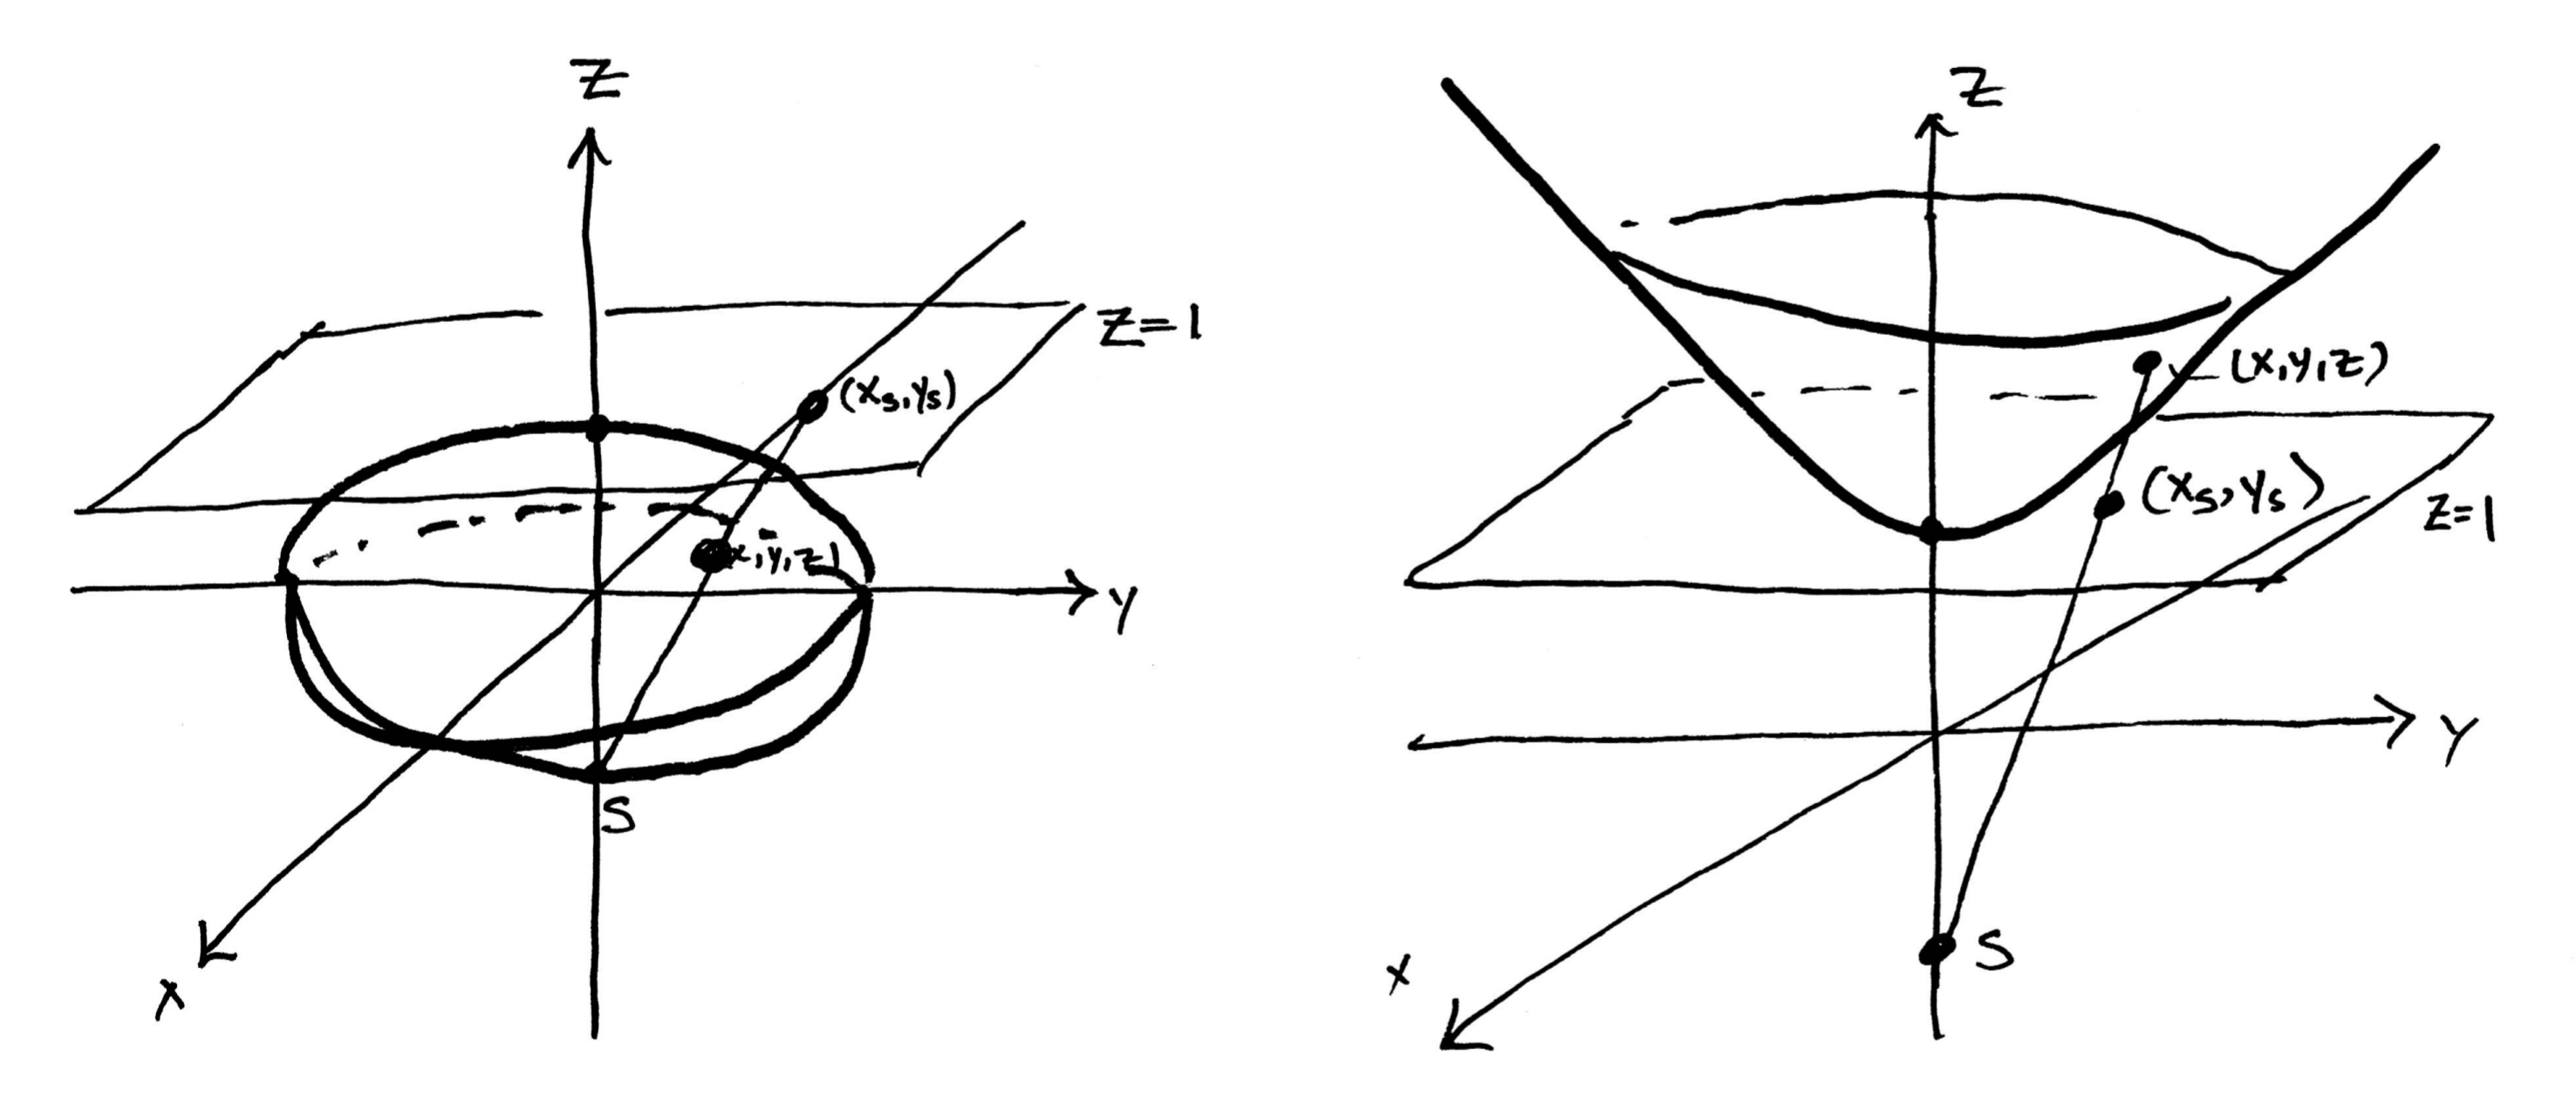
\includegraphics[width=5in]{stereoProj.png}
\end{image}
Let's look at this from a different vantage point, say with our eye
along the edge of the plane $z=1$:
\begin{image}
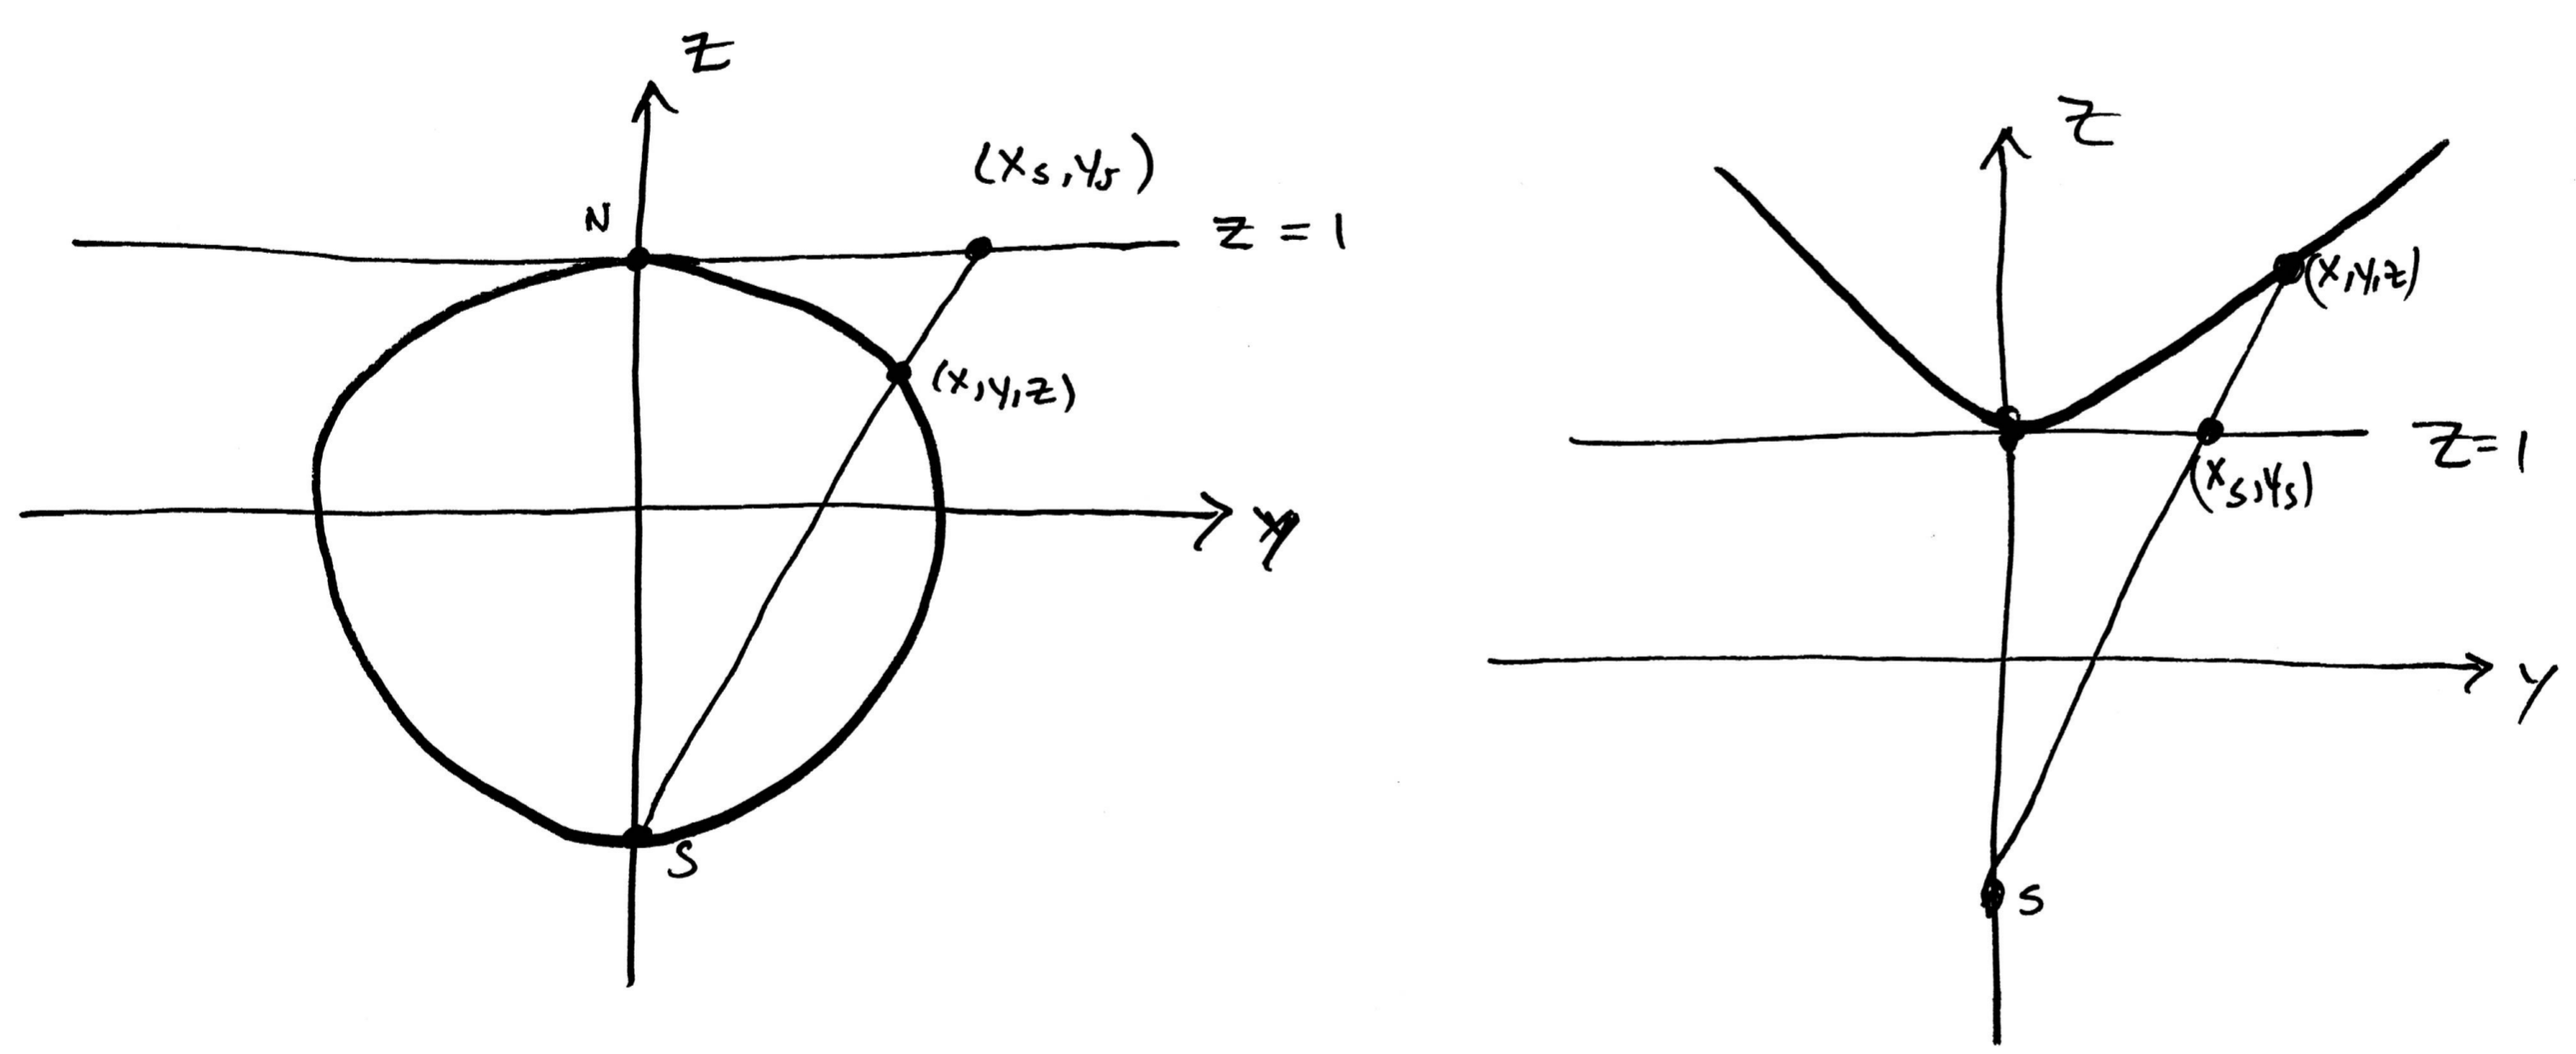
\includegraphics[width=5in]{stereoCross.png}
\end{image}

\begin{problem}
  If $K=1$ where does the `equator' map to? What about the `Northern hemisphere?' How about the `Southern hemisphere?'
  \begin{freeResponse}
    The `equator' maps to the circle of radius $2$ centered at the
    origin in the $(x_s,y_s)$ plane.  The `Northern hemisphere' maps
    inside this circle, and the `Southern hemisphere' maps outside the
    circle.
  \end{freeResponse}
\end{problem}

\begin{problem}
  Use similar triangles to explain why for any given $(x,y,z)$, there
  is a number $\rho$ such that
  \[
  \rho\cdot(x_s,y_s,2) = (x,y,z+1).
  \]
  \begin{freeResponse}
    Let $A = (x,y,z)$, $B= (x,y,-1)$, $A_s = (x_s,y_s,1)$ and
    $B_s=(x_s,y_s,-1)$. From the diagram above we see that
    \[
    \angle ASB = \angle A_s S B_s.
    \]
    Moreover, since $\triangle ASB$ and $\triangle A_s S B_s$ are
    right triangles, we now see that two of their angles have the same
    measure, and hence all three have the same measure. This means
    that these triangles are similar, and hence there they are
    dilations of one another. Hence there is a scale-factor $\rho$
    such that
    \[
    \rho\cdot(x_s,y_s,2) = (x,y,z+1).
    \]
  \end{freeResponse}
\end{problem}

\begin{problem}
  For the projection of the set $1=K\left(x^{2}+y^{2}\right)+z^{2}$
  onto the $z=1$ plane with center of projection $S$, write
  $(x_{s},y_{s})$ as a function of $(x,y,z)$.
  \begin{freeResponse}
    We know that
    \[
    \rho\cdot(x_{s},y_{s},2)=(x,y,z+1),
    \]
    hence $\rho=\frac{z+1}{2}$, and we may now write
    \begin{align*}
      x_{s} &=\frac{2x}{z+1},\\
      y_{s} &=\frac{2y}{z+1}.
    \end{align*}
  \end{freeResponse}
\end{problem}

\begin{problem}
  For the projection of the set $1=K\left(x^{2}+y^{2}\right)+z^{2}$
  onto the $z=1$ plane with center of projection $S$, write
  $(x,y,z)$ as a function of $(x_s,y_s)$.
  \begin{hint}
    Note that
      \[
      \rho\cdot(x_{s},y_{s},2)=(x,y,z+1) \qquad\text{and}\qquad z = 2\rho-1.
      \]
  \end{hint}
  \begin{hint}
    Hence if
    \[
    1 = K\left(x^2 + y^2\right) + z^2
    \]
    we may write
    \[
    1 = K\left((\rho\cdot x_s)^2 + (\rho\cdot y_s)^2\right) + (2\rho-1)^2
    \]
    and solve for $\rho$.
  \end{hint}
  \begin{freeResponse}
    This is slightly more complex than the previous problem; however,
    we will begin the same way. We know that
    \[
    \rho\cdot(x_{s},y_{s},2)=(x,y,z+1),
    \]
    hence $\rho=\frac{z+1}{2}$, and we may now write
    \begin{align*}
      x &= \rho \cdot x_s,\\
      y &= \rho \cdot y_s,\\
      z &= 2\rho-1.
    \end{align*}
    Now our task is to write $\rho$ in terms of $x_s$ and
    $y_s$. Using our assignments above, write
    \begin{align*}
      1 &= K\left(x^2 + y^2\right) + z^2\\
      1 &= K\left((\rho\cdot x_s)^2 + (\rho\cdot y_s)^2\right) + (2\rho-1)^2\\
      1 &= K\left((\rho\cdot x_s)^2 + (\rho\cdot y_s)^2\right) + 4\rho^2-4\rho + 1\\
    \end{align*}
    and so
    \begin{align*}
      0 &= K\left(\rho^2\cdot x_s^2 + \rho^2\cdot y_s^2\right) + 4\rho^2-4\rho\\
      0 &= \rho^2\cdot K\left(x_s^2 + y_s^2\right) + 4\rho^2-4\rho
    \end{align*}
    and since $\rho \ne 0$, we may write
    \begin{align*}
      \rho\cdot K\left(x_s^2 + y_s^2\right) + 4\rho-4 &=0 \\
      \rho\left(K\left(x_s^2 + y_s^2\right) + 4\right) &=4\\
      \rho &= \frac{4}{K\left(x_s^2 + y_s^2\right) + 4}.
    \end{align*}
    Hence
    \begin{align*}
      x &= \frac{4x_s}{K\left(x_s^2 + y_s^2\right) + 4},\\
      y &= \frac{4y_s}{K\left(x_s^2 + y_s^2\right) + 4},\\
      z &= \frac{4-K\left(x_s^2 + y_s^2\right)}{4+K\left(x_s^2 + y_s^2\right)}.\\
    \end{align*}
  \end{freeResponse}
\end{problem}


\section{Stereographic projection dot product}

Once more, we want to be able to find a dot product that will allow us
to compute lengths in stereographic projection coordinates that will agree
with the $K$-dot product, and hence the euclidean dot product.

\begin{problem}
Suppose we have a curve $X$ in $K$-warped space that is a function of
a curve $X_s$ in the plane $z=1$ space. So
\[
X_s(t) = \left( x_s(t),y_s(t)\right)
\]
and
\[
X(t) = 
\begin{cases}
  x(x_s(t),y_s(t)),\\
  y(x_s(t),y_s(t)),\\
  z(x_s(t),y_s(t)).
\end{cases}
\]
Use the chain rule to compute
\[
\dd[x]{t}, \qquad \dd[y]{t}, \qquad \dd[z]{t},
\]
in terms of $\dd[x_s]{t}$, $\dd[y_s]{t}$, $\pp[x]{x_s}$,
$\pp[y]{x_s}$, $\pp[z]{x_s}$, $\pp[x]{y_s}$, $\pp[y]{y_s}$,
and $\pp[z]{y_s}$.
  \begin{hint}
  Simply write down the answer from a previous problem with some minor
  changes.
  \end{hint}
  \begin{freeResponse}
  Write
  \begin{align*}
    \dd[x]{t} &= \begin{bmatrix}\pp[x]{x_s} & \pp[x]{y_s}\end{bmatrix}\cdot\begin{bmatrix}\dd[x_s]{t} & \dd[y_s]{t}\end{bmatrix}^\transpose = \pp[x]{x_s}\cdot\dd[x_s]{t}+\pp[x]{y_s}\cdot\dd[y_s]{t},   \\
    \dd[y]{t} &= \begin{bmatrix}\pp[y]{x_s} & \pp[y]{y_s}\end{bmatrix}\cdot\begin{bmatrix}\dd[x_s]{t} & \dd[y_s]{t}\end{bmatrix}^\transpose = \pp[y]{x_s}\cdot\dd[x_s]{t}+\pp[y]{y_s}\cdot\dd[y_s]{t},   \\
    \dd[z]{t} &= \begin{bmatrix}\pp[z]{x_s} & \pp[z]{y_s}\end{bmatrix}\cdot\begin{bmatrix}\dd[x_s]{t} & \dd[y_s]{t}\end{bmatrix}^\transpose = \pp[z]{x_s}\cdot\dd[x_s]{t}+\pp[z]{y_s}\cdot\dd[y_s]{t}.  
  \end{align*}
\end{freeResponse}
\end{problem}


\begin{problem}
  With the same setting as in the previous problem, rewrite the result
  of your computation in matrix notation to find $D_s$
  such that
\[
\begin{bmatrix}
\dd[x]{t} & \dd[y]{t} & \dd[z]{t}
\end{bmatrix}
=
\begin{bmatrix}
\frac{dx_s}{dt} & \frac{dy_s}{dt}
\end{bmatrix}\cdot D_s
\]
in terms of $\pp[x]{x_s}$, $\pp[y]{x_s}$, $\pp[z]{x_s}$,
$\pp[x]{y_s}$, $\pp[y]{y_s}$, and $\pp[z]{y_s}$.
\begin{hint}
  Simply write down the answer from a previous problem with some minor
  changes.
\end{hint}
\begin{freeResponse}
  \[
  D_s =
  \begin{bmatrix}
    \pp[x]{x_s} & \pp[y]{x_s} & \pp[z]{x_s} \\
    \pp[x]{y_s}   & \pp[y]{y_s}   & \pp[z]{y_s}
  \end{bmatrix}.
  \]
\end{freeResponse}
\end{problem}

\begin{problem}
  Now find $P_s$ in terms of $K$, $\pp[x]{x_s}$, $\pp[y]{x_s}$,
  $\pp[z]{x_s}$, $\pp[x]{y_s}$, $\pp[y]{y_s}$, and $\pp[z]{y_s}$ such
  that
  \[
  \left(\dd[x]{t}, \dd[y]{t}, \dd[z]{t}\right)\bullet_K
  \left(\dd[x]{t}, \dd[y]{t}, \dd[z]{t}\right)
  =
  \begin{bmatrix}
    \dd[x_s]{t} &  \dd[y_s]{t}
  \end{bmatrix}
  \cdot P_s
  \cdot
  \begin{bmatrix}
    \dd[x_s]{t} \\  \dd[y_s]{t}
  \end{bmatrix}.
  \]
  \begin{hint}
  Simply write down the answer from a previous problem with some minor
  changes.
  \end{hint}
  \begin{freeResponse}
    For completeness sake, we will include a complete solution.
    Working from the $K$-dot product, we need that
    \begin{align*}
    \left(\dd[x]{t}, \dd[y]{t}, \dd[z]{t}\right)\bullet_K
    \left(\dd[x]{t}, \dd[y]{t}, \dd[z]{t}\right)
    &=
    \begin{bmatrix}
      \dd[x]{t} & \dd[y]{t} & \dd[z]{t}
    \end{bmatrix}
    \begin{bmatrix}
      1 & 0 & 0\\
      0 & 1 & 0\\
      0 & 0 & K^{-1}
    \end{bmatrix}
    \begin{bmatrix}
      \dd[x]{t} \\ \dd[y]{t} \\ \dd[z]{t}
    \end{bmatrix}\\
    &=
    \begin{bmatrix}
      \frac{dx_s}{dt} & \frac{dy_s}{dt}
    \end{bmatrix}\cdot D_{s}\cdot
    \begin{bmatrix}
      1 & 0 & 0\\
      0 & 1 & 0\\
    0 & 0 & K^{-1}
    \end{bmatrix}
    \cdot
    \left(
    \begin{bmatrix}
      \frac{dx_s}{dt} & \frac{dy_s}{dt}
    \end{bmatrix}\cdot D_{s}
    \right)^\transpose\\
    &=
    \begin{bmatrix}
      \frac{dx_s}{dt} & \frac{dy_s}{dt}
    \end{bmatrix}\cdot D_{s}\cdot
    \begin{bmatrix}
      1 & 0 & 0\\
      0 & 1 & 0\\
    0 & 0 & K^{-1}
    \end{bmatrix}
    \cdot
    D_{s}^\transpose
    \cdot \begin{bmatrix}
      \frac{dx_s}{dt} \\ \frac{dy_s}{dt}
    \end{bmatrix}.
  \end{align*}
    Hence
    \begin{align*}
      P_s &=
      \begin{bmatrix}
        \pp[x]{x_s} & \pp[y]{x_s} & \pp[z]{x_s} \\
        \pp[x]{y_s} & \pp[y]{y_s} & \pp[z]{y_s}
      \end{bmatrix}
      \begin{bmatrix}
        1 & 0 & 0\\
        0 & 1 & 0\\
        0 & 0 & K^{-1}
      \end{bmatrix}
      \begin{bmatrix}
        \pp[x]{x_s} & \pp[x]{y_s}\\ 
        \pp[y]{x_s} & \pp[y]{y_s}\\
        \pp[z]{x_s} & \pp[z]{y_s}
      \end{bmatrix}\\
      &=
      \begin{bmatrix}
        \left(\pp[x]{x_s}\right)^2 + \left(\pp[y]{x_s}\right)^2 + \left(\pp[z]{x_s}\right)^2K^{-1} & \pp[x]{x_s}\pp[x]{y_s} + \pp[y]{x_s}\pp[y]{y_s} + \pp[z]{x_s}\pp[z]{y_s} K^{-1}\\
        \pp[x]{x_s}\pp[x]{y_s} + \pp[y]{x_s}\pp[y]{y_s} + \pp[z]{x_s}\pp[z]{y_s} K^{-1}       & \left(\pp[x]{y_s}\right)^2 + \left(\pp[y]{y_s}\right)^2 + \left(\pp[z]{y_s}\right)^2K^{-1}
      \end{bmatrix}.
    \end{align*}
  \end{freeResponse}
\end{problem}


Before we actually compute $P_s$, it will help to compute the partial
derivatives.


\begin{problem}
  Set
  \begin{align*}
    x(x_s,y_s) &=\rho\cdot x_s,\\
    y(x_s,y_s) &=\rho\cdot y_s,\\
    z(x_s,y_s) &=2\rho-1,
  \end{align*}
  and show that
  \[
  \begin{split}
    \pp[x]{x_s} &=\rho-\left(\frac{K}{2}\right)\rho^2x_s^2,\\
    \pp[y]{x_s} &=-\left(\frac{K}{2}\right)\rho^2x_sy_s,\\
    \pp[z]{x_s} &=-K\rho^2x_s,
  \end{split}
  \qquad
  \begin{split}
    \pp[x]{y_s} &= -\left(\frac{K}{2}\right)\rho^2x_sy_s,\\
    \pp[y]{y_s} &=\rho-\left(\frac{K}{2}\right)\rho^2y_s^2,\\
    \pp[z]{y_s} &= -K\rho^2y_s.
  \end{split}
  \]
  \begin{hint}
  Work in the following way:
  \begin{enumerate}
  \item Recall $x = \rho\cdot x_s$.
  \item Note that $\pp[x]{x_s} = \rho + x_s \cdot \pp[\rho]{x_s}$.
  \item Express the partial derivative in terms of $\rho$, $K$, $x_s$,
      and $y_s$.
  \end{enumerate}
  \end{hint}
  \begin{freeResponse}
    Write
    \begin{align*}
      \pp[x]{x_s} &= \rho + x_s\cdot \pp[\rho]{x_s}\\
      &= \rho + x_s\cdot \pp{x_s}\left(\frac{4}{K\left(x_s^2 + y_s^2\right) + 4}\right)\\
      &= \rho - x_s\cdot \left(\frac{4}{\left(K\left(x_s^2 + y_s^2\right) + 4\right)^{2}}\right)\cdot2Kx_s \\
      &=\rho-\left(\frac{K}{2}\right)\rho^2x_s^2.
    \end{align*}
    Similarly,
      \begin{align*}
      \pp[y]{x_s} &= y_s\cdot \pp[\rho]{x_s}\\
      &= y_s\cdot \pp{x_s}\left(\frac{4}{K\left(x_s^2 + y_s^2\right) + 4}\right)\\
      &= - y_s\cdot \left(\frac{4}{\left(K\left(x_s^2 + y_s^2\right) + 4\right)^{2}}\right)\cdot2Kx_s \\
      &= -\left(\frac{K}{2}\right)\rho^2x_sy_s.
      \end{align*}
      Finally,
      \begin{align*}
      \pp[z]{x_s} &= 2\cdot\pp[\rho]{x_s}\\
      &= 2\cdot\cdot \pp{x_s}\left(\frac{4}{K\left(x_s^2 + y_s^2\right) + 4}\right)\\
      &= - 2\cdot \left(\frac{4}{\left(K\left(x_s^2 + y_s^2\right) + 4\right)^{2}}\right)\cdot2Kx_s \\
      &= -\frac{K}\rho^2x_s.
      \end{align*}
      Now with entirely similar computations, we see
      \begin{align*}
        \pp[x]{y_s} &= -\left(\frac{K}{2}\right)\rho^2x_sy_s,\\
        \pp[y]{y_s} &=\rho-\left(\frac{K}{2}\right)\rho^2y_s^2,\\
        \pp[z]{y_s} &= -K\rho^2y_s.       
      \end{align*}
  \end{freeResponse}
\end{problem}


\begin{problem}
With the same setting as above, show that $P_s$ is
  \[
  P_s =
  \begin{bmatrix}
    \rho^2 & 0\\
    0 & \rho^2
  \end{bmatrix}.
  \]
  \begin{hint}
  When simplifying, combine the terms with the highest degree of $\rho$
  and note that
  \[
  \rho^{-1} = \frac{K\left(x_s^2 + y_s^2\right)+4}{4}.
  \]
\end{hint}
\begin{freeResponse}
  Write $\left(\pp[x]{x_s}\right)^2 + \left(\pp[y]{x_s}\right)^2 +\left(\pp[z]{x_s}\right)^2K^{-1}$
  \begin{align*}
    &=\left(\rho-\left(\frac{K}{2}\right)\rho^2x_s^2\right)^2 + \left(-\left(\frac{K}{2}\right)\rho^2x_sy_s\right)^2 +\left(-K\rho^2x_s\right)^2K^{-1}\\
    &=\rho^2 -K\rho^3x_s^2 + \left(\frac{K^2}{4}\right)\rho^4x_s^4 + \left(\frac{K^2}{4}\right)\rho^4x_s^2y_s^2 + K\rho^4x_s^2\\
    &=\rho^2 -K\rho^3x_s^2 + K\rho^4x_s\left(\left(\frac{K}{4}\right)x_s^4 + \left(\frac{K}{4}\right)y_s^2 + 1\right)\\
    &=\rho^2 -K\rho^3x_s^2 + K\rho^4x_s\left(\frac{K\left(x_s^2+y_s^2\right)+4}{4}\right)\\
    &=\rho^2 -K\rho^3x_s^2 + K\rho^4x_s\rho^{-1}\\
    &=\rho^2.
  \end{align*}
  That $\pp[x]{x_s}\pp[x]{y_s} + \pp[y]{x_s}\pp[y]{y_s} + \pp[z]{x_s}\pp[z]{y_s} K^{-1}$
  \begin{align*}
    &=\left(\rho-\left(\frac{K}{2}\right)\rho^2x_s^2\right)\left(-\left(\frac{K}{2}\right)\rho^2x_sy_s\right)
    + \left(-\left(\frac{K}{2}\right)\rho^2x_sy_s\right)\left(\rho-\left(\frac{K}{2}\right)\rho^2y_s^2\right)
    + \left(-K\rho^2x_s\right)\left(-K\rho^2y_s\right) K^{-1}\\
    &=
    -\left(\frac{K}{2}\right)\rho^3x_sy_s+\left(\frac{K^2}{4}\right)\rho^4x_s^3y_s
    -\left(\frac{K}{2}\right)\rho^3x_sy_s+\left(\frac{K^2}{4}\right)\rho^4x_sy_s^3
    + K\rho^4 x_sy_s\\
    &= -K\rho^3x_sy_s + K\rho^4x_sy_s\left(\frac{K\left(x_s^2+y_s^2\right)+4}{4}\right)\\
    &= -K\rho^3x_sy_s + K\rho^4x_sy_s\rho^{-1}\\
    &= -K\rho^3x_sy_s + K\rho^3x_sy_s\\
    &=0.
  \end{align*}
  With entirely analogous computations, we see that 
    \[
    P_s =
    \begin{bmatrix}
      \rho^2 & 0\\
      0 & \rho^2
    \end{bmatrix}.
    \]
\end{freeResponse}
\end{problem}

\begin{definition}
  Let $V_s$ and $W_s$ be a vectors in $(x_s,y_s)$-coordinates
  originating at the same $(x_s,y_s)$-coordinate. Define
  \[
  V_s \bullet_s W_s = V_s \cdot P_s \cdot W_s^\transpose
  \]
  where
  \[
  P_s =
  \begin{bmatrix}
    \rho^2 & 0\\
    0 & \rho^2
  \end{bmatrix}
  \]
  is determined by the coordinate that the vectors originate from.
\end{definition}








\section{Again, when the finite is infinite and the infinite is finite}

Just like central projection, stereographic projection allows us to
think about both ``finite'' areas and ``infinite'' areas in new ways.

\paragraph{When $K$ is positive, the finite is infinite}

When $K>0$, we are working with a sphere. As we know, a sphere has
finite surface area.



\begin{problem}
  Where does the Northeren hemisphere of the $R$-sphere map to under stereographic projection?
  \begin{hint}
    A picture is worth a thousand words!
  \end{hint}
  \begin{freeResponse}
  \end{freeResponse}
\end{problem}


\begin{problem}
  Where does the Southeren hemisphere of the $R$-sphere map to under stereographic projection?
  \begin{hint}
    A picture is worth a thousand words!
  \end{hint}
  \begin{freeResponse}
  \end{freeResponse}
\end{problem}


\begin{problem}
  As a point approaches the South Pole of the $R$-sphere where does it
  move to under stereographic projection?
  \begin{hint}
    Simply transform the relevant coordinate.
  \end{hint}
  \begin{freeResponse}
  \end{freeResponse}
\end{problem}



\begin{problem}
  Explain why one might say that stereographic projection makes the
  ``finite'' seem ``infinite.''
    \begin{freeResponse}
    \end{freeResponse}
\end{problem}




\paragraph{When $K$ is negative, the infinite is finite}


Notice that, if $K<0$, the equation of $K$-geometry becomes
\[
z^{2}-|K|\left(x^{2}+y^{2}\right)  =1.
\]
This describes a $K$-geometry forms a $2$-sheeted hyperboloid with the
$z$-axis as major axis. We will only consider the sheet on which $z$
is positive as forming the $K$-geometry.  Of critical importance, note

\begin{center}
  \textbf{this hyperboloid has infinite surface area.}
\end{center}

The hyperboloid above is obtained by rotating the hyperbola
\[
z^{2}-\left\vert K\right\vert x^{2}= 1
\]
in the $(x,z)$-plane around the $z$-axis.



\begin{problem}
  Assume we have a point in $K$-geometry that is shooting off to
  infinity. What is the maximum distance the image of this point can
  be from the origin in stereographic projection?
  \begin{hint}
    First rewrite $z^{2}-|K|x^{2} =1$ as
    \[
    z = \sqrt{1+|K|x^2}
    \]
    and explain why this is acceptable.
  \end{hint}
  \begin{hint}
    Explain why computing this limit
    \[
    \lim_{x\to \infty} \frac{\sqrt{1+|K|x^2}}{x}
    \]
    helps us in this context.
  \end{hint}
  \begin{freeResponse}
    Since we are only considering the upper hyperboloid, we need only
    look at the upper hyperbola. Hence we may look at
     \[
    z = \sqrt{1+|K|x^2}.
    \]
    To compute the maximum distance the image of a point can be from
    the origin, look at 
    \[
    \lim_{x\to \infty} \frac{\sqrt{1+|K|x^2}}{x}
    \]
    as this computes the ``end-behavior'' of the ``slope'' of the
    curve. Write
    \begin{align*}
      \lim_{x\to \infty} \frac{\sqrt{1+|K|x^2}}{x} &= \lim_{x\to \infty} \frac{\sqrt{1+|K|x^2}}{x}\cdot \frac{1/x}{1/x}\\
      &= \lim_{x\to \infty} \sqrt{1/x^2+|K|}\\
      &= \sqrt{|K|}.
    \end{align*}
    Hence one projection is given by $z = x\sqrt{|K|}-1$.
  \end{freeResponse}
\end{problem}


Rotating the line found above gives the ``asymptotic cone.'' The
stereographic projection coordinates $(x_{s},y_{s})$ of $K$-geometry
when $K<0$ only correspond to points in $K$-geometry when
$(x_{s},y_{s},1)$ lies \textit{inside} the asymptotic cone.

\begin{problem}
  When $K<0$, find the radius of the disk in the plane $z=1$ whose
  perimeter is determined by the asymptotic cone. 
  \begin{hint}
    Work with the asymptote(s) you found above.
  \end{hint}
  \begin{freeResponse}
    We must find where $z = x\sqrt{|K|}-1$ intersects the line $z=1$. To do this, simply solve
    \[
    1 = x\sqrt{|K|}-1
    \]
    for $x$, and so the radius is $2/\sqrt{|K|}$.
  \end{freeResponse}
\end{problem}

\begin{problem}
  Explain why one might say that stereographic projection makes the
  ``infinite'' seem ``finite.''
    \begin{freeResponse}
    \end{freeResponse}
\end{problem}

The $(x_{s},y_{s})$-coordinates are called \dfn{Poincar\'e
  coordinates} for hyperbolic geometry and the disk of radius
$2/\sqrt{|K|}$ called the \dfn{Poincar\'e model} for hyperbolic
geometry in honor of the famous French geometer, Henri Poincar\'e.









\begin{problem}
Summarize the results from this section. In particular, indicate which
results follow from the others.
\begin{freeResponse}
\end{freeResponse}
\end{problem}


\end{document}

\end{masterdocument}
